
\documentclass[a4paper,twoside,12pt]{book}
\usepackage[utf8]{inputenc}                                      
\usepackage[T1]{fontenc}  
\usepackage{amsmath,amsfonts,amssymb,amsthm}
\usepackage[british,polish]{babel} 
\usepackage{indentfirst}
\usepackage{lmodern}
\usepackage{graphicx} 
\usepackage{hyperref}
\usepackage{booktabs}
%\usepackage{tikz}
%\usepackage{pgfplots}
\usepackage{mathtools}
\usepackage{geometry}
\usepackage{float}
\usepackage{afterpage}
\usepackage{placeins}
\usepackage{url}
\usepackage[page]{appendix} % toc,
\renewcommand{\appendixtocname}{Dodatki}
\renewcommand{\appendixpagename}{Dodatki}
\renewcommand{\appendixname}{Dodatek}

\usepackage{setspace}
\onehalfspacing

\usepackage{caption}
\DeclareCaptionLabelSeparator{dotLabel}{.\space}
\captionsetup{labelsep=dotLabel}
\captionsetup[lstlisting]{justification=centering}

\frenchspacing

\usepackage{listings}
%\lstset{
%	language={},
%	basicstyle=\ttfamily,
%	keywordstyle=\lst@ifdisplaystyle\color{blue}\fi,
%	commentstyle=\color{gray}
%}

%%%%%%%%%%%%%%%%%%%%%%%%%%%
% listingi 
\usepackage{listings}
\lstset{%
aboveskip=20pt,
belowskip=0pt,
language=[Sharp]C,%
showspaces=false,%
commentstyle=\textit,%
identifierstyle=\textsf,%
keywordstyle=\sffamily\bfseries, %\texttt, %
captionpos=b,%
tabsize=2,%
frame=lines,%
numbers=left,%
numberstyle=\tiny,%
numbersep=5pt,%
breaklines=true,%
%morekeywords={},%
escapeinside={@*}{*@},%
%texcl=true, % wylacza tryb verbatim w komentarzach jednolinijkowych
}

\renewcommand{\lstlistingname}{Kod}
\renewcommand{\lstlistlistingname}{Spis źródeł}
%%%%%%%%%%%%%%%%%%%%%%%%%%%%%%%%%%%%


%%%%%%%%%

%%%% TODO LIST GENERATOR %%%%%%%%%

%\usepackage{tikz}
%\usepackage{manfnt}   % dangerous sign 
\usepackage{color}
\definecolor{brickred}      {cmyk}{0   , 0.89, 0.94, 0.28}

\makeatletter \newcommand \kslistofremarks{\section*{Uwagi} \@starttoc{rks}}
  \newcommand\l@uwagas[2]
    {\par\noindent \textbf{#2:} %\parbox{10cm}
{#1}\par} \makeatother


\newcommand{\ksremark}[1]{%
{%\marginpar{\textdbend}
{\color{brickred}{[#1]}}}%
\addcontentsline{rks}{uwagas}{\protect{#1}}%
}

\newcommand{\comma}{\ksremark{przecinek}}
\newcommand{\nocomma}{\ksremark{bez przecinka}}
\newcommand{\styl}{\ksremark{styl}}
\newcommand{\ortografia}{\ksremark{ortografia}}
\newcommand{\fleksja}{\ksremark{fleksja}}
\newcommand{\pauza}{\ksremark{pauza `--', nie dywiz `-'}}
\newcommand{\kolokwializm}{\ksremark{kolokwializm}}

%%%%%%%%%%%%%% END OF TODO LIST GENERATOR %%%%%%%%%%%

%%%%%%%%%%%% ZYWA PAGINA %%%%%%%%%%%%%%%
% brak kapitalizacji zywej paginy
\usepackage{fancyhdr}
\pagestyle{fancy}
\fancyhf{}
\fancyhead[LO]{\nouppercase{\it\rightmark}}
\fancyhead[RE]{\nouppercase{\it\leftmark}}
\fancyhead[LE,RO]{\it\thepage}


\fancypagestyle{tylkoNumeryStron}{%
   \fancyhf{} 
   \fancyhead[LE,RO]{\it\thepage}
}

\fancypagestyle{NumeryStronNazwyRozdzialow}{%
   \fancyhf{} 
   \fancyhead[LO]{\nouppercase{\it\rightmark}}
   \fancyhead[RE]{\nouppercase{\it\leftmark}}
   \fancyhead[LE,RO]{\it\thepage}
}


%%%%%%%%%%%%% OBCE WTRETY  
\newcommand{\obcy}[1]{\emph{#1}}
\newcommand{\ang}[1]{{\selectlanguage{british}\obcy{#1}}}
%%%%%%%%%%%%%%%%%%%%%%%%%%%%%

% polskie oznaczenia funkcji matematycznych
\renewcommand{\tan}{\operatorname {tg}}
\renewcommand{\log}{\operatorname {lg}}

% jeszcze jakies drobiazgi

\newcounter{stronyPozaNumeracja}

\newcommand{\hcancel}[1]{%
    \tikz[baseline=(tocancel.base)]{
        \node[inner sep=0pt,outer sep=0pt] (tocancel) {#1};
        \draw[red] (tocancel.south west) -- (tocancel.north east);
    }%
}%

\newcommand{\miesiac}{%
  \ifcase\the\month
  \or styczeń% 1
  \or luty% 2
  \or marzec% 3
  \or kwiecień% 4
  \or maj% 5
  \or czerwiec% 6
  \or lipiec% 7
  \or sierpień% 8
  \or wrzesień% 9
  \or październik% 10
  \or listopad% 11
  \or grudzień% 12
  \fi}


%%%%%%%%%%%%%%%%%%%%%%%%%%%%%%%%%%%%%%%%%%%%%%
% Helvetica font macros for the title page:
\newcommand{\headerfont}{\fontfamily{phv}\fontsize{18}{18}\bfseries\scshape\selectfont}
\newcommand{\titlefont}{\fontfamily{phv}\fontsize{18}{18}\selectfont}
\newcommand{\otherfont}{\fontfamily{phv}\fontsize{14}{14}\selectfont}

%%%%%%%%%%%%%%%%%%%%%%%%%%%%%%%%%%%%%%%%%%%%%%
%%%%%%%%%%%%%%%%%%%%%%%%%%%%%%%%%%%%%%%%%%%%%%
%%%%%%%%%%%%%%%%%%%%%%%%%%%%%%%%%%%%%%%%%%%%%%
%%%%%%%%%%%%%%%%%%%%%%%%%%%%%%%%%%%%%%%%%%%%%%
%%%%%%%%%%%%%%%%%%%%%%%%%%%%%%%%%%%%%%%%%%%%%%
%%%%%%%%%%%%%%%%%%%%%%%%%%%%%%%%%%%%%%%%%%%%%%
%%%%%%%%%%%%%%%%%%%%%%%%%%%%%%%%%%%%%%%%%%%%%%


\newcommand{\autor}{Seweryn Gładysz}
\newcommand{\promotor}{dr inż. Ewa Płuciennik}
\newcommand{\tytul}{System zarządzania siecią siłowni oparty o bazę dokumentową}
\newcommand{\polsl}{Politechnika Śląska}
\newcommand{\wydzial}{Wydział Automatyki, Elektroniki i Informatyki}
\newcommand{\kierunek}{Kierunek: Informatyka}


\begin{document}
%\kslistofremarks 
	
%%%%%%%%%%%%%%%%%%  STRONA TYTULOWA %%%%%%%%%%%%%%%%%%%
\pagestyle{empty}
{
	\newgeometry{top=2.5cm,%
	             bottom=2.5cm,%
	             left=3cm,
	             right=2.5cm}
	\sffamily
	\rule{0cm}{0cm}
	
	\begin{center}
	
\includegraphics[width=29mm]{logo_pl.jpg}
	\end{center} 
	\vspace{1cm}
	\begin{center}
	\headerfont \polsl
	\end{center}
	\begin{center}
	\headerfont \wydzial
	\end{center}
	\begin{center}
	\headerfont \kierunek
	\end{center}
	\vfill
	\begin{center}
	\titlefont Praca dyplomowa inżynierska
	\end{center}
	\vfill
	
	\begin{center}
	\otherfont \tytul\par
	\end{center}
	
	\vfill
	
	\vfill
	 
	\noindent\vbox
	{
		\hbox{\otherfont autor: \autor}
		\vspace{12pt}
		\hbox{\otherfont kierujący pracą: \promotor}
		% \vspace{12pt}  % zakomentuj, jezeli nie ma konsultanta
		% \hbox{\otherfont konsultant: \konsultant} % zakomentuj, jezeli nie ma konsultanta
	}
	\vfill 
 
   \begin{center}
   \otherfont Gliwice,  \miesiac\ \the\year
   \end{center}	
	\restoregeometry
}
  

\cleardoublepage
 

\rmfamily
\normalfont


%%%%%%%%%%%%%%%%%% SPIS TRESCI %%%%%%%%%%%%%%%%%%%%%%
\pagenumbering{Roman}
\pagestyle{tylkoNumeryStron}
\tableofcontents

%%%%%%%%%%%%%%%%%%%%%%%%%%%%%%%%%%%%%%%%%%%%%%%%%%%%%
\setcounter{stronyPozaNumeracja}{\value{page}}
\mainmatter
\pagestyle{empty}

\chapter*{Streszczenie}

Czas pandemii koronawirusa stawia przed przedsiębiorcami nowe wyzwania, a cyfryzacja pozwala na automatyzację wielu czynności. Właściciele sieci siłowni są zmuszeni do ciągłego dostosowywania zasad działania siłowni do wymogów związanych z obostrzeniami sanitarnymi. Dzięki rozwojowi aplikacji internetowych istnieje możliwość zarządzania biznesem zarówno z poziomu komputera osobistego jak i smartfona.

W pracy przedstawiono projekt aplikacji internetowej, która pozwala na zarządzanie siecią obiektów siłowni. Szczególny nacisk położono na możliwość definiowania zasad działania poszczególnych obiektów w kontekście obowiązujących restrykcji sanitarnych. System korzysta z dokumentowej bazy danych w celu skorzystania z zalet technologii \textit{NoSQL}. Warstwa prezentacji wykorzystuje możliwości współczesnych przeglądarek internetowych.

W ramach pracy omówiono ideę stojącą za stworzeniem systemu oraz sposób jego projektowania. Opisane zostały metodyki pracy nad projektem, wykorzystane technologie oraz wybrane wzorce projektowe, które zostały użyte przy pracy nad aplikacją.

{\bf Slowa kluczowe: NoSQL, MongoDB, sieć siłowni}

\addcontentsline{toc}{chapter}{Streszczenie}

\cleardoublepage

\pagestyle{NumeryStronNazwyRozdzialow}

%%%%%%%%%%%%%% wlasciwa tresc pracy %%%%%%%%%%%%%%%%%

\chapter{Wstęp}

Głównym celem tego projektu jest stworzenie systemu informatycznego pozwalającego na prowadzenie sieci siłowni z wykorzystaniem dokumentowej bazy danych. Podstawowym założeniem projektu jest przygotowanie systemu w taki sposób, aby właściciele mogli dostosowywać zasady działania obiektów sportowych do aktualnie obowiązujących restrykcji sanitarnych. Prowadzenie obiektu siłowni jest utrudnione w czasie pandemii ze względu na częste zmiany w przepisach związanych z ograniczeniami pandemicznymi. Wymienione wcześniej problemy były głównym powodem powstania tego projektu.

Wykorzystanie dokumentowej bazy danych jest związane z zaletami baz \textit{NoSQL}. Niektóre cechy wcześniej wymienionych baz nie są dostępne dla relacyjnych baz danych. Jedną z takich cech jest duża podatność na zmiany w strukturze względem relacyjnych baz oraz przystosowanie do skalowania wszerz \cite{bib:noSqlVsSql}.

Pracę podzielono na rozdziały, gdzie pierwszy został poświęcony analizie tematu. Analiza zawiera informacje o idei powstania systemu oraz wyzwaniach z~którymi projekt będzie musiał się mierzyć. Kolejny rozdział został poświęcony wymaganiom i narzędziom. Wymagania w rozdziale \ref{chap:Wymagania} zostały podzielone na funkcjonalne i niefunkcjonalne, a w kolejnych podrozdziałach opisano narzędzia, które wykorzystano do ich realizacji. Rozdział \ref{chap:external} opisuje wymagania sprzętowe, kategorie użytkowników oraz przykłady działania aplikacji. Poza tym zawiera wyczerpującą instrukcję instalacji i uruchamiania systemu. W rozdziale \ref{chap:internal} skupiono się na opisie architektury i przyjętej organizacji bazy danych. W kolejnych podrozdziałach przedstawiono przegląd najważniejszych klas i wzorców projektowych. Rozdział \ref{chap:validation} poświęcono testom jakim został poddany system. W ramach rozdziału opisano sposoby i organizacje testów z podziałem na testy jednostkowe i manualne. Ostatni rozdział \ref{chap:summary} przedstawia wnioski i obserwacje do jakich doszło w trakcie prac. Rozdział kończy się przedstawieniem propozycji usprawnienia systemu w przypadku kontynuowania pracy nad nim.

\chapter{Analiza tematu}
Na rynku siłowni widać coraz większą konkurencję, a właściciele szukają sposobów jak zachęcić nowych klientów do uczęszczania na ich siłownie. Wiele z sieci pozwala na całodobowe korzystanie z ich obiektów, aby sprostać wymaganiom jak największej grupy klientów. Stawia to nowe wyzwania w organizacji pracy i sposobie działania obiektów. Dużym usprawnieniem byłaby możliwość zrezygnowania z~recepcji na rzecz bramek wejściowych i wyjściowych, które kontrolowałby ważność karnetu oraz pilnowałby, aby w tej samej chwili na siłowni nie znajdowała się zbyt duża liczba osób.

Innym problemem jest coraz większa liczba sieci siłowni, która w swojej ofercie zawiera możliwość udziału w wydarzeniach grupowych, które pozwalają na uczestnictwo w grupowej sesji, gdzie pracownik siłowni nadzoruje czy uczestnicy wykonują ćwiczenia w sposób bezpieczny dla ich zdrowia. Pozwolenie na zgłoszenie chęci udziału w takim wydarzeniu poprzez aplikację internetową może zwiększyć atrakcyjność oferty danej sieci siłowni w obliczu rosnącej konkurencji na rynku sieci siłowni.

Sieć siłowni zderza się z problemami, które nie są znane pojedynczym obiektom. Zarządzanie wyposażeniem może być utrudnione ze względu na liczbę posiadanych urządzeń i liczbę obiektów siłowni należących do sieci. System powinien gromadzić informacje na temat posiadanego sprzętu, aby skrócić czas, jaki jest potrzebny do przeprowadzenia inwentaryzacji posiadanych akcesoriów i sprzętów do ćwiczeń.

Innym wyzwaniem stawianym przed właścicielami siłowni jest stworzenie oferty treningów personalnych dla klientów, którzy oczekują indywidualnego podejścia do treningu. Rozwiązaniem jest stworzenie modułu, który pozwalałby na rezerwowanie przez klientów terminów treningów. Takie rozwiązanie może zwiększyć atrakcyjność danej sieci oraz pozwolić na sprawniejsze organizowanie czasu trenerów personalnych należących do sieci siłowni.

Wyzwaniem stawianym przez pandemię koronawirusa jest reagowanie na częste zmiany w przepisach dotyczących wstępu na obiekty sportowe. Taka sytuacja zmusza właścicieli do ciągłego monitorowania sytuacji i reagowania na zmiany dotyczące przepisów sanitarnych. Każda taka zmiana zmusza siłownię do wdrożenia nowych restrykcji w postaci limitów osób na siłowni. Pomocą w realizowaniu narzuconych obostrzeń byłoby stworzenie systemu, który ustalałby jaka jest maksymalna liczba osób w obiekcie na podstawie wprowadzonych danych. System powinien również zapewniać możliwość kontrolowania liczby osób, które znajdują się w danej chwili w obiekcie siłowni.

Kolejnym problemem jest liczba użytkowników korzystających z system informatycznego. Sieć siłowni w przeciwieństwie do pojedynczego obiektu musi obsługiwać żądania dużej liczby klientów. Aby zapewnić ciągłość działania systemu ważne jest aby stworzone oprogramowanie było skalowalne. Skalowanie może zostać wykonywane \textit{w górę} (poprzez zmodyfikowanie serwera w celu poprawy jego wydajności) lub \textit{w szerz} (rozdzielenie obciążenia pomiędzy większą liczbą serwerów) \cite{bib:mongodb_guide}. W wielu przypadkach skalowanie w górę jest zbyt kosztowne lub niemożliwe ze względu na ograniczenia technologiczne. W takim przypadku z pomocą przychodzi skalowanie wszerz, które pozwala na rozdzielenie obciążenia pomiędzy różnymi maszynami.

Poza skalowalnością, baza danych powinna posiadać mechanizmy, które zapewnią szybkie przywrócenie działania w przypadku awarii. Klienci, którzy będą doświadczać częstych problemów nie będą chętnie korzystać z proponowanego systemu. W sieci siłowni liczba klientów jest zdecydowanie większa niż w przypadku pojedynczego obiektu, co może generować ewentualne problemy.

Rozwiązaniem problemu skalowalności i awaryjności może być wykorzystanie bazy \textit{NoSQL}. Jedną z takich baz jest \textit{MongoDB}, która pozwala na rozdzielenie obciążenia pomiędzy różnymi maszynami. Podział ten, w przypadku \textit{MongoDB}, realizowany jest poprzez wykorzystanie mechanizmu partycjonowania danych (ang. \ang{sharding}). Idea tego rozwiązania polega na podzieleniu danych na podzbiory, które są następnie umieszczane na różnych serwerach. Podział ten może zostać skonfigurowany w takich sposób, aby dane częściej wykorzystywane znajdowały się na maszynach o większej wydajności. Inną zaletą partycjonowania danych jest możliwość stworzenia zbioru replik. W przypadku awarii jednej z maszyn, inna przejmuje jej obowiązki, aby zapewnić ciągłość w działaniu \cite{bib:mongodb_guide}.

Kolejną zaletą wykorzystania dokumentowej bazy danych jest elastyczność schematu \cite{bib:noSqlVsSql}. System, zwłaszcza w początkowej fazie rozwoju, będzie poddawany dużej liczbie zmian w schemacie bazy. \textit{NoSQL}, a w szczególności baza \textit{MongoDB} charakteryzuje się łatwością wprowadzenia zmian w tym aspekcie \cite{bib:mongoPros}.

Aktualnie w sieci Internet możemy znaleźć wiele dostępnych rozwiązań \cite{bib:perfectgym} \cite{bib:wodguru}, które pokrywają wymagania funkcjonalne systemu. Duża część oferowanych aplikacji posiada możliwość zarządzania bazą klientów, wyposażeniem oraz opcję tworzenia bogatej oferty karnetów. Największe aplikacje posiadają w swoim zakresie funkcjonalnym rozwiązania wymienionych problemów, jednak żadne z nich nie posiada modułu odpowiedzialnego za zarządzanie dostępem do siłowni pod kątem obowiązujących przepisów sanitarnych. W celu zaproponowania systemu informatycznego, który będzie konkurencyjny na rynku, system powinien posiadać taki moduł.

Tworzony system powinien zapewnić wsparcie pracownikom w spełnianiu aktualnych norm i obostrzeń sanitarnych oraz dostarczyć podstawową funkcjonalność potrzebną w prowadzeniu działalności sieci siłowni. W celu uniknięcia problemów z wydajnością, aplikacja powinna cechować się skalowalnością w celu zapewnienia szybkości i ciągłości działania nawet w przypadku dużej liczby aktywnych użytkowników. Aby to osiągnąć system powinien zostać utworzony przy pomocy infrastruktury, która pozwoli na skalowanie wszerz. Warstwa serwerowa (ang. \ang{backend}) aplikacji powinna zostać utworzona w technologii i przy pomocy metodyk, które pozwolą na łatwe dostosowanie aplikacji do architektury mikro-usług.

\chapter{Wymagania i narzędzia}
\label{chap:Wymagania}
W tym rozdziale opisane zostaną wymagania funkcjonalne systemu, które muszą zostać spełnione. W dalszej części znajdują się wymagania niefunkcjonalne oraz diagramy przypadków użycia. Rozdział kończy się opisem wykorzystanych narzędzi, zewnętrznych rozwiązań oraz metodyk pracy nad projektem.

	\section{Wymagania funkcjonalne} 
	\label{sec:req}
	Wymienione punkty stanowią listę wszystkich funkcji jakie powinna oferować aplikacja. Opisują one zakres funkcjonalności udostępnionej użytkownikowi poprzez warstwę prezentacji oraz interfejs REST API.
		\begin{itemize}
			\item Tworzenie konta trenera personalnego - w systemie powinna istnieć możliwość dodawania kont dla pracowników siłowni w celu zarządzania zasobami.
			\item Rejestracja konta klienta - system powinien pozwalać na samodzielne zarejestrowanie się użytkowników w celu skorzystania z funkcjonalności serwisu internetowego.
			\item Logowanie się na wcześniej utworzone konto użytkownika - w celu weryfikacji użytkownika, system powinien pozwalać na autoryzację poprzez formularz logowania.
			\item Przeglądanie dostępnej oferty karnetów na siłownie - użytkownik w celu zakupu karnetu musi mieć możliwość przeglądania dostępnej oferty.
			\item Przedłużenie karnetu przypisanego do konta użytkownika - użytkownik posiadający już karnet może go przedłużyć.
			\item Zakup karnetu - użytkownik powinien mieć możliwość zakupu karnetu w celu wejścia do obiektu.
			\item Utworzenie nowego typu karnetu - pracownicy siłowni powinni mieć możliwość stworzenia oferty karnetów.
			\item Usunięcie istniejącego rodzaju karnetu - pracownicy siłowni powinni mieć możliwość usunięcia z oferty wcześniej utworzonych karnetów.
			\item Edycja istniejącego typu karnetu - pracownicy siłowni powinni mieć możliwość dokonania zmian w istniejącej ofercie karnetów.
			\item Edycja informacji o koncie użytkownika - użytkownik serwisu powinien mieć możliwość edycji informacji zawartych w swoim profilu.
			\item Archiwizacja konta użytkownika - użytkownik serwisu powinien mieć możliwość zarchiwizowania swojego konta, gdy nie jest już zainteresowany dalszym korzystaniem z serwisu.
			\item Przeglądanie listy dostępny wydarzeń - użytkownicy powinni mieć możliwość przeglądania listy dostępnych wydarzeń.
			\item Utworzenie nowego wydarzenia - trenerzy personalni powinni mieć możliwość dodawania wydarzeń, które będą miały miejsce na terenie siłowni.
			\item Odwołanie wydarzenia - trener personalny powinien mieć możliwość odwołania zaplanowanego wydarzenia.
			\item Edycja wydarzenia - trener personalny powinien mieć możliwość wprowadzenia zmian w zaplanowanym wydarzeniu.
			\item Możliwość zapisania się na udział w wydarzeniu - klient powinien mieć możliwość zdeklarowania chęci udziału w wydarzeniu.
			\item Rezygnacja z udziału w wydarzeniu - klient powinien mieć możliwość zrezygnowania z udziału w wydarzeniu, w którym wcześniej zdeklarował chęć udziału.
			\item Utworzenie nowego obiektu siłowni - pracownicy powinni mieć możliwość utworzenia nowych obiektów sieci siłowni.
			\item Możliwość zdefiniowania ograniczeń dostępu do siłowni - pracownicy powinni mieć możliwość zdefiniowania limitu osób jaki może się znajdować w obiekcie siłowni.
			\item Możliwość dodania nowych pomieszczeń dla obiektu siłowni - pracownicy powinni mieć możliwość dodania nowych pomieszczeń do obiektu siłowni.
			\item Możliwość usunięcia pomieszczeń z obiektu siłowni - pracownicy powinni mieć możliwość usunięcia pomieszczenia, które zostało utworzone w danym obiekcie siłowni.
			\item Możliwość zdefiniowania akcesoriów i sprzętu do ćwiczeń - pracownicy powinni mieć możliwość zdefiniowania akcesoriów dostępnych w danym obiekcie siłowni.
			\item Edycja zdefiniowanych akcesoriów i sprzętu do ćwiczeń - pracownicy powinni mieć możliwość edycji wcześniej zdefiniowanych akcesoriów i sprzętu do ćwiczeń.
			\item Możliwość uruchomienia aplikacji w trybie bramki wejściowej - aplikacja powinna pozwolić użytkownikowi na uruchomienie aplikacji w trybie bramki wejściowej w celu kontroli liczby klientów znajdujących się w siłowni.
			\item Możliwość uruchomienia aplikacji w trybie bramki wyjściowej - aplikacja powinna pozwolić użytkownikowi na uruchomienie aplikacji w trybie bramki wyjściowej w celu kontroli liczby klientów wychodzących z siłowni.
			\item Przeglądanie listy dostępnych treningów indywidualnych - użytkownicy powinni mieć możliwość przeglądania listy dostępnych treningów osobisty.
			\item Możliwość zapisania się na udział w treningu indywidualnym - klient powinien mieć możliwość zapisania się na wcześniej utworzony trening indywidualny z trenerem personalnym.
			\item Utworzenie treningu indywidualnego - trener personalny powinien mieć możliwość utworzenia sesji treningów indywidualnych.
			\item Odwołanie treningu indywidualnego - trener personalny powinien mieć możliwość odwołania wcześniej zaplanowanych treningów personalnych.
			\item Rezygnacja z udziału w treningu personalnym - klient powinien mieć możliwość zrezygnowania z udziału w treningu personalnym.
			\item Odmowa wejścia na siłownie - bramka wejściowa powinna mieć możliwość odmówienia wejścia klientowi na siłownie w przypadku braku ważnego karnetu lub osiągnięciu maksymalnej liczby klientów na terenie obiektu siłowni.
			\item Sprawdzenie czy jest możliwość wejścia na siłownię - bramka wejściowa powinna informować o limicie osób, jaki może znajdować się w obiekcie siłowni.
			\item Otwarcie bramki wejściowej - bramka wejściowa powinna pozwolić na wejście na teren siłowni po spełnieniu warunków.
			\item Otwarcie bramki wyjściowej - bramka wyjściowa powinna pozwolić na wyjście z terenu siłowni.
		\end{itemize}
			
	\section {Wymagania niefunkcjonalne}
		\begin {itemize}
			\item Wyświetlanie elementów interfejsu użytkownika powinno zostać dostosowane do standardowych rozdzielczości ekranów komputerów osobistych.
			\item Poprawny sposób działania w nowoczesnych przeglądarkach: Mozilla Firefox, Google Chrome, Microsoft Edge.
			\item System powinien pozwolić na obsłużenie równoczesnego dostępu do aplikacji dla co najmniej trzydziestu użytkowników równocześnie.
			\item Aplikacja powinna być dostępna dla użytkowników przez siedem dni w tygodniu w godzinach 3-22.
		\end{itemize}
	
	\section {Diagram przypadków użycia (UML)}
	Diagram przypadków użycia pozwala na zaprezentowanie interakcji użytkowników z aplikacją i przedstawienie wymogów funkcjonalnych systemu w formie diagramów. Wymagania funkcjonalne z podrozdziału \ref{sec:req} przeniesione zostały na schemat, a następnie przydzielone do wcześniej zdefiniowanych aktorów. Rezultaty pracy nad schematem można zobaczyć na rysunku \ref{fig:diagramPrzpydakowUzyciaUML}.
	
	W systemie wydzielono aktorów: \textit{trener personalny} i \textit{klient sieci siłowni}, którzy są szczególnymi przypadkami aktora \textit{zarejestrowany użytkownik}. Poza tym wydzielono również aktorów takich jak \textit{bramka wejściowa} i \textit{bramka wyjściowa}, którzy będą odpowiedzialni za kontrolowanie liczby osób na siłowni. Ostatnim aktorem obecnym w systemie jest \textit{użytkownik niezarejestrowany}, którego rola sprowadza się do możliwości zarejestrowania się w systemie.
	
\begin{figure}[htbp]
	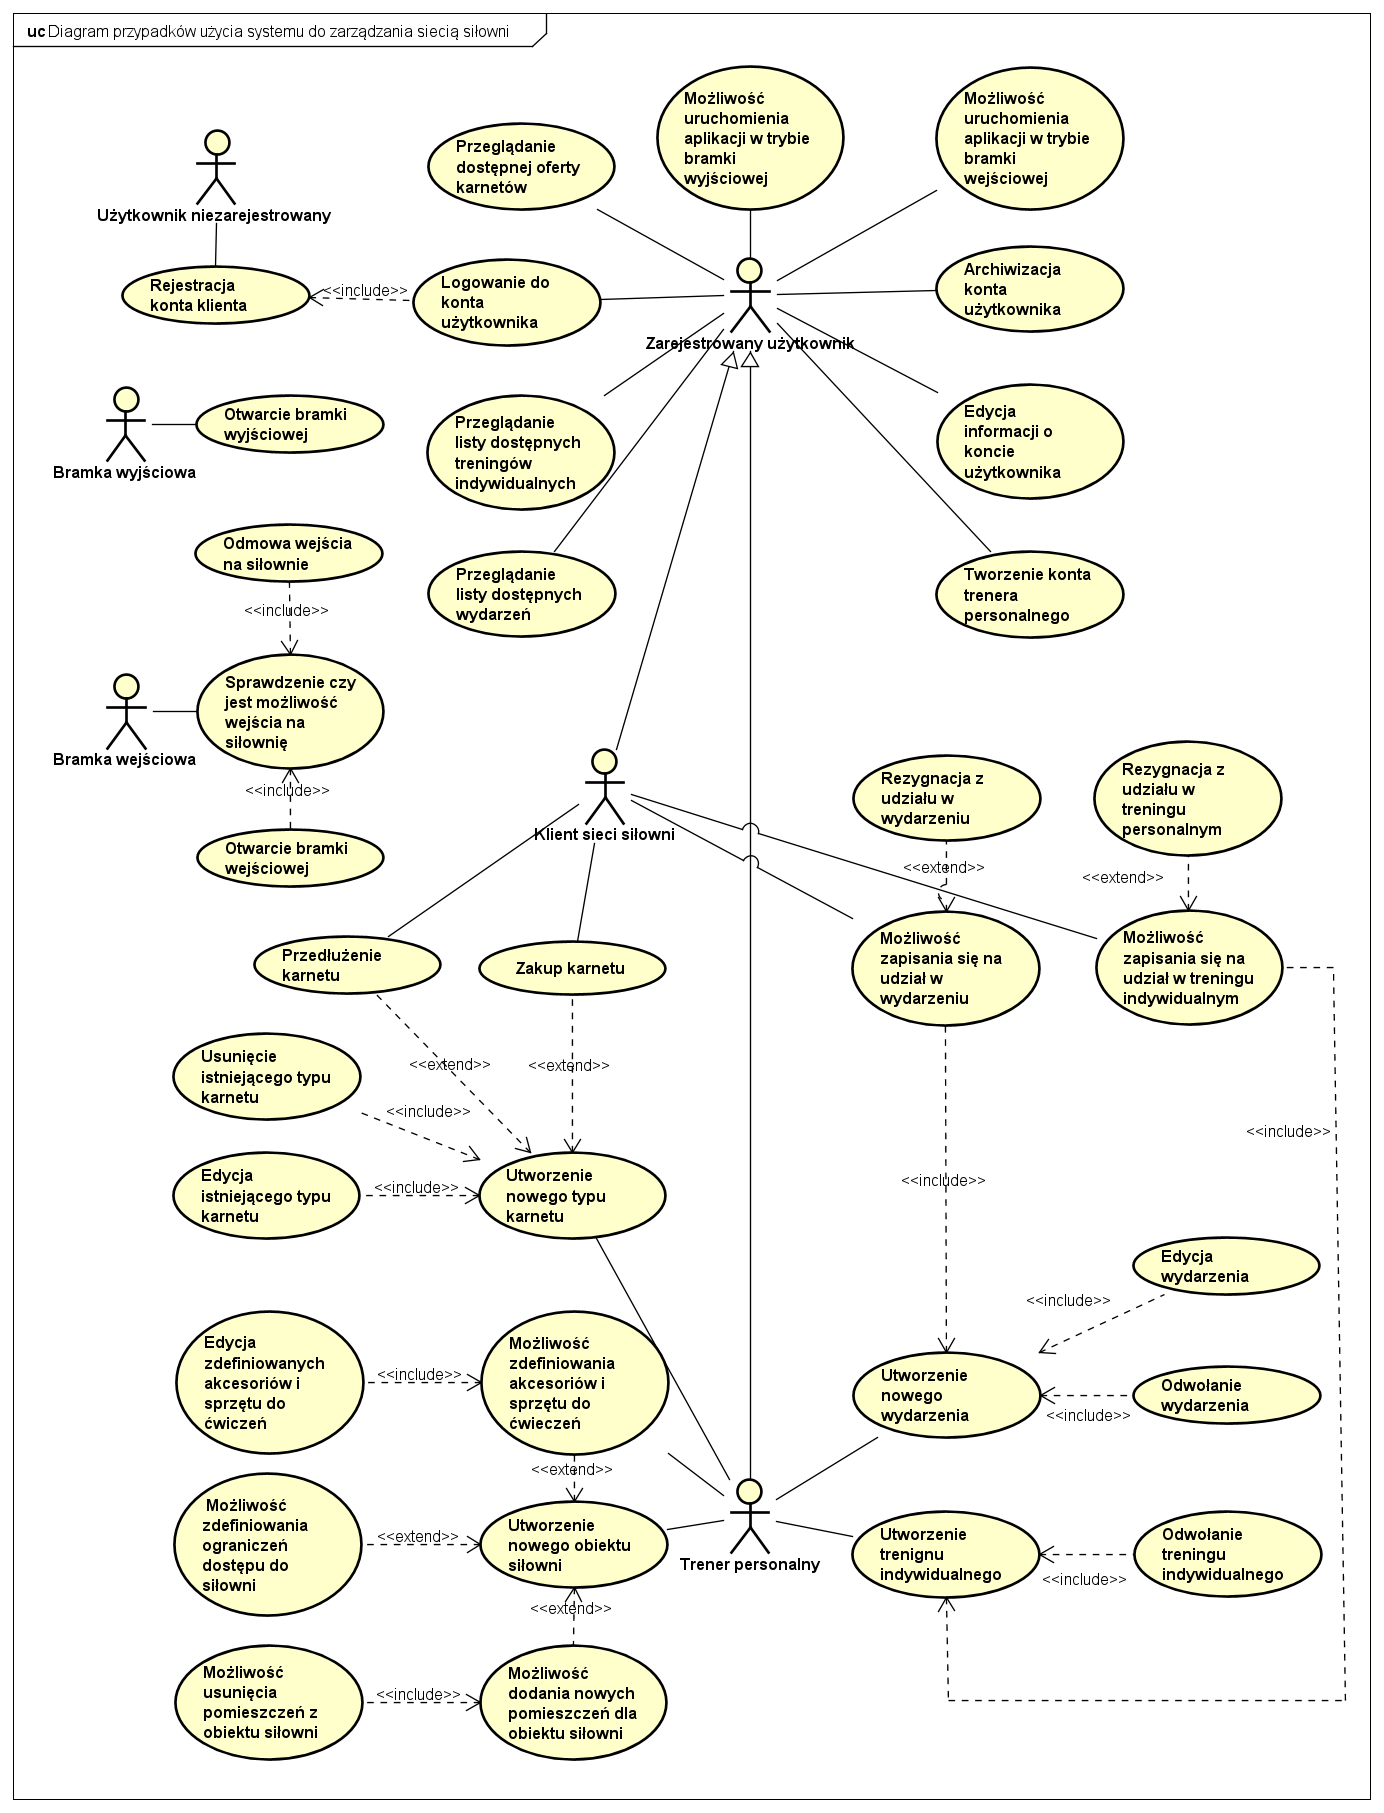
\includegraphics[width=1\linewidth, keepaspectratio]{diagram_przypadków_użycia_xs.png}
	\caption{Diagram przypadków użycia}
	\label{fig:diagramPrzpydakowUzyciaUML}
\end{figure}
	
	\section{Narzędzia}
	Do napisania projektu wykorzystano IDE (ang. \ang{Integrated development environment}) \textit{Visual Studio 2019}, które oferuje wiele narzędzi ułatwiających pisanie kodu w języku \textit{C\#}. Głównymi zaletami tego środowiska jest bliska współpraca z~środowiskiem \textit{.NET}, zapewnienie narzędzi w postaci odpluskwiacza (ang. \ang{debugger}) czy integracja z systemem kontroli wersji GIT. Do pracy wykorzystano również IDE \textit{WebStorm} firmy \textit{JetBrains}, które pozwala na tworzenie aplikacji z~platformą programistyczną \textit{Angular}. Do przeglądania kolekcji i dokumentów w~bazie danych \textit{MongoDB} wykorzystano narzędzie \textit{MongoDB Compass}. Diagramy zostały utworzone dzięki wykorzystaniu narzędzi \textit{Astah UML} i \textit{diagrams.net}.
	
	\section{Wykorzystane zewnętrzne rozwiązania}
	Do projektu zostały wykorzystane nowoczesne platformy programistyczne i biblioteki, które posiadają aktualne wsparcie twórców. Wybrano narzędzia w taki sposób, aby pokryć wymagania funkcjonalne projektu oraz wykorzystać technologie, które są aktualnie wykorzystywane w sposób komercyjny.
	
	Językiem programowania użytym do stworzenia części serwerowej został \textit{C\#} firmy \textit{Microsoft}. Bliskie podobieństwo do języka \textit{Java} oraz wiele usprawnień względem niego pozwala na tworzenie oprogramowania przy wykorzystaniu technik programowania obiektowego, funkcyjnego czy generycznego \cite{bib:csharp}.
	
	Platformą programistyczną warstwy serwerowej została technologia \textit{.NET 5}, która pozwala na tworzenie aplikacji wieloplatformowych z pomocą języka \textit{C\#}. Dzięki użyciu następcy \textit{.NET Core'a}, aplikacja może zostać uruchomiona zarówno na urządzeniach z systemem \textit{Microsoft} jak i dystrybucjach systemu Linux co pozwala na elastyczność względem wyboru środowiska, w którym aplikacja będzie pracować \cite{bib:dotnet5introduction}.
	
	Do stworzenia interfejsu \textit{REST API} została wykorzystana biblioteka \textit{ASP.NET Core}, która pozwala na dodawanie metod interfejsu \textit{REST API}, które będą następnie konsumowane przez warstwę prezentacji. \textit{ASP.NET Core} wspiera wykorzystanie kontenerów wstrzykiwania zależności, obsługę autoryzacji przy pomocy żetonu \textit{JWT} jak i komunikację z wykorzystaniem protokołu HTTPS \cite{bib:asp}.
	
	W celu wykorzystania wzorca projektowego \textit{CQRS} (ang. \ang{command query responsibility separation}) zamiast domyślnego kontenera zależności wykorzystano zewnętrzną bibliotekę \textit{Autofac}, która udostępnia możliwość wstrzykiwania obiektów oznaczonych atrybutami oraz określanie cyklu życia serwisu przy pomocy znaczników \cite{bib:autofactag}.
	
	Wykorzystanie paradygmatu programowania obiektowego prowadziło do potrzeby mapowania niektórych typów na inne. W celu sprawniejszego przeprowadzania takich mapowań wykorzystano bibliotekę \textit{AutoMapper}, która na podstawie podanego obiektu tworzy inny według schematu określonego w klasie profilu (ang. \ang{Profile}).
	
	Jako bazę danych wykorzystano \textit{MongoDB}. \textit{MongoDB} jest dokumentową bazą danych pozwalająca na przechowywanie danych w formacie \textit{JSON}, który jest formatem czytelnym dla człowieka. Baza danych należy do nierelacyjnych baz danych \textit{NoSQL}, której głównymi zaletami są: elastyczny schemat bazy, łatwe skalowanie wszerz oraz możliwość tworzenia zaawansowanych zapytań i raportów\cite {bib:mongodb_guide}. Opcja skalowania bazy wszerz jest istotna w systemach, gdzie trzeba zachować ciągłość działania systemu przy rosnącej bazie użytkowników.
	
	Językiem programowania użytym w części wizualnej aplikacji jest język \textit{TypeScript} zaprojektowany przez firmę \textit{Microsoft}. W odróżnieniu od języka \textit{JavaScript}, \textit{TypeScript} oferuje typowanie w czasie kompilacji, co pozwala na unikanie błędów związanych z niezgodnością typów. Dodanie interfejsów i uogólnień funkcji względem JavaScriptu pozwala na pisanie kodu z wykorzystaniem paradygmatów programowania obiektowego i generycznego \cite {bib:typescript}.
	
	Do stworzenia interfejsu użytkownika została wykorzystana platforma programistyczna Angular, która pozwala na tworzenie aplikacji internetowych przy wykorzystaniu komponentów wielokrotnego użytku. Cechą charakterystyczną platformy jest natywne wykorzystanie języka \textit{TypeScript} oraz możliwość tworzenia aplikacji typu \textit{SPA} \cite{bib:anuglar} \cite{bib:typescript}.
	
	W celu zminimalizowania czasu potrzebnego na tworzenie komponentów warstwy prezentacji wykorzystano bibliotekę \textit{Angular Material} z gotowym zestawem rozwiązań. Kontrolki zawarte w bibliotece implementują filozofię \textit{Google Material} do tworzenia warstw wizualizacji aplikacji internetowych.
	
	W warstwie prezentacji wykorzystano bibliotekę \textit{NgXS}, która pozwala na wykorzystanie wzorca zarządzania stanem. Rozwiązanie implementuje wzorzec projektowy \textit{Redux}, którego główną zaletą jest ułatwienie odpluskwiania warstwy prezentacji oraz zarządzanie danymi poprzez tworzenie stanów (ang. \ang{states}).
	
	\section {Metodyka pracy nad projektowaniem i implementacją}
	
	Prace rozpoczęto od utworzenia osobnych repozytoriów kodu z uwzględnieniem reprezentowanej warstwy aplikacji. Te warstwy to:
	\begin{itemize}
		\item \textit{Samson.Web.Application} - warstwa serwerowa aplikacji. Zawiera kod, który będzie uruchamiany po stronie serwera.
		\item \textit{Samson.Web.Ui} - warstwa prezentacji (ang. \ang{frontend}) aplikacji. Zawiera kod, który będzie uruchamiany na maszynie klienta w celu prezentacji interfejsu użytkownika.
	\end{itemize}

	Następnie podzielono kod warstwy serwerowej na projekty platformy programistycznej .NET. Każdy z projektów został utworzony w taki sposób, aby mógł być zastąpiony w przypadku zmian szczegółów implementacji aplikacji. Podział wygląda następująco:
	\begin{itemize}
		\item \textit{Samson.Web.Application.Api} - projekt zawierający kod kontrolerów platformy ASP.NET, modele wykorzystywane do zapytań HTTP oraz klasy obiektów reprezentujące odpowiedzi serwera na żądania HTTP.
		\item \textit{Samson.Web.Application.Identity} - projekt, który zawiera konfigurację oraz serwisy odpowiedzialne za autoryzację użytkownika.
		\item \textit{Samson.Web.Application.Infrastructure} - projekt posiadający w swojej strukturze utworzone atrybuty, rozszerzenia klas, kod oprogramowania pośredniczącego (ang. \ang middleware) oraz interfejsy wykorzystywane pomiędzy, różnymi projektami rozwiązania .NET.
		\item \textit{Samson.Web.Application.Persistence} - projekt zawierający kod klas implementujących wzorzec repozytorium. Odpowiada za dodawania i modyfikacje encji w bazie danych.
		\item \textit{Samson.Web.Application.ReadModels} - projekt platformy .NET implementujący odczyt z bazy danych.
		\item \textit{Samson.Web.Application.UnitTests} - projekt biblioteki NUnit zawierający kod testów jednostkowych.
		\item \textit{Samson.Web.Application.WebHost} - główny projekt aplikacji. Zawiera konfigurację warstwy serwerowej aplikacji
		\item \textit{Samson.Web.Models} - projekt zawierający modele, wyliczenia (ang. \ang{enum}) oraz modele domenowe aplikacji
	\end{itemize}
	
	W następnych krokach implementowano aplikację tworząc w pierwszej kolejności kontrolery platformy \textit{ASP.NET}, a w krokach późniejszych dodawano szczegóły implementacji w postaci domeny, warstwy zapisu, warstwy odczytu oraz serwisów aplikacyjnych. Najważniejsze klasy domenowe zostały uzupełnione testami jednostkowymi w celu zapewnienia poprawności działania. Gdy tworzenie część serwerowa aplikacji zostało zakończone, rozpoczęto prace nad warstwą interfejsu użytkownika. Warstwa prezentacji była implementowana w następującej kolejności:
	\begin{enumerate}
		\item Opakowanie komponentów z bibliotek zewnętrznych
		\item Utworzenie widoków i formularzy
		\item Integracja z warstwą serwerową
		\item Dodanie obsługi żetonu JWT w komunikacji z warstwą serwerową
	\end{enumerate}

\chapter{Specyfikacja zewnętrzna}
\label{chap:external}
W tym rozdziale znajduje się spis wymagań sprzętowych, których spełnienie jest wymagane do poprawnego działania systemu. W dalszej części znajduje się instrukcja instalacji systemu oraz opis sposobu jego aktywacji. Kolejne podrozdziały opisują kategorie użytkowników i metody, które zostały wykorzystane do zabezpieczenia wrażliwych danych. Rozdział kończy się przykładami działania aplikacji w postaci zrzutów ekranu i opisów.

\section {Wymagania sprzętowe}
Aby aplikacja działała w poprawny sposób spełnione muszą być poniższe wymagania:
	\begin{itemize}
		\item System operacyjny w wersji \cite{bib:requirementsWin} \cite{bib:requirementsMac} \cite{bib:requirementsLinux} \cite{bib:requirementsMongo} \cite{bib:requirementsFramework}:
		\begin {itemize}
			\item \textit{Windows} w wersjach 11/10/8.1
			\item \textit{Windows 7} z \textit{Service Pack 1}
			\item \textit{Windows Server Core 2012 R2}
			\item Nano Server w wersji nowszej niż 1809
			\item \textit{MacOS} 12.0 \textit{Monterey}
			\item \textit{MacOS} 11.0 \textit{Big Sur}
			\item \textit{MacOS} 10.15 \textit{Catalina}
			\item \textit{Linux Alpine} w wersji nowszej niż 3.12 włącznie
			\item \textit{Linux CentOS} w wersjach 8/7
			\item \textit{Linux Debian} w werjsach 11/10/9
			\item \textit{Linux Fedora} w wersjach 35/34/33/32
			\item \textit{Linux OpenSuse} w wersji 15
			\item \textit{Linux RedHat} w wersjach 8/7
			\item \textit{Linux SLES} w wersji 15
			\item \textit{Linux Ubuntu} w wersjach 21.10/21.04/20.04
		\end {itemize}	
		\item Procesor z więcej niż jednym rdzeniem o taktowaniu nie mniejszym niż 1 GHz
		\item Pamięć operacyjna większa niż 4 GB RAM
		\item Minimalna przestrzeń na dysku to 4,5 GB pamięci
		\item Zainstalowana nowoczesna przeglądarka WWW taka jak:
		\begin{itemize}
			\item \textit{Google Chrome} w najnowszej wersji
			\item \textit{Mozilla Firefox} w najnowszej wersji
			\item \textit{Microsoft Edge} w najnowszej wersji
			\item \textit{Opera} w najnowszej wersji
		\end{itemize}
	\end{itemize}

Są to minimalne wymagania do uruchomienia bazy danych \textit{MongoDB} oraz aplikacji z wykorzystaniem platformy uruchomieniowej \textit{.NET 5}. Ponadto wymagane są dodatkowe zasoby potrzebne do uruchomienia przeglądarki, w której wyświetlony zostanie interfejs użytkownika.

\section {Instalacja}

\subsection{Instalacja bazy danych MongoDB}
W celu zainstalowania aplikacji, trzeba spełnić wymagania wymienione w poprzednim punkcie. Instalacja zostaje rozpoczęta od pobrania i zainstalowania serwera bazy danych \textit{MongoDB} w wersji Community \href{https://www.mongodb.com/try/download/community}{z strony twórców}.
\begin{figure}[h!]
	\centering
	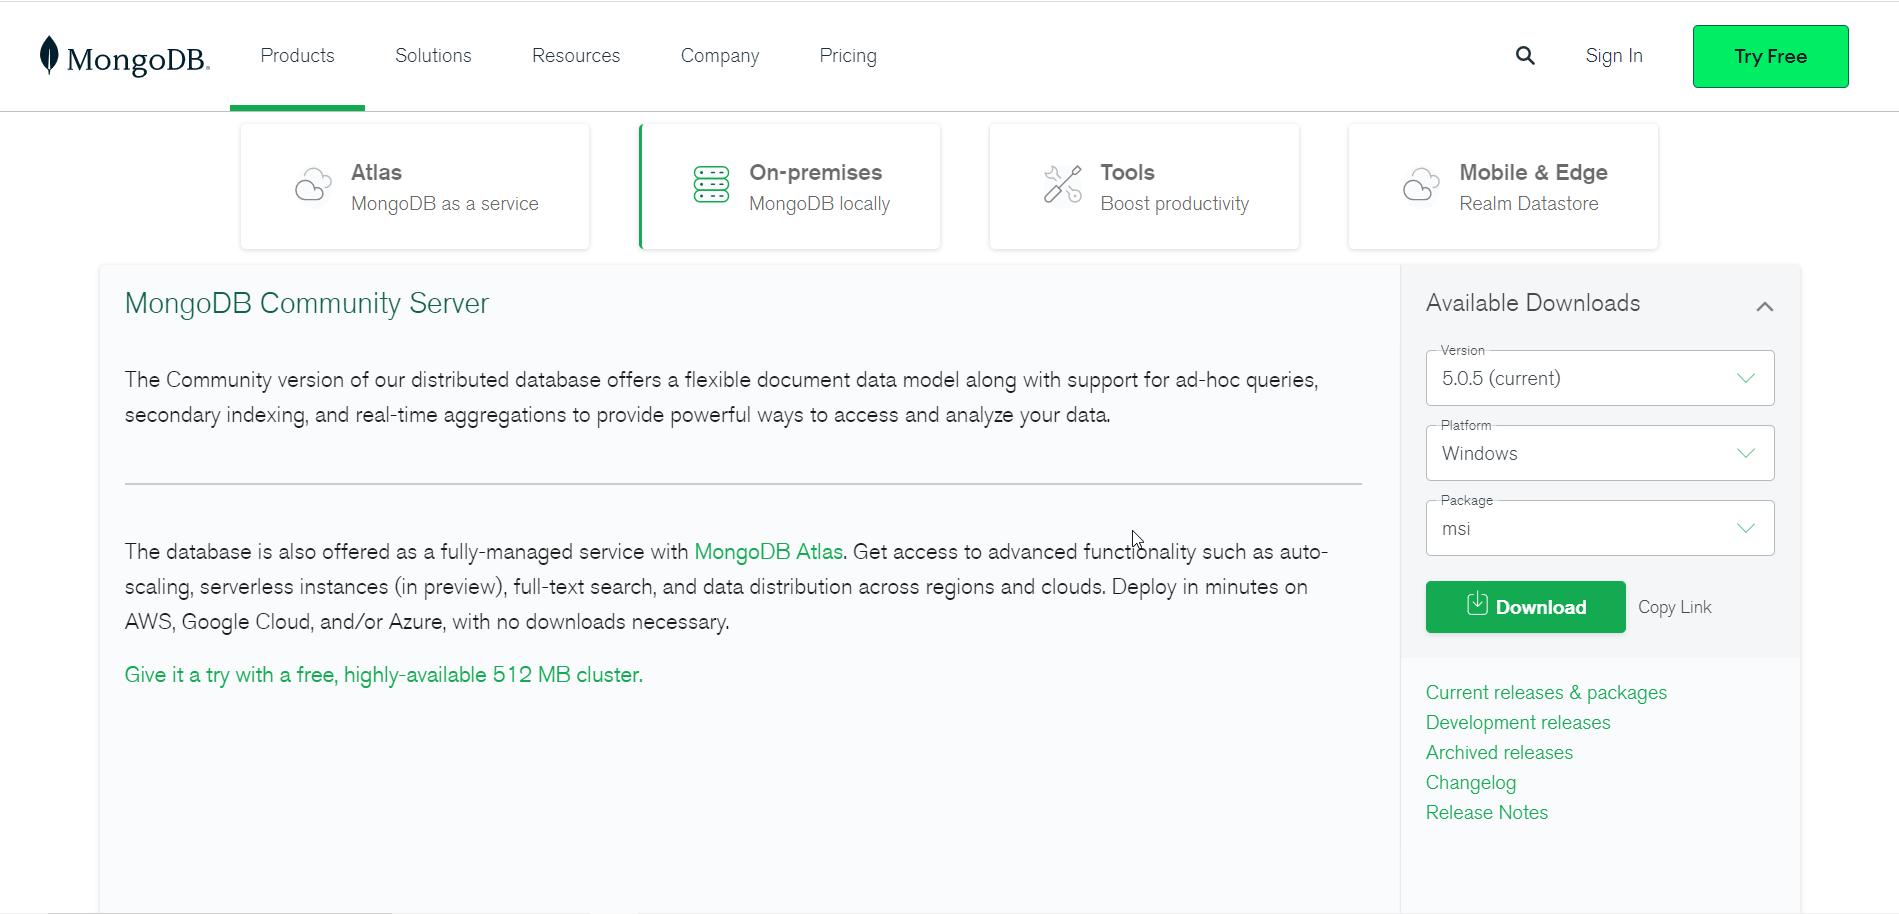
\includegraphics[width=1\linewidth]{../zrzuty_ekranu/instalcja_mongodb/mongodbsite}
	\caption{Strona, z której można pobrać instalator serwera bazy danych MongoDB}
	\label{fig:mongodbsite}
\end{figure}
\FloatBarrier

Instalacja oprogramowania do zarządzania bazą danych rozpoczyna się od uruchomienia wcześniej pobranego kreatora.
\begin{figure}[h!]
	\centering
	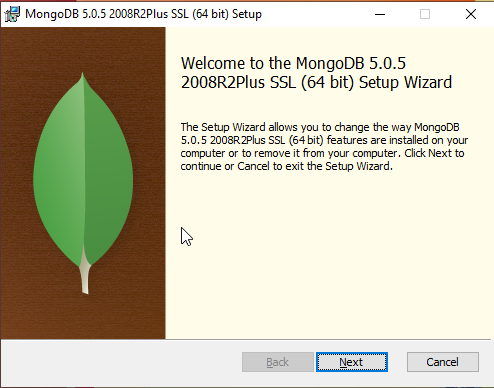
\includegraphics[width=0.75\linewidth]{../zrzuty_ekranu/instalcja_mongodb/mongodb1}
	\caption{Widok powitalny instalatora MongoDB}
	\label{fig:mongodb1}
\end{figure}
\FloatBarrier

\newpage
Po zapoznaniu się z warunkami licencyjnymi, aby kontynuować użytkownik musi zaznaczyć pole z podpisem \textit{I accept the terms in the License Agreement}, a~następnie przycisnąć \textit{Next}.
\begin{figure}[h!]
	\centering
	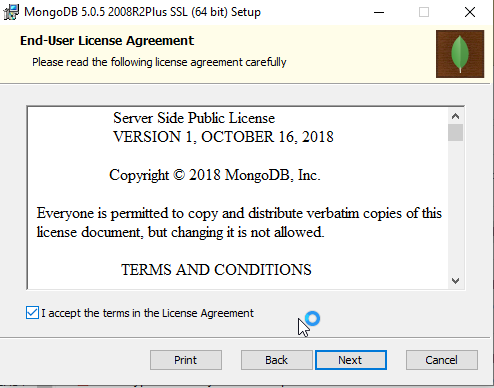
\includegraphics[width=0.65\linewidth]{../zrzuty_ekranu/instalcja_mongodb/mongodb2}
	\caption{Umowa licencyjna \textit{MongoDB Community Edition}}
	\label{fig:mongodb2}
\end{figure}
\FloatBarrier

W widoku formularza wyboru typu instalacji trzeba wybrać opcję \textit{Completed}, aby zainstalować wszystkie potrzebne narzędzia do działania serwera.
\begin{figure}[h!]
	\centering
	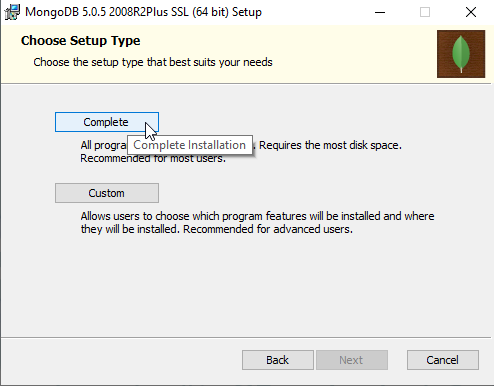
\includegraphics[width=0.6\linewidth]{../zrzuty_ekranu/instalcja_mongodb/mongodb3}
	\caption{Typ instalacji w instalatorze \textit{MongoDB Community Edition}}
	\label{fig:mongodb3}
\end{figure}
\FloatBarrier

W następnym widoku, gdzie widać konfiguracje serwera, ustawienia powinny zostać domyślne.
\begin{figure}[h!]
	\centering
	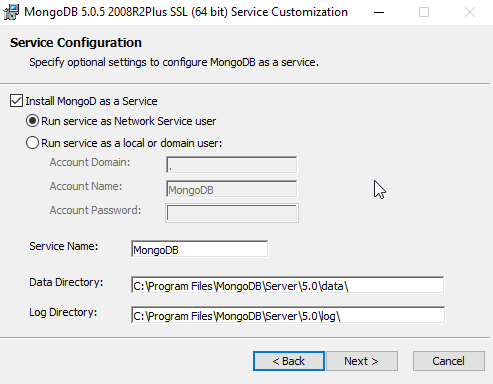
\includegraphics[width=0.6\linewidth]{../zrzuty_ekranu/instalcja_mongodb/mongodb4}
	\caption{Początkowa konfiguracja serwera bazy danych}
	\label{fig:mongodb4}
\end{figure}
\FloatBarrier

Po naciśnięciu przycisku \textit{Next} powinna być widoczna opcja zainstalowania \textit{MongoDB Compass}. Oprogramowanie \textit{MongoDB Compass} jest opcjonalne, więc opcja instalacji może zostać odznaczona.
\begin{figure}[h!]
	\centering
	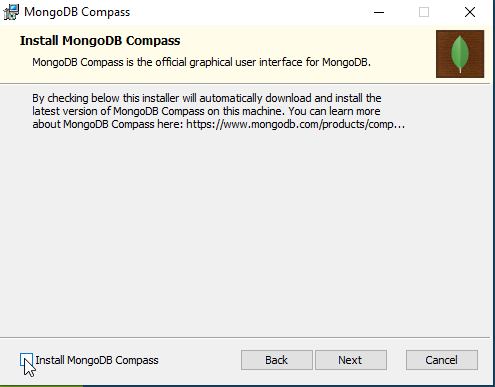
\includegraphics[width=0.6\linewidth]{../zrzuty_ekranu/instalcja_mongodb/mogndodb5}
	\caption{Informacja o możliwości instalacji klienta bazy danych \textit{MongoDB Compass}}
	\label{fig:mogndodb5}
\end{figure}
\FloatBarrier

\newpage
W następnym kroku, aby zainstalować serwer bazy danych trzeba nacisnąć przycisk \textit{Install}.
\begin{figure}[h!]
	\centering
	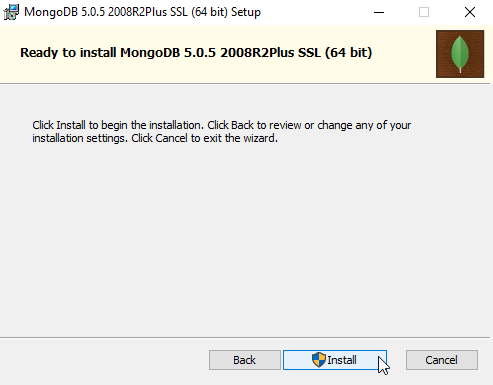
\includegraphics[width=0.6\linewidth]{../zrzuty_ekranu/instalcja_mongodb/mongodb6}
	\caption{Rozpoczęcie instalacji \textit{MongoDB}}
	\label{fig:mongodb6}
\end{figure}
\FloatBarrier

Aby zakończyć działanie kreatora po zakończeniu się procesu instalacji trzeba przycisnąć przycisk \textit{Finish}. W tym momencie na maszynie użytkownika powinna znajdować się zainstalowana bazy danych \textit{MongoDB}.
\begin{figure}[h!]
	\centering
	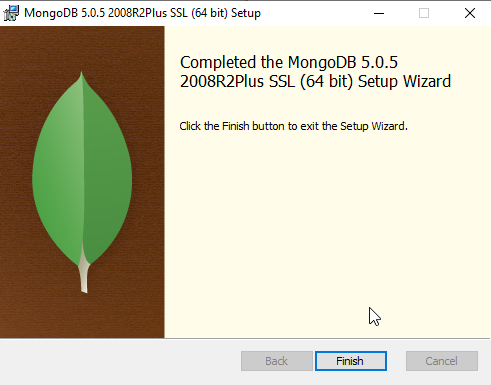
\includegraphics[width=0.65\linewidth]{../zrzuty_ekranu/instalcja_mongodb/mongodb_finish}
	\caption{Zakończenie instalacji \textit{MongoDB}}
	\label{fig:mongodbfinish}
\end{figure}
\FloatBarrier

\subsection{Instalacja środowiska .NET 5}
Podobnie jak w przypadku \textit{MongoDB}, aby zainstalować środowisko \textit{.NET 5} trzeba przejść na \href{https://dotnet.microsoft.com/en-us/download/dotnet/5.0}{stronę, gdzie możliwe jest pobranie \textit{SDK .NET 5}}. W pierwszej kolejności wymagane jest wybranie odpowiedniej wersji instalatora dla zainstalowanego systemu operacyjnego oraz architektury maszyny.
\begin{figure}[h!]
	\centering
	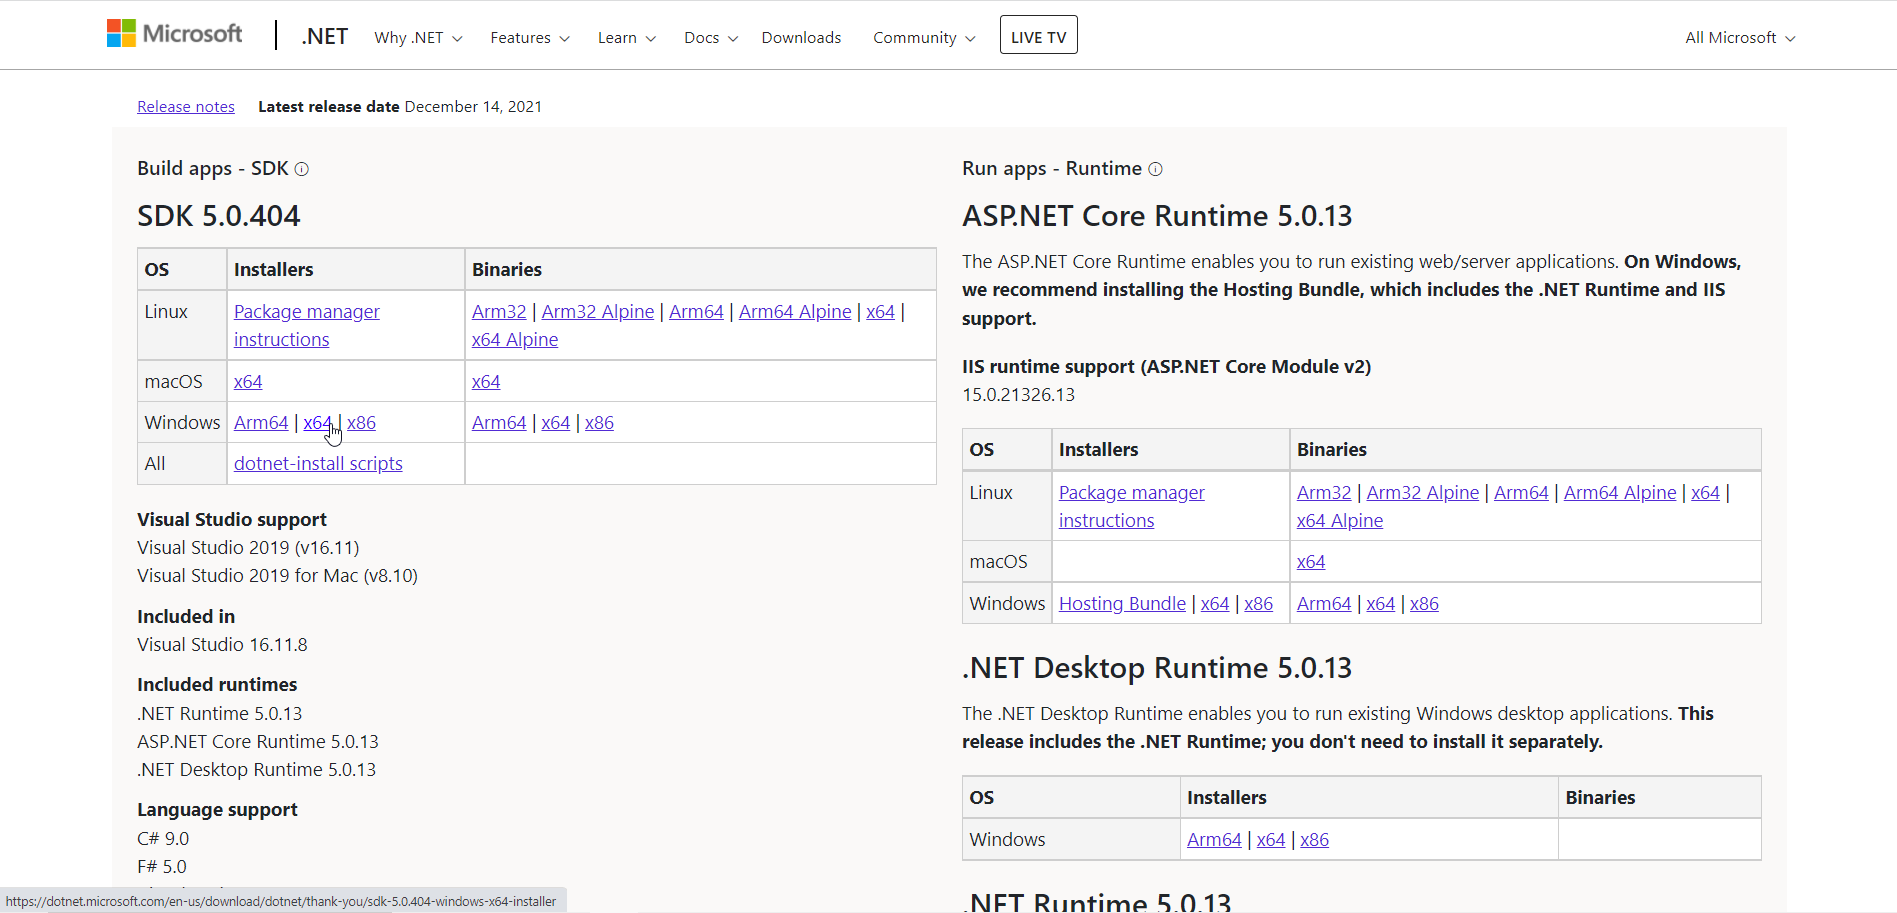
\includegraphics[width=1\linewidth]{../zrzuty_ekranu/instalacja_dotnet5/dotnet_sdk}
	\caption{Strona twórców środowiska \textit{.NET}}
	\label{fig:dotnetsdk}
\end{figure}
\FloatBarrier

W kolejnym kroku trzeba uruchomić pobrany kreator instalacji \textit{SDK .NET 5}. Pierwszym widokiem jest formularz informujący o dostępnej dokumentacji oraz składnikach instalacji. Po zapoznaniu się z informacji trzeba przycisnąć przycisk \textit{Zainstaluj} w celu instalacji środowiska uruchomieniowego.
\begin{figure}[h!]
	\centering
	
\includegraphics[width=0.7\linewidth]{../zrzuty_ekranu/instalacja_dotnet5/dotnet1}
	\caption{Rozpoczęcie instalacji środowiska \textit{.NET }5}
	\label{fig:dotnet1}
\end{figure}
\FloatBarrier

Następnie kreator zainstaluje na maszynie wymagane składniki. Kiedy działanie instalatora dobiegnie końca, użytkownik powinien zamknąć kreator przy pomocy przycisku \textit{Zamknij}.

\begin{figure}[h!]
	\centering
	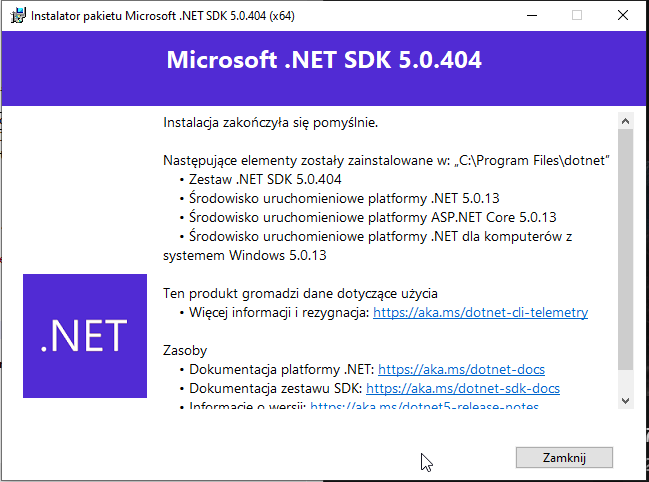
\includegraphics[width=0.7\linewidth]{../zrzuty_ekranu/instalacja_dotnet5/dotnet_finish}
	\caption{Zakończenie instalacji środowiska \textit{.NET 5}}
	\label{fig:dotnetfinish}
\end{figure}
\FloatBarrier

Aby sprawdzić czy instalacja przebiegła pomyślnie trzeba uruchomić konsolę \textit{Windows Powershell} dla systemów rodziny \textit{Windows} lub odpowiedniego terminala dla posiadanej dystrybucji \textit{Linux}. Następnie trzeba wpisać komendę \textit{dotnet --version}. Jeśli instalacja przebiegła pomyślnie użytkownik powinien zobaczyć w~konsoli informację o zainstalowanej wersji środowiska \textit{.NET}.

\subsection{Instalacja środowiska Node.js}
Przedostatnim krokiem, jaki trzeba wykonać, aby zainstalować projekt jest instalacja środowiska, które pozwoli na uruchomienie serwera WWW dzięki, któremu będzie można uruchomić aplikację stworzoną przy pomocy platformy programistycznej Angular. Serwer WWW musi mieć możliwość przekierowania wszystkich zapytań do wybranego adresu URL. Jest to istotne w przypadku aplikacji typu \textit{SPA}, gdzie to aplikacja odpowiada za nawigacje pomiędzy widokami. W tej pracy zaprezentowana zostanie instalacja serwera \textit{http-server}, który obsługuje takie przekierowania.

W pierwszej kolejności zainstalowana musi być platforma uruchomieniowa \textit{Node.js}, która pozwala na wykonywanie skryptów napisanych w języku \textit{JavaScript}. Kreator instalacji można pobrać z strony twórców \href{https://nodejs.org/en/}{środowiska}.
\begin{figure}[H]
	\centering
	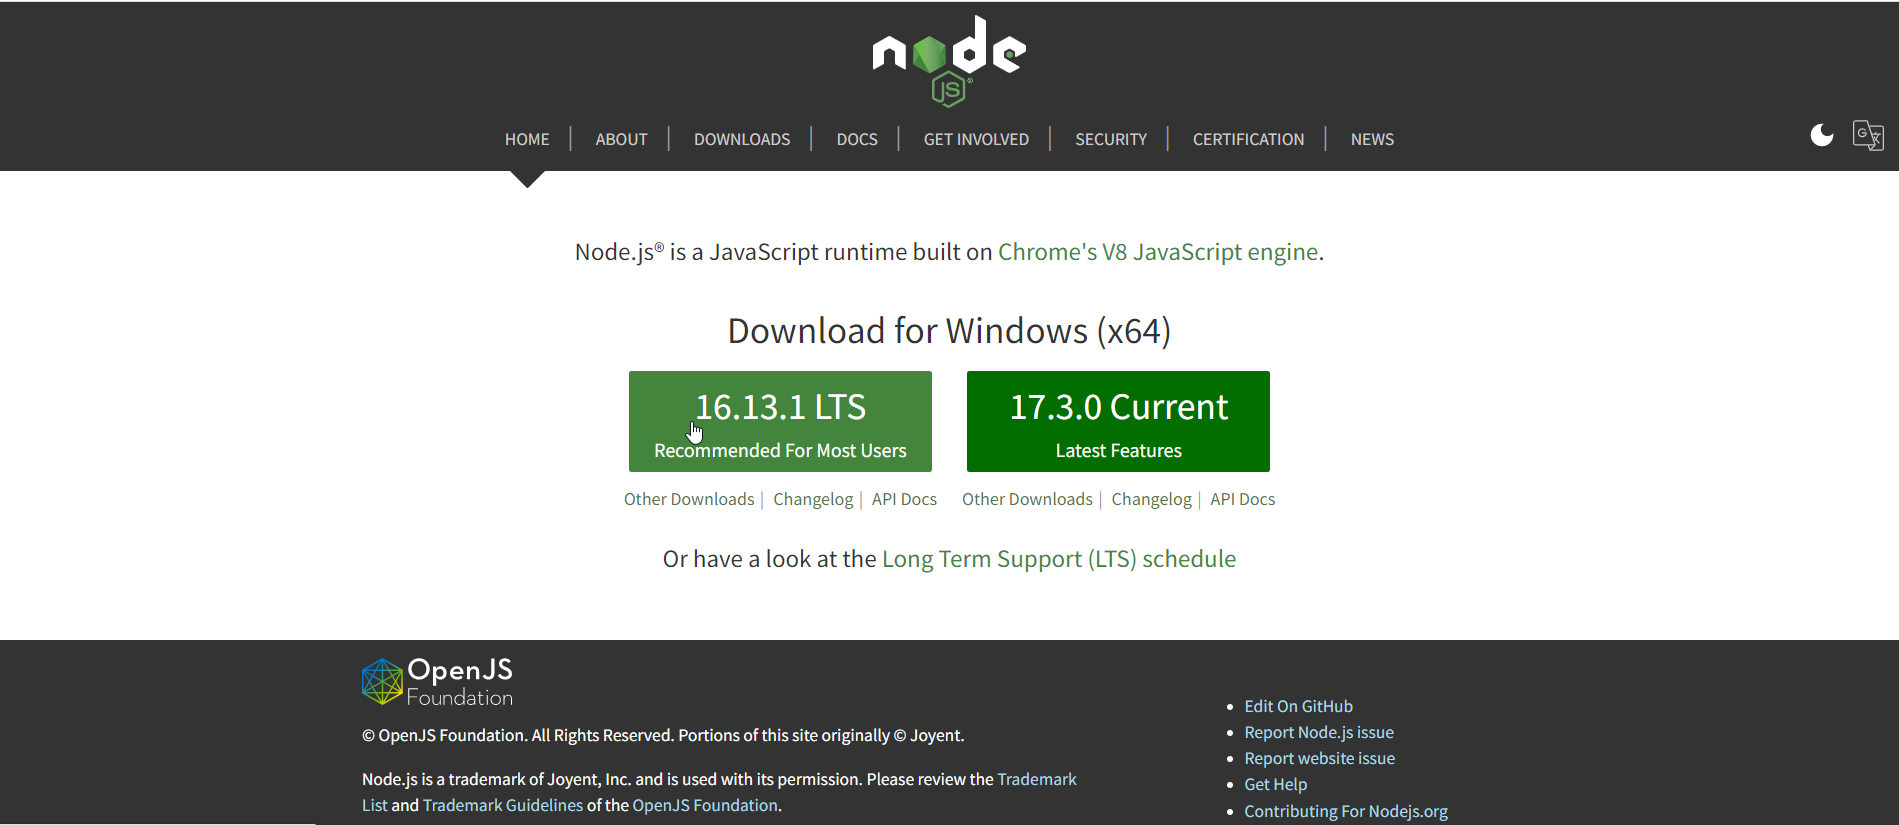
\includegraphics[width=0.8\linewidth]{../zrzuty_ekranu/instalacja_nodejs/node_page}
	\caption{Strona Node.js}
	\label{fig:nodepage}
\end{figure}

Kolejnym krokiem jest uruchomienie programu instalującego środowisko uruchomieniowe. Aby to zrobić trzeba przejść do lokalizacji na dysku gdzie pobrano plik instalatora a następnie uruchomić go. Wyświetlony powinien zostać następujący widok.
\begin{figure}[h!]
	\centering
	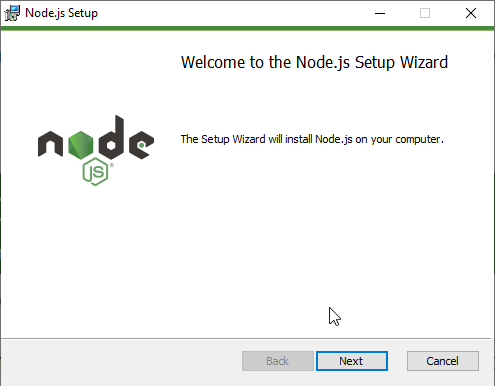
\includegraphics[width=0.65\linewidth]{../zrzuty_ekranu/instalacja_nodejs/node1}
	\caption{Rozpoczęcie instalacji środowiska \textit{Node.js}}
	\label{fig:node1}
\end{figure}
\FloatBarrier

Po przyciśnięciu przycisku \textit{Next} oczom użytkownika powinien ukazać się formularz z informacjami o licencji oprogramowania. Aby przejść dalej użytkownik powinien zapoznać sie z licencją a następnie zaakceptować ją. Po zaakceptowaniu licencji użytkownik musi przejść do kolejnego widoku za pomocą przycisku \textit{Next}.
\begin{figure}[h!]
	\centering
	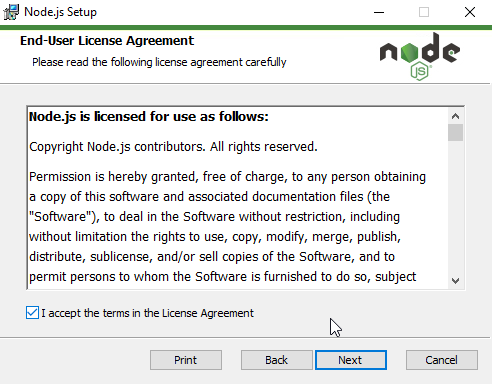
\includegraphics[width=0.65\linewidth]{../zrzuty_ekranu/instalacja_nodejs/node2}
	\caption{Licencja środowiska \textit{Node.js}}
	\label{fig:node2}
\end{figure}
\FloatBarrier

\newpage
Następnym etapem instalacji jest wybór ścieżki do folderu, gdzie ma zostać zainstalowane oprogramowanie. Po wyborze dogodnej lokalizacji trzeba przejść do kolejnego widoku.
\begin{figure}[h!]
	\centering
	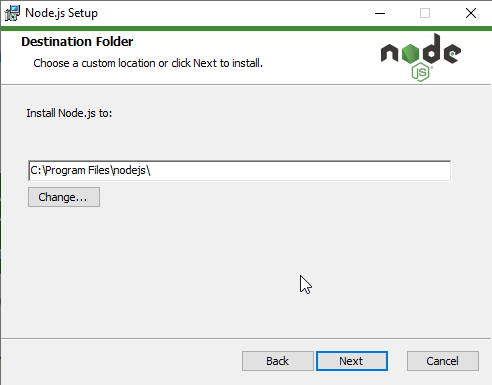
\includegraphics[width=0.6\linewidth]{../zrzuty_ekranu/instalacja_nodejs/node3}
	\caption{Ścieżka do folderu docelowego \textit{Node.js}}
	\label{fig:node3}
\end{figure}


W kolejnym kroku użytkownik musi wybrać składniki instalacji. W tym przypadku pozostać powinny domyślne opcje. Istotne jest aby zainstalowane zostało narzędzie \textit{NPM}, które pozwoli na instalacje serwera WWW.
\begin{figure}[h!]
	\centering
	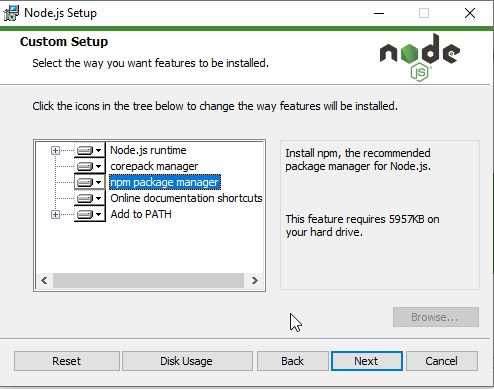
\includegraphics[width=0.6\linewidth]{../zrzuty_ekranu/instalacja_nodejs/node4}
	\caption{Składniki instalatora Node.js}
	\label{fig:node4}
\end{figure}
\FloatBarrier

Jednym z ostatnich kroków instalatora jest widok z informacją o możliwości zainstalowania dodatkowego narzędzia \textit{Chocolatey}. Narzędzie to nie jest potrzebne do działania, więc można wyłączyć opcję instalacji narzędzia.
\begin{figure}[h!]
	\centering
	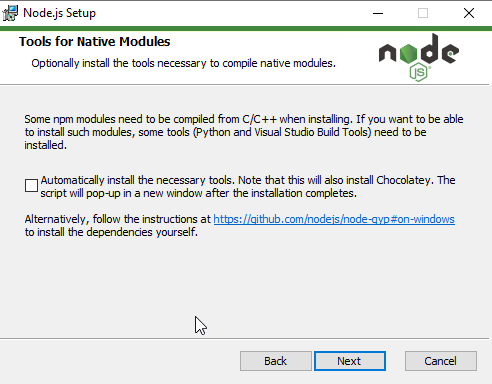
\includegraphics[width=0.6\linewidth]{../zrzuty_ekranu/instalacja_nodejs/node5}
	\caption{Formularz umożliwiający instalację dodatkowego narzędzia \textit{Cocolatey}}
	\label{fig:node5}
\end{figure}
\FloatBarrier

W kolejnych etapach instalacji użytkownik powinien uruchomić instalacje za pomocą przycisku \textit{Install}. Po zakończonej instalacji instalator powinien wyświetlić informację o zakończeniu pracy.
\begin{figure}[h!]
	\centering
	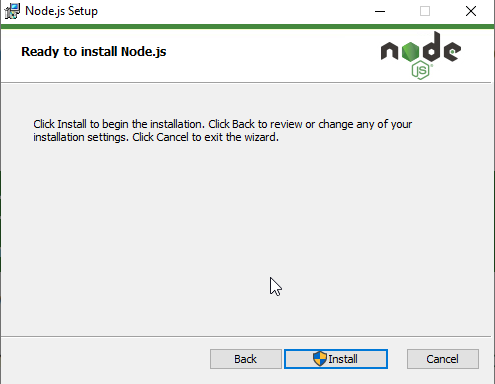
\includegraphics[width=0.55\linewidth]{../zrzuty_ekranu/instalacja_nodejs/node6}
	\caption{Potwierdzenie instalacji środowiska \textit{Node.js}}
	\label{fig:node6}
\end{figure}
\FloatBarrier

Aby sprawdzić czy instalacja przebiegła pomyślnie, można uruchomić polecenie \textit{node -v}, które powinno zwrócić informację o zainstalowanej wersji \textit{Node.js}.

\subsection {Instalacja \textit{http-server}}
Ostatnim etapem instalacji systemu jest instalacja serwera WWW, który obsługuje możliwość przekierowań do pliku \textit{index.html}. Aby zainstalować serwer \textit{http-server} w terminalu trzeba uruchomić polecenie zaprezentowane na Kod \ref{lst:httpServerInstall}.
\begin{lstlisting}[caption={Instalacja paczki \textit{http-server}}, label={lst:httpServerInstall}]
	npm install -g http-server
\end{lstlisting}

Polecenie to zainstaluje paczkę \textit{npm} do użytku w obrębie całego systemu. Dzięki instalacji globalnej użytkownik będzie mógł uruchomić serwer WWW z każdej lokalizacji na dysku.

\section {Sposób aktywacji}
\subsection{Uruchomienie warstwy serwerowej}
Aby uruchomić aplikację stworzoną z wykorzystaniem platformy \textit{.NET} istnieje potrzeba skompilowania jej do pliku wykonywalnego. W celu utworzenia pliku \textit{exe} użytkownik musi przejść do folderu, w którym znajduje się projekt \textit{Samson.Web.Application}, a następnie z poziomu terminala wywołać komendę pokazaną na Kod \ref{lst:dotnetCompilation}.
\begin{lstlisting}[caption={Kompilacja projektu \textit{ASP.NET}}, label={lst:dotnetCompilation}]
	dotnet restore;
	dotnet build --configuration Release
\end{lstlisting}
Pierwsza z komend wymusza instalację zewnętrznych zależności, które są zawarte w postaci paczek \textit{NuGet'owych}. Paczki te pozwalają na udostępnianie kodu napisanego przy wykorzystaniu platformy \textit{.NET}, a następnie mogą zostać wykorzystane do innych projektów przy pomocy narzędzia \textit{NuGet}. Druga komenda buduje projekt i zwraca wynik w postaci dynamicznych bibliotek \textit{dll} i pliku wykonywalnego \textit{exe}.

W folderze \textit{./Samson.Web.Application.WebHost/bin/Release/net5.0} powinien powstać folder zawierający wyniki kompilacji. Następnie w celu uruchomienia pliku wykonywalnego użytkownik powinien przejść do folderu \\ ./Samson.Web.Application.WebHost/bin/Release/net5.0 przy pomocy komendy zaprezentowanej na Kod \ref{lst:aspnetChangeFolder}.
\begin{lstlisting}[caption={Przejście do folderu zawierającego plik wykonywalny}, label={lst:aspnetChangeFolder}]
	cd ./Samson.Web.Application.WebHost/bin/Release/net5.0
\end{lstlisting}

Aby uruchomić warstwę serwerową aplikacji wymagane jest dodanie odpowiednich zmiennych środowiskowych przy pomocy polecenia pokazanego na Kod \ref{lst:varEnvironment}. Przeznaczenie zmiennych jest następujące:
\begin{itemize}
	\item \textit{MongoDB:DatabaseName} - nazwa bazy danych jaka zostanie utworzona w~środowisku \textit{MongoDB}.
	\item \textit{Authentication:JWT:Key} - klucz wykorzystywany do funkcji mieszającej, która jest wykorzystywana do zabezpieczenia żetonu \textit{JWT}.
	\item \textit{ASPNETCORE\_ENVIRONMENT} - oznaczenie typu środowiska. Nie powinna zostać zmieniana.
	\item \textit{ConnectionString:MongoDB:Atlas} - ciąg znaków określający parametry połączenia z bazą danych. Jeżeli w trakcie instalacji serwera \textit{MongoDB} wartości domyślnie nie zostały zmienione to proponowany ciąg znaków powinien pozwolić na poprawne połączenie z bazą danych.
\end{itemize}
Wartości parametrów mogą zostać zmodyfikowane, ale zalecane jest aby pozostały w niezmienionej formie ze względu na proponowaną w wcześniejszych krokach konfigurację.
\begin{lstlisting}[caption={Ustawienie wartości zmiennych środowiskowych}, label={lst:varEnvironment}]
	$env:MongoDB:DatabaseName="SamsonDatabase";
	$env:Authentication:JWT:Key="Top secret key to provide JWT token";
	$env:ASPNETCORE_ENVIRONMENT="Release"
	$env:ConnectionString:MongoDB:Atlas="mongodb://localhost:27017/?readPreference=primary&ssl=false";
\end{lstlisting}

Ostatnim krokiem w uruchomieniu warstwy serwerowej jest uruchomienie polecenia przedstawionego na Kod \ref{lst:aspNetRun}.
\begin{lstlisting}[caption={Uruchomienie warstwy serwerowej aplikacji}, label={lst:aspNetRun}]
	start Samson.Web.Application.WebHost.exe
\end{lstlisting}

\subsection{Uruchomienie warstwy prezentacji}
Tak jak w przypadku warstwy serwerowej, warstwa prezentacji musi zostać skompilowana do postaci, która może zostać obsłużona przez serwer WWW. Aby to zrobić trzeba uruchomić terminal a następnie przejść do lokalizacji, w której znajduje się projekt \textit{Samson.Web.Ui}. Kolejnym krokiem jest wywołanie poleceń, które zainstalują wymagane zależności a następnie utworzą paczkę wynikową. Polecenia zostały wypisane na Kod \ref{lst:installAndBuildAngularProejct}.
\begin{lstlisting}[caption={Polecenie, które tworzy paczkę możliwą do uruchomienia przez serwer WWW}, label={lst:installAndBuildAngularProejct}]
	npm install; npm run build
\end{lstlisting}

Końcowym krokiem uruchamiania warstwy interfejsu użytkownika jest uruchomienie serwera WWW z opcją przekierowania do pliku \textit{index.html}. Polecenie zostało przedstawione na Kod \ref{lst:runWWWServer}.
\begin{lstlisting}[caption={Polecenie, które tworzy paczkę możliwą do uruchomienia przez serwer WWW}, label={lst:runWWWServer}]
	cd dist/samson-web-ui; http-server --proxy http://localhost:8080?
\end{lstlisting}

Po wywołaniu poprzedniego polecania aplikacja internetowa powinna być dostępna pod adresem: \textit{http://localhost:8080}.

\section {Kategorie użytkowników}

Aplikacja internetowa kategoryzuje użytkowników na dwie kategorie:
\begin{itemize}
	\item Trenerów personalnych - pełnią rolę administratorów \ref{UseExample}ystemie. Posiadają możliwość modyfikacji zasobów siłowni, takich jak sprzęt do ćwiczeń, obiekty siłowni, pomieszczeń oraz możliwość organizacji wydarzeń i treningów indywidualnych.
	\item Klientów - użytkownicy którzy posiadają możliwość zakupu karnetu , zgłoszenia chęci udziału w treningu indywidualnym lub wydarzeniu.
\end{itemize}

\section {Kwestie bezpieczeństwa}

System wykorzystuje żeton bezpieczeństwa \textit{JWT}. Żeton ten generowany jest w części serwerowej aplikacji w trakcie logowania użytkownika. Kiedy użytkownik poprawnie zaloguje się do systemu, serwer przesyła żeton do warstwy interfejsu użytkownika, gdzie zostaje zapisany w \textit{localstorage} przeglądarki. Warstwa prezentacji dodaje za każdym razem żeton do nagłówka żądania protokołu HTTP, które będzie wymagało uwierzytelnienia użytkownika. W momencie gdy warstwa serwerowa otrzyma taki żeton sprawdza zapisane w nim dane o jego terminie ważności i dostępach, które posiada użytkownik. Jeśli użytkownik systemu posiada odpowiednie uprawnienia do zasobu to otrzymuje odpowiedź na żądanie, w przeciwnym razie system zwraca informacje o błędzie oznaczone statusem 401 (Unauthorized). Brak przesłania żetonu w nagłówku do metody wymagającej autoryzacji skończy się za każdym razem błędem oraz informacją o próbie nieautoryzowanego dostępu do wrażliwych danych.

\section {Przykład działania}
\label{UseExample}
W tej części pracy zaprezentowano przykładowe scenariusze działania systemu. Prezentowane są one z perspektywy różnych użytkowników, ze względu na różnice w posiadanych uprawnieniach.

\subsection{Rejestracja i logowanie}
Jako pierwsze zaprezentowane zostanie logowanie i rejestracja w systemie. Są to jedne z początkowych widoków jakie zobaczy użytkownik korzystając z systemu.
\subsubsection{Rejestracja}
Rejestracja pozwala na utworzenie, konta klienta. Konto daje dostęp do systemu i jego możliwości.
\begin{figure}[h!]
	\centering
	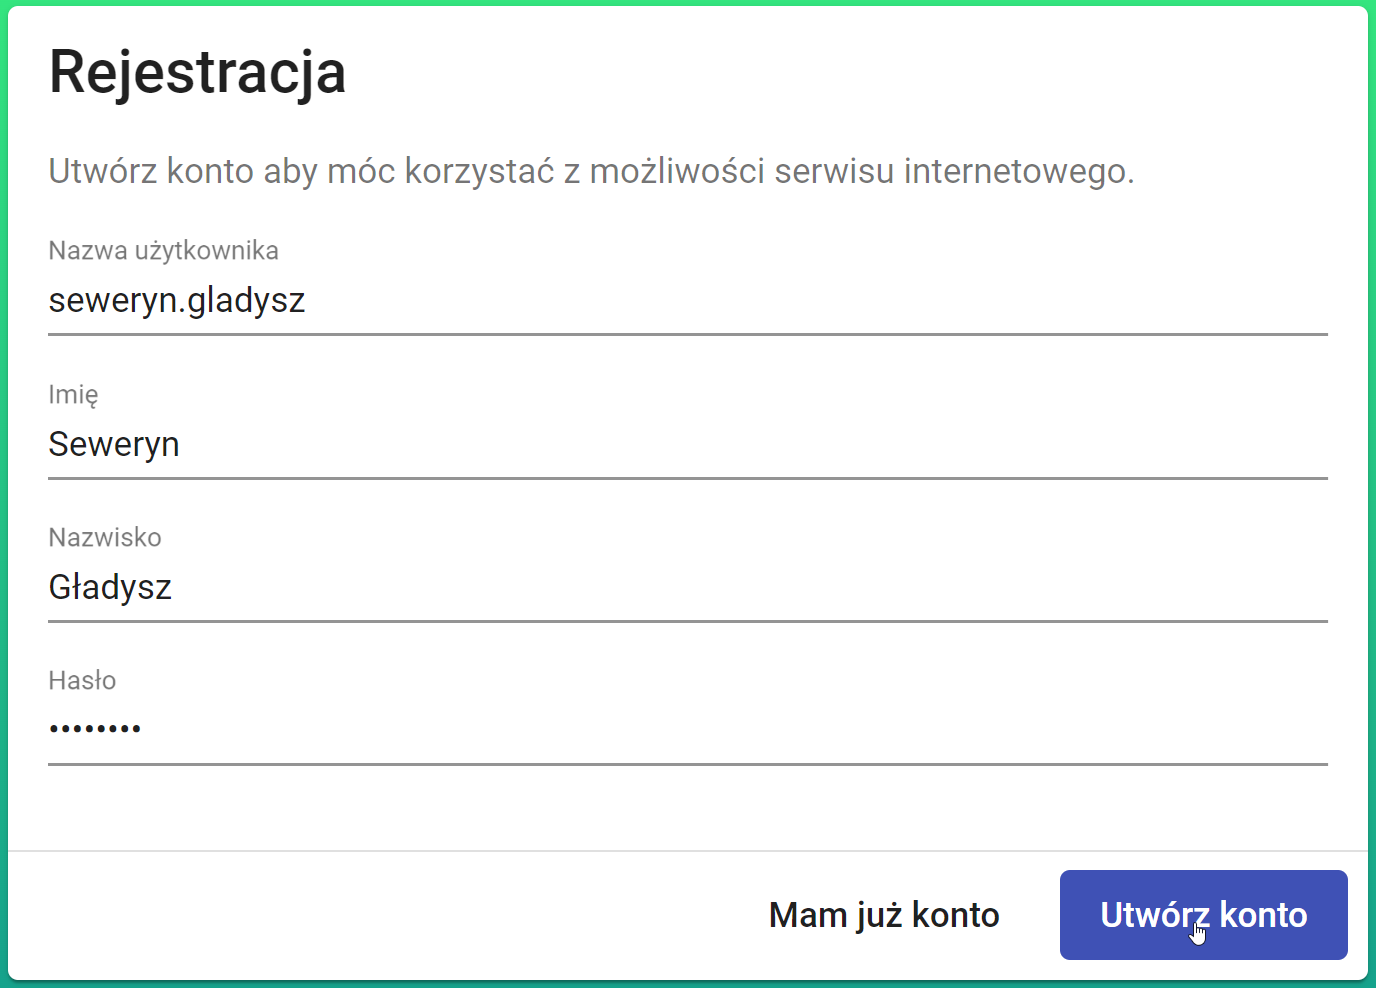
\includegraphics[width=1\linewidth]{../zrzuty_ekranu/dzialanie/rejestracja_logowanie/rejestracja}
	\caption{Rejestracja klienta}
	\label{fig:rejestracja}
\end{figure}
\FloatBarrier
Jeżeli użytkownik wypełni wszystkie wymagane dane oraz wybierze nazwę konta, która nie została wcześniej wykorzystana przez innego użytkownika to powinien zobacz informację o poprawnie utworzonym koncie.
\begin{figure}[h!]
	\centering
	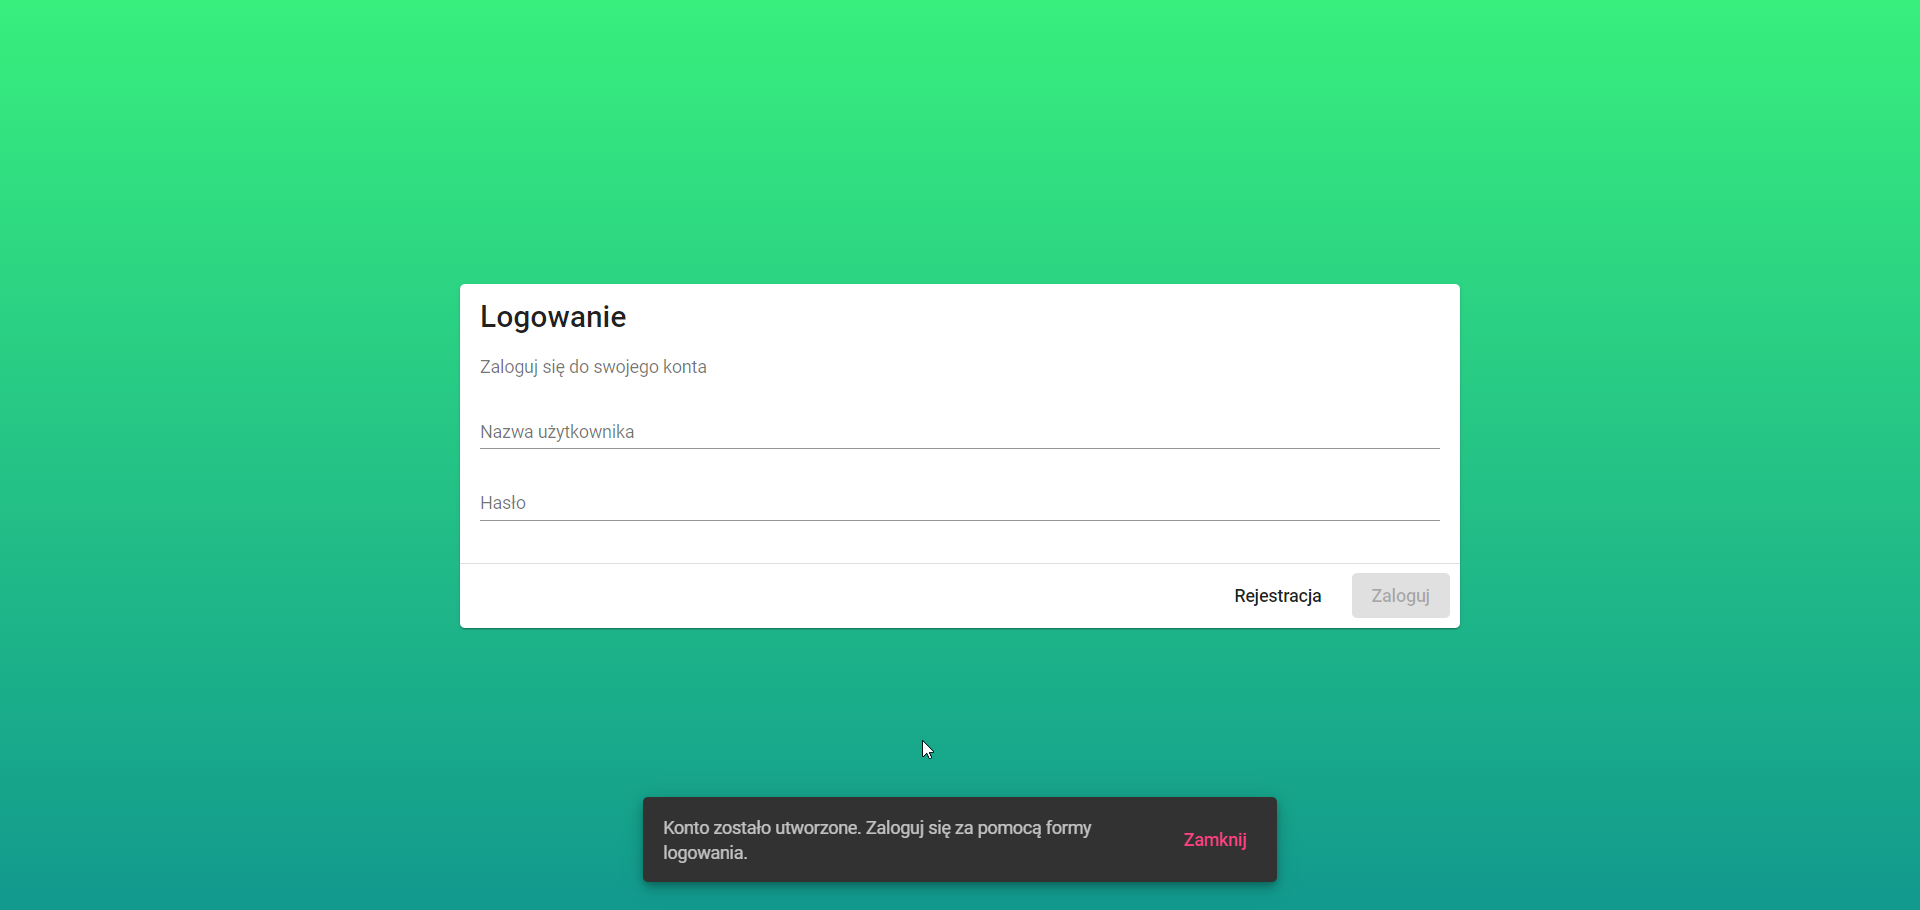
\includegraphics[width=0.7\linewidth]{../zrzuty_ekranu/dzialanie/rejestracja_logowanie/konto_utworzone}
	\caption{Klient został zarejestrowany w systemie}
	\label{fig:kontoutworzone}
\end{figure}
\FloatBarrier

\subsubsection{Logowanie}
Klient i trener personalny ma możliwość zalogowania się do systemu w celu skorzystania z jego funkcjonalności.
\begin{figure}[h!]
	\centering
	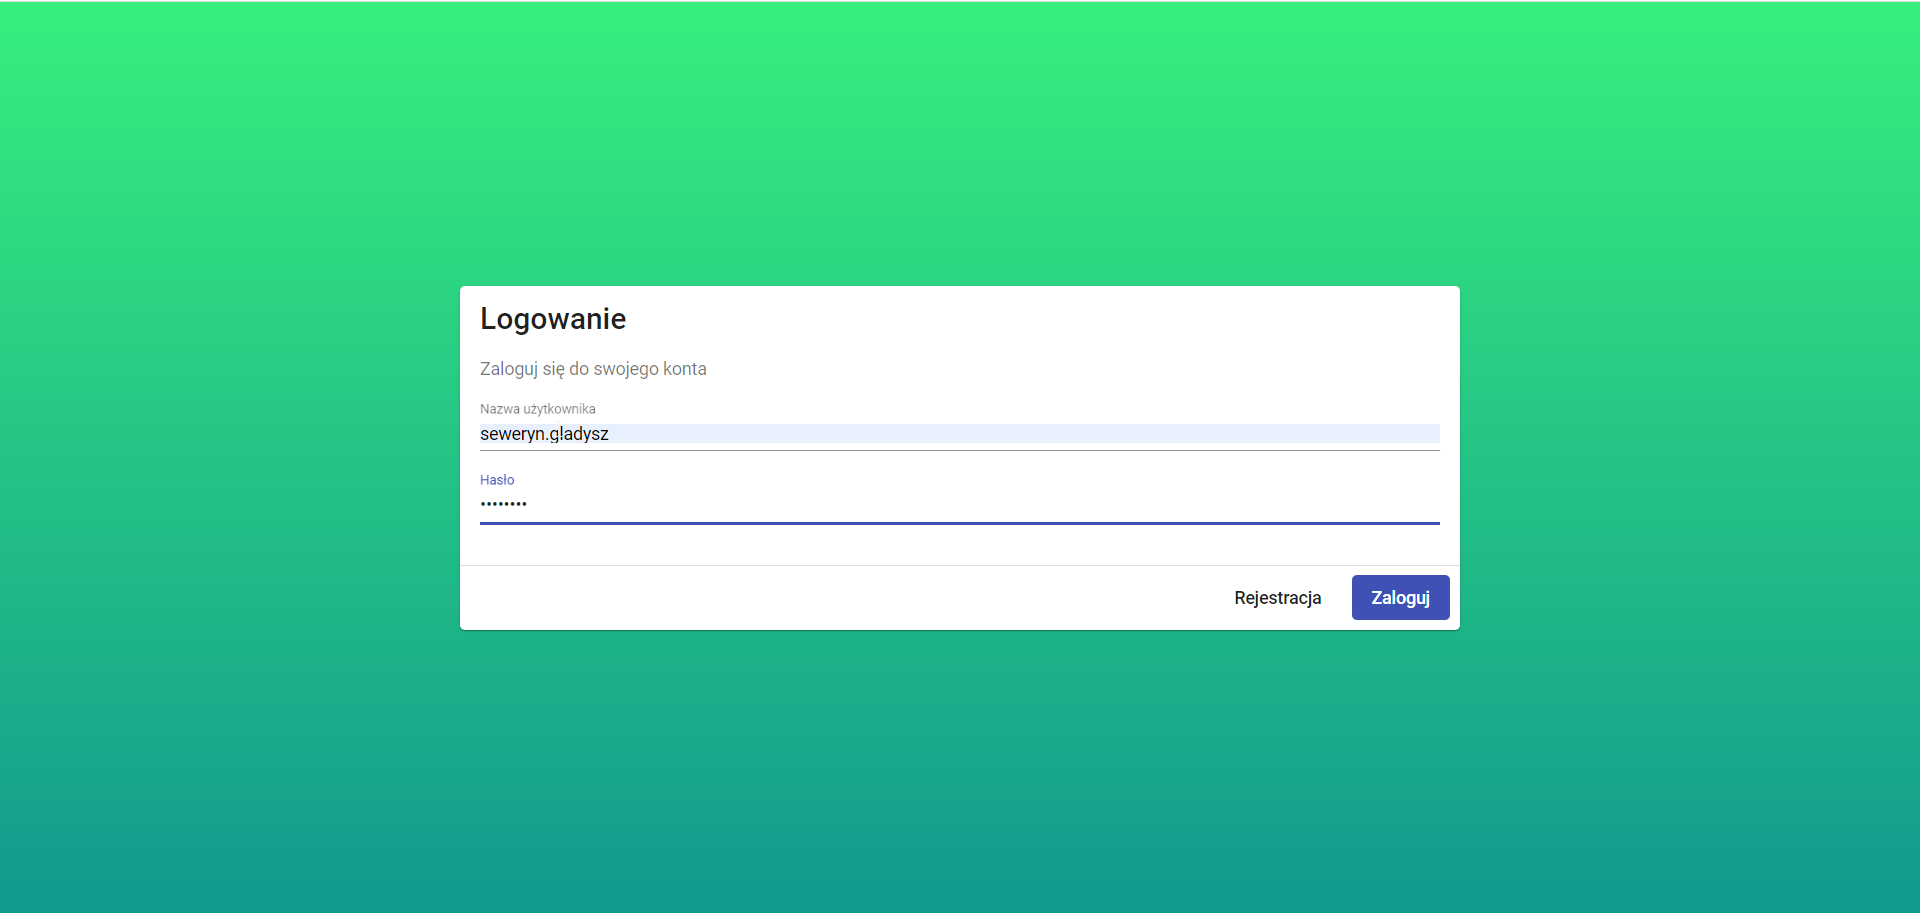
\includegraphics[width=0.75\linewidth]{../zrzuty_ekranu/dzialanie/rejestracja_logowanie/logowanie}
	\caption{Widok logowania do systemu}
	\label{fig:logowanie}
\end{figure}
\FloatBarrier
Użytkownik zostanie zalogowany jeśli wypełni w sposób poprawny dane w formularzu logowania.
\begin{figure}[h!]
	\centering
	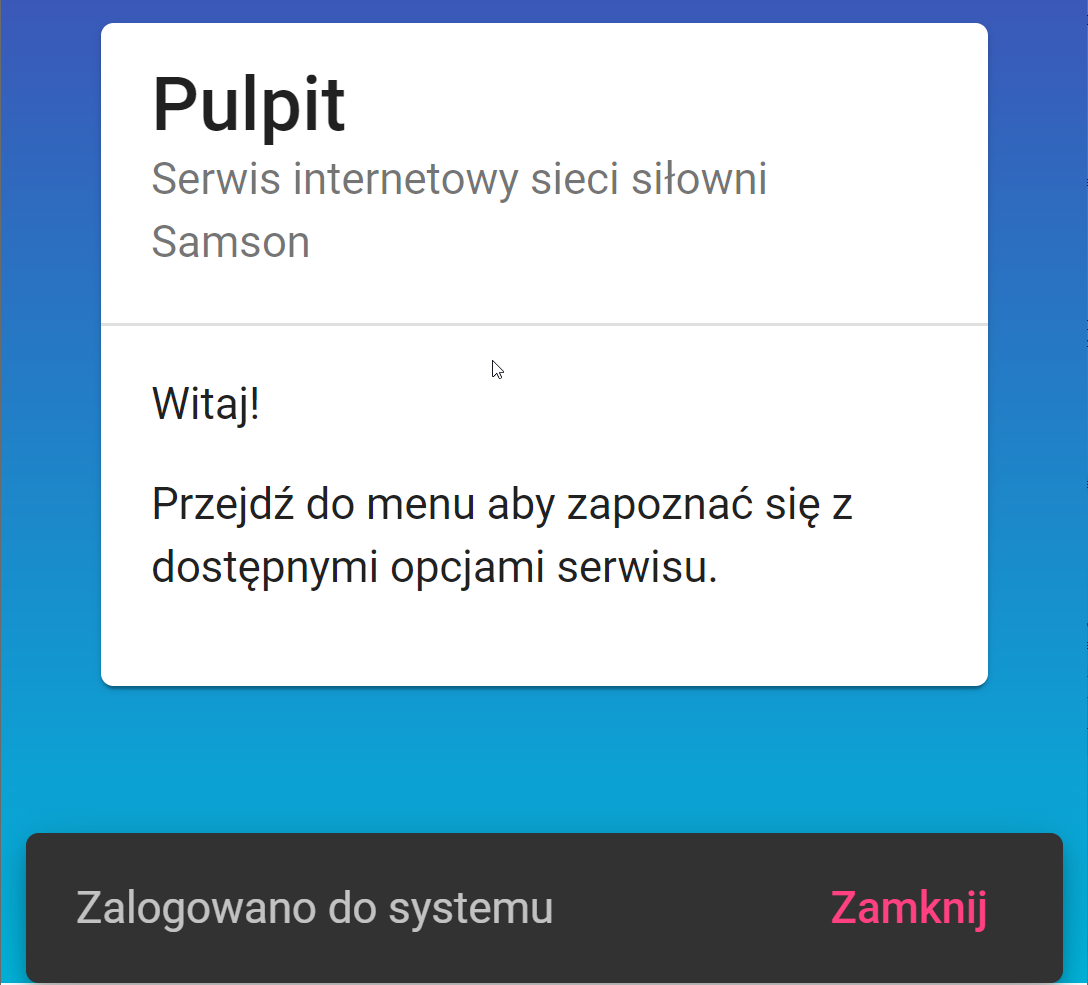
\includegraphics[width=0.75\linewidth]{../zrzuty_ekranu/dzialanie/rejestracja_logowanie/zalogowano}
	\caption{Widok po zalogowaniu do systemu}
	\label{fig:zalogowano}
\end{figure}
\FloatBarrier

\subsection{Administracja systemem}
System powinien udostępniać możliwość zarządzania systemem oraz zasobami sieci siłowni przy jego pomocy. Aplikacja pozwala na zarządzanie obiektami siłowni, pomieszczeniami, które do tych obiektów zostały przypisane, sprzętem do ćwiczeń, akcesoriami oraz ofertą karnetów.

\subsubsection{Dodawanie konta trenerów personalnych}
Użytkownik ma możliwość utworzenia konta trenera personalnego.
\begin{figure}[h!]
	\centering
	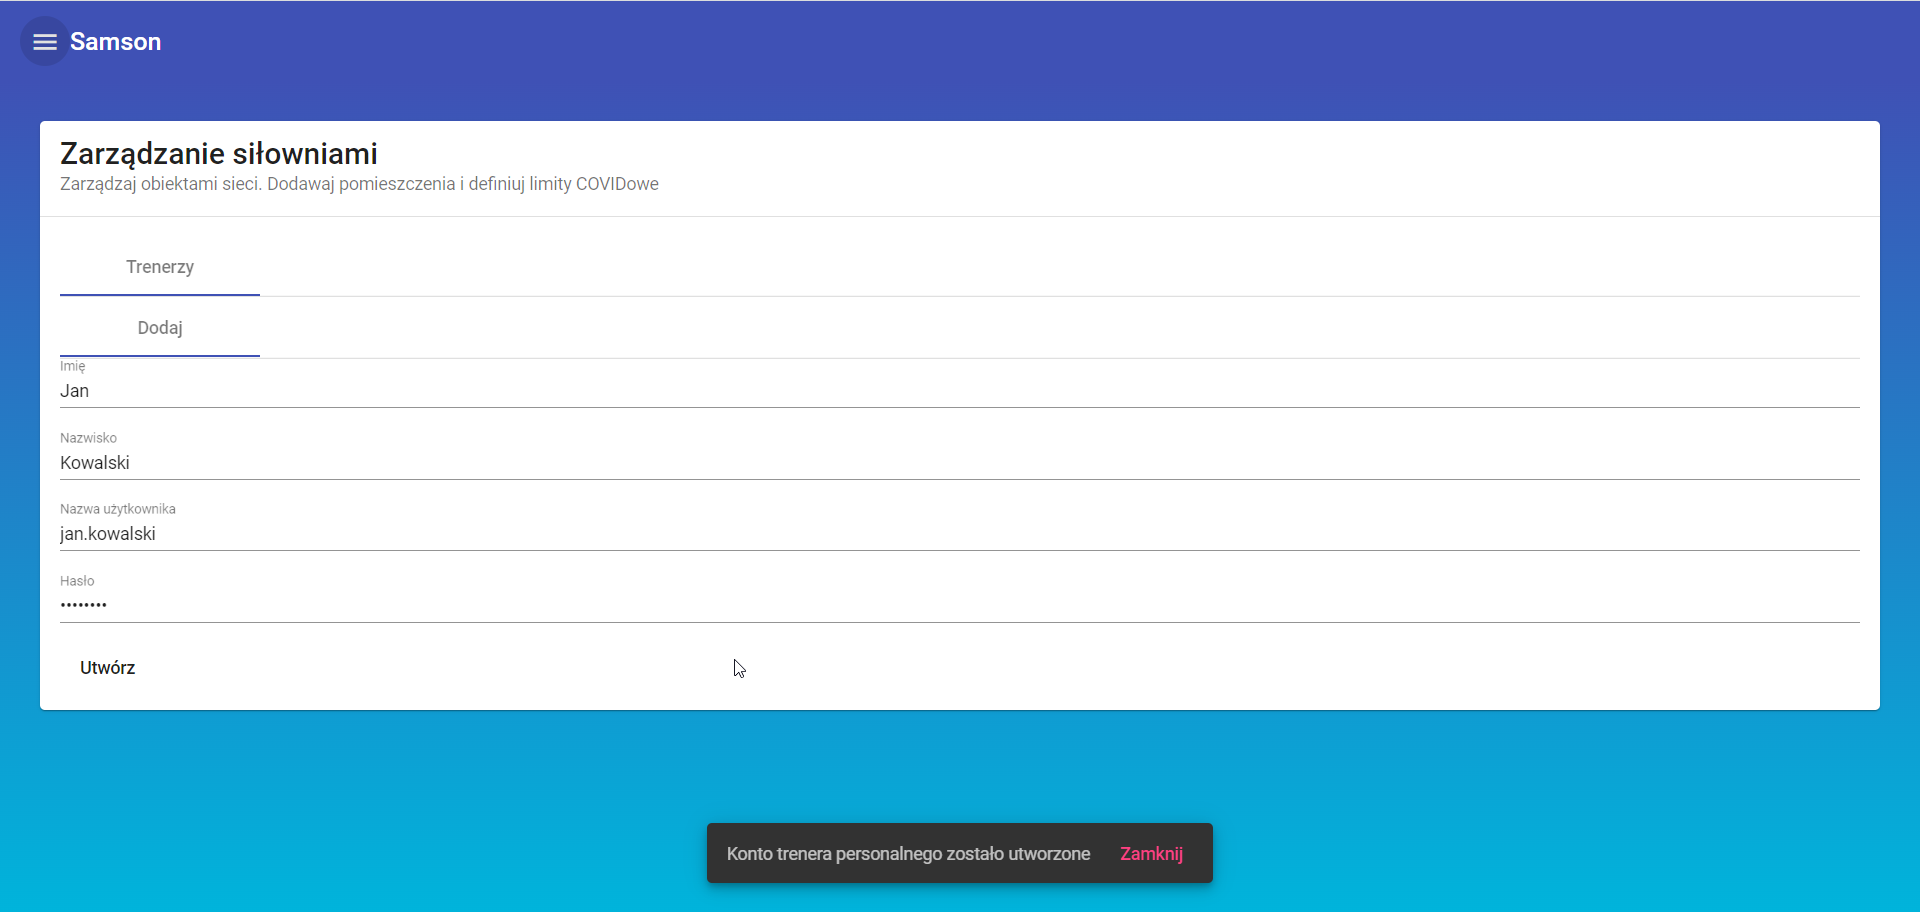
\includegraphics[width=0.5\linewidth]{../zrzuty_ekranu/dzialanie/trener_personalny/tworzenie_konta_trenera_personalnego}
	\caption{Formularz tworzenia konta trenera personalnego}
	\label{fig:tworzeniekontatrenerapersonalnego}
\end{figure}
\FloatBarrier

\subsubsection{Zarządzanie obiektami siłowni}
Trenerzy personalni pełnią rolę administratorów, co pozwala im na zarządzanie obiektami siłowni.
W pierwszej kolejności utworzony zostanie nowy obiekt sieci siłowni. W trakcie procesu dodawania obiektu wymagane jest, aby podana została nazwa oraz ilość osób jaka może przebywać na jednym metrze kwadratowym siłowni.
\begin{figure}[h!]
	\centering
	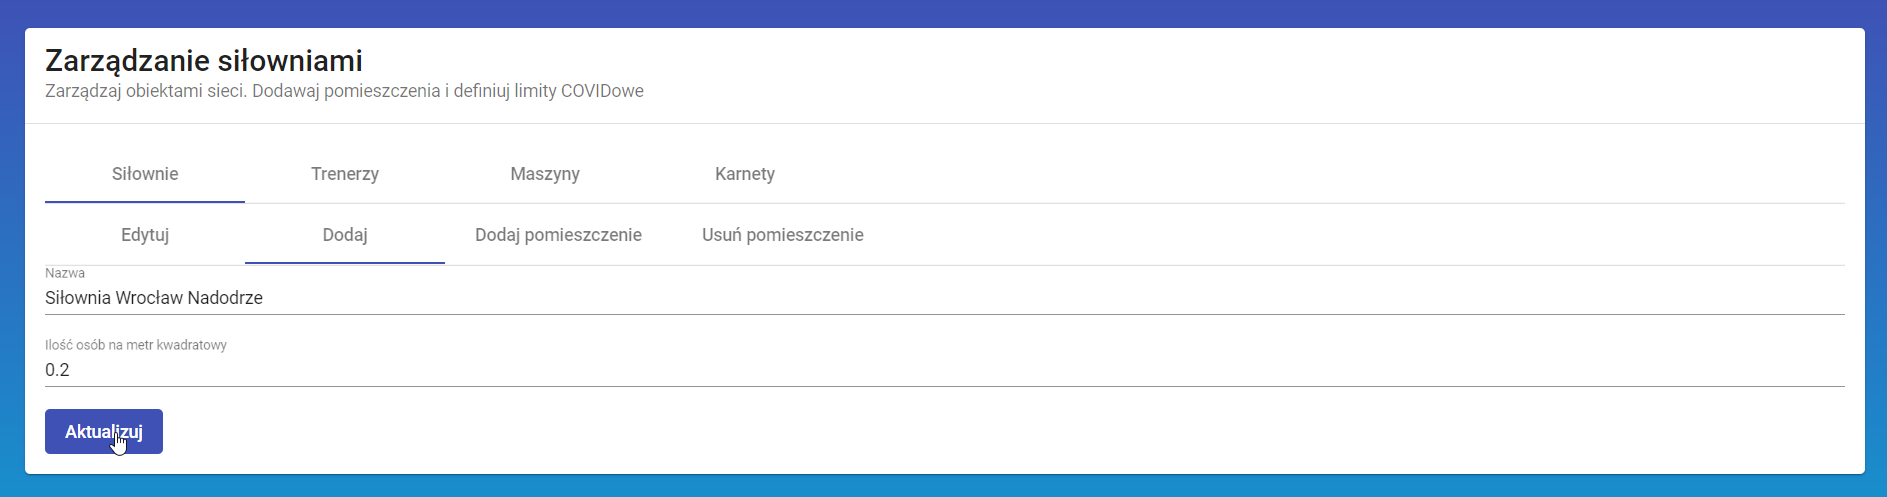
\includegraphics[width=0.75\linewidth]{../zrzuty_ekranu/dzialanie/obiekty/tworzenie}
	\caption{Formularz tworzenia obiektu siłowni}
	\label{fig:tworzenie}
\end{figure}
\FloatBarrier

\newpage
W formularzu edycji obiektów powinna wyświetlić się możliwość wybrania wcześniej utworzonej siłowni w celu aktualizacji informacji o niej. Widok ten poza edycją pozwala również na zarchiwizowanie obiektu siłowni.
\begin{figure}[h!]
	\centering
	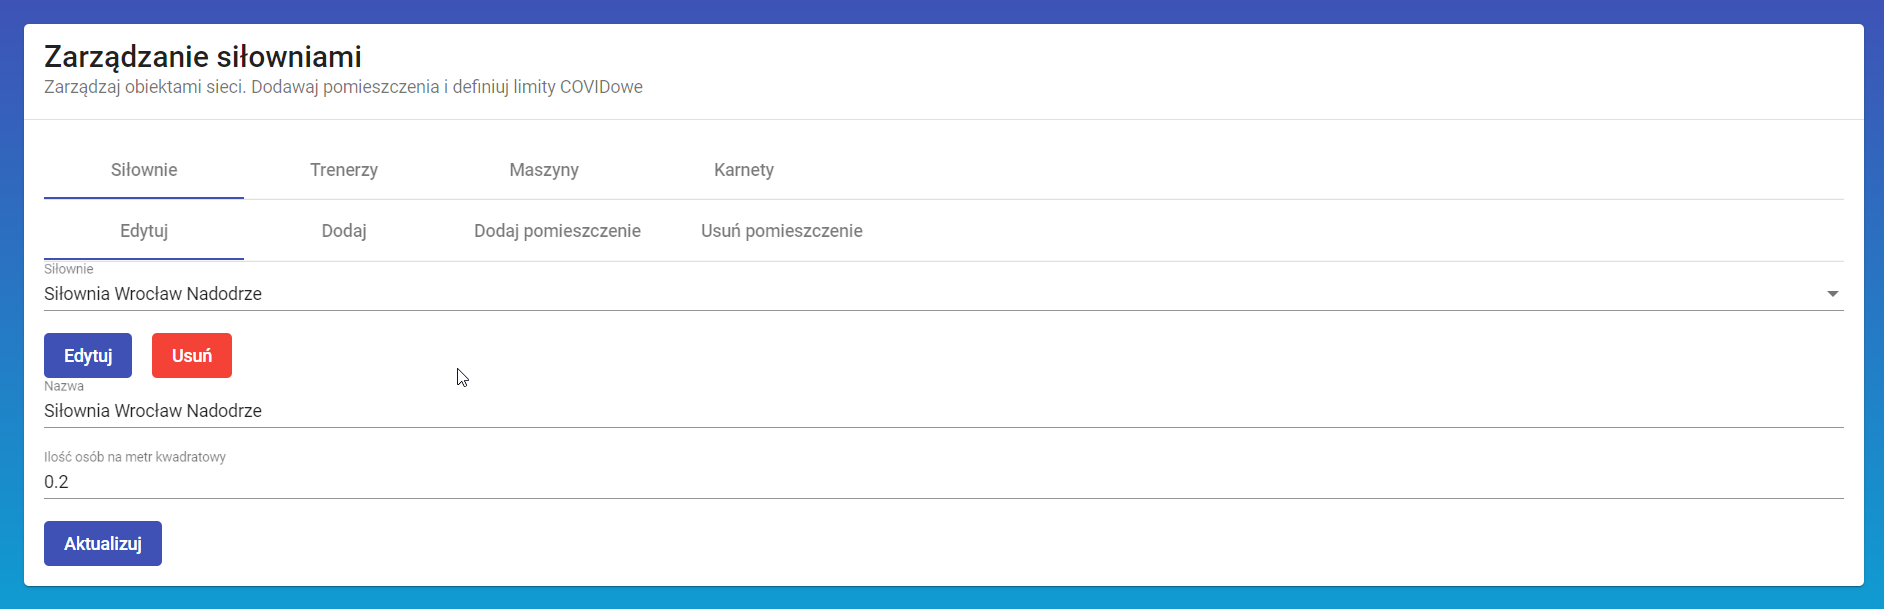
\includegraphics[width=1\linewidth]{../zrzuty_ekranu/dzialanie/obiekty/edycja}
	\caption{Formularz edycji i archiwizacji obiektów siłowni}
	\label{fig:edycja}
\end{figure}
\FloatBarrier


\subsubsection{Zarządzanie pomieszczeniami}
System udostępnia możliwość dodawania pomieszczeń do obiektów siłowni. Pomieszczenia są istotne ze względu na możliwość przypisania do nich akcesoriów do ćwiczeń oraz wyliczania maksymalnej liczby osób, która może znajdować się na siłowni. W formularzu muszą zostać podane informacje o siłowni, w której znajduje się pomieszczenie, nazwa pomieszczenia oraz jego szerokość i długość.
\begin{figure}[h!]
	\centering
	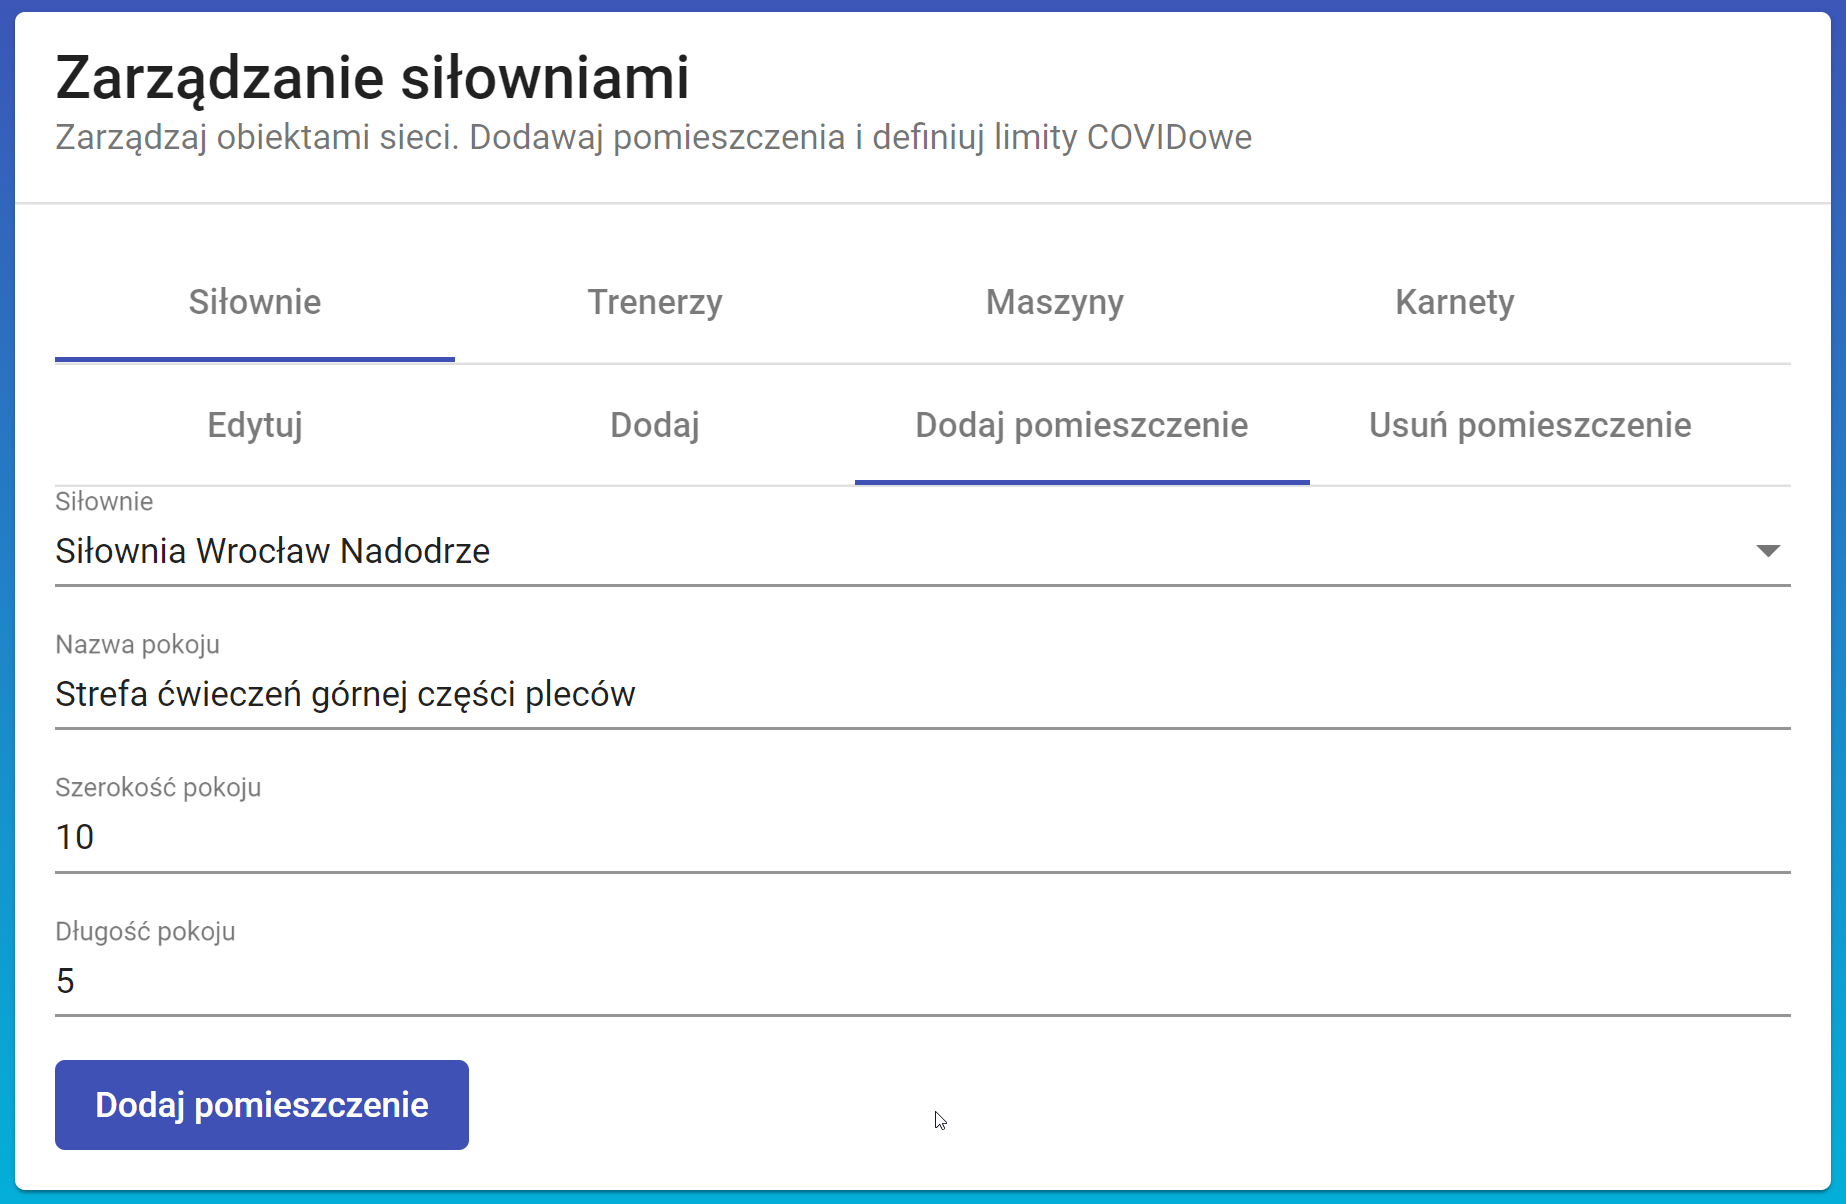
\includegraphics[width=1\linewidth]{../zrzuty_ekranu/dzialanie/pomieszczenia/dodawanie}
	\caption{Formularz dodawania pomieszczenia do obiektu siłowni}
	\label{fig:dodawanie_pomieszczenia}
\end{figure}
\FloatBarrier

Wcześniej utworzone pomieszczenie może zostać zarchiwizowane.
\begin{figure}[h!]
	\centering
	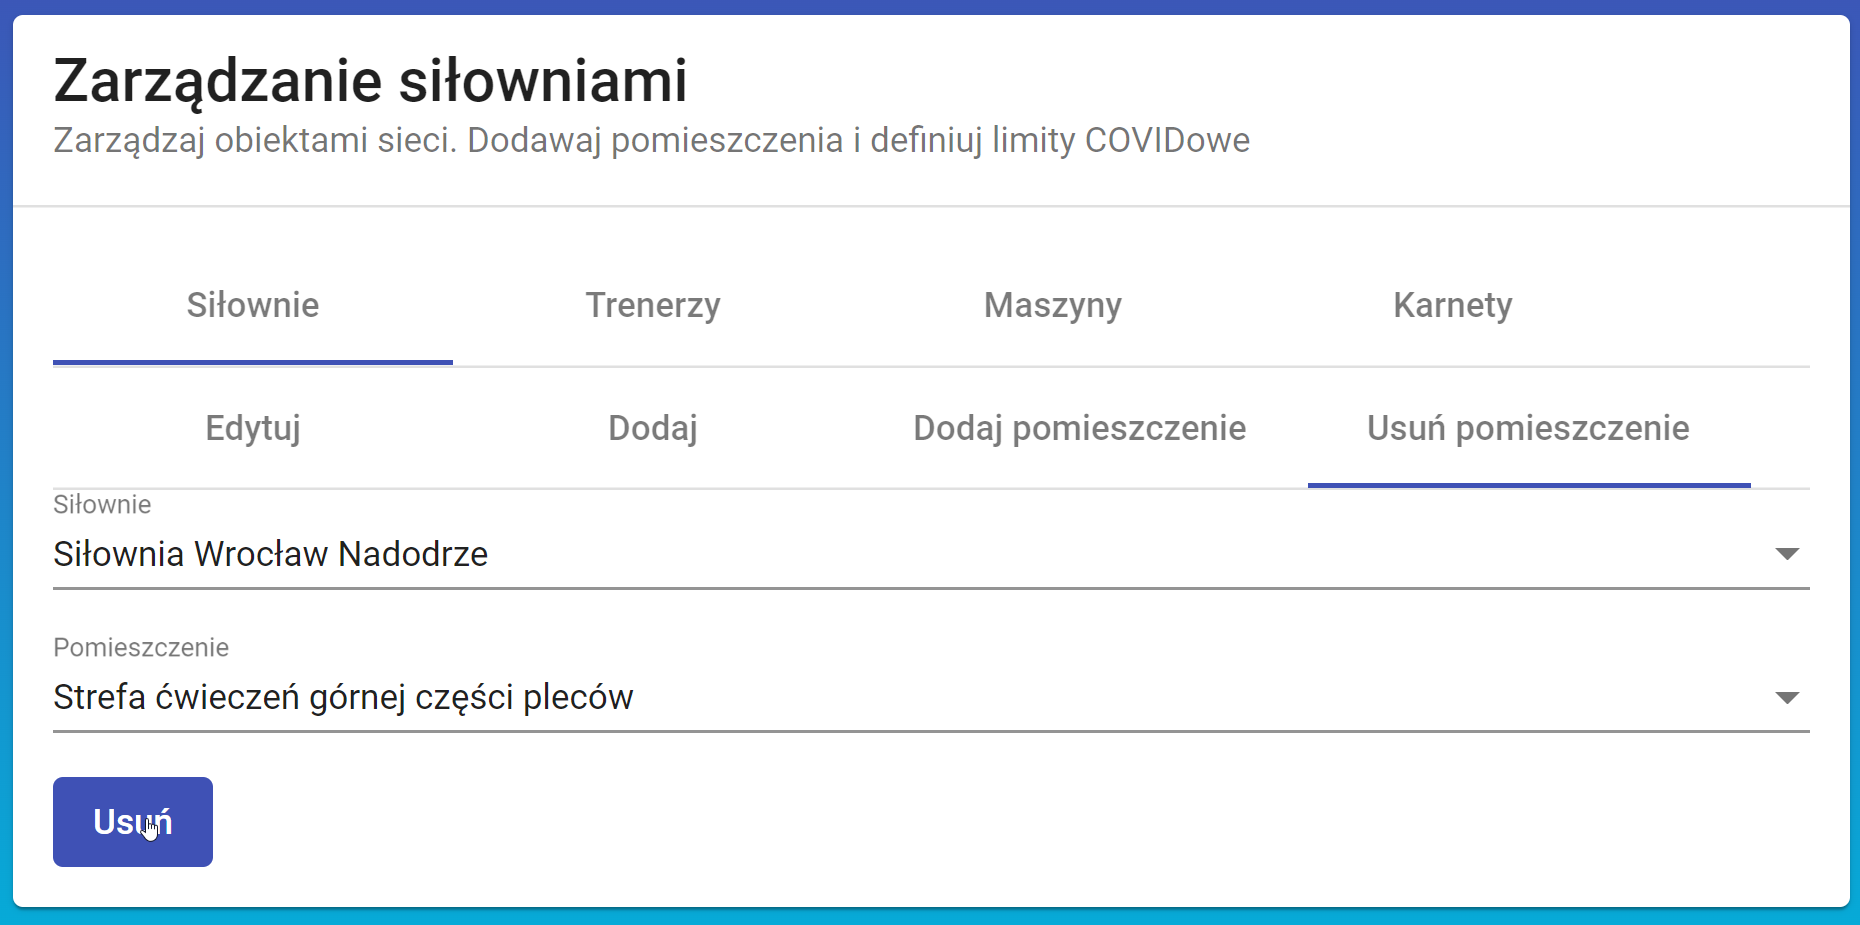
\includegraphics[width=1\linewidth]{../zrzuty_ekranu/dzialanie/pomieszczenia/usuwanie}
	\caption{Formularz archiwizacji pomieszczenia}
	\label{fig:archwizacja_pomieszczenia}
\end{figure}
\FloatBarrier


\subsubsection{Zarządzaniem sprzętem do ćwiczeń i akcesoriami}
System informatyczny powinien udostępniać możliwość stworzenia listy posiadanych akcesoriów do ćwiczeń. Dzięki takiej liście personel ma dostęp do informacji o posiadanym sprzęcie co pozwala na przeprowadzanie inwentaryzacji zasobów. Aby dodać sprzęt wymagane jest podanie informacji o kodzie producenta, nazwie, typie oraz siłowni, w której znajduje się akcesorium.
\begin{figure}[h!]
	\centering
	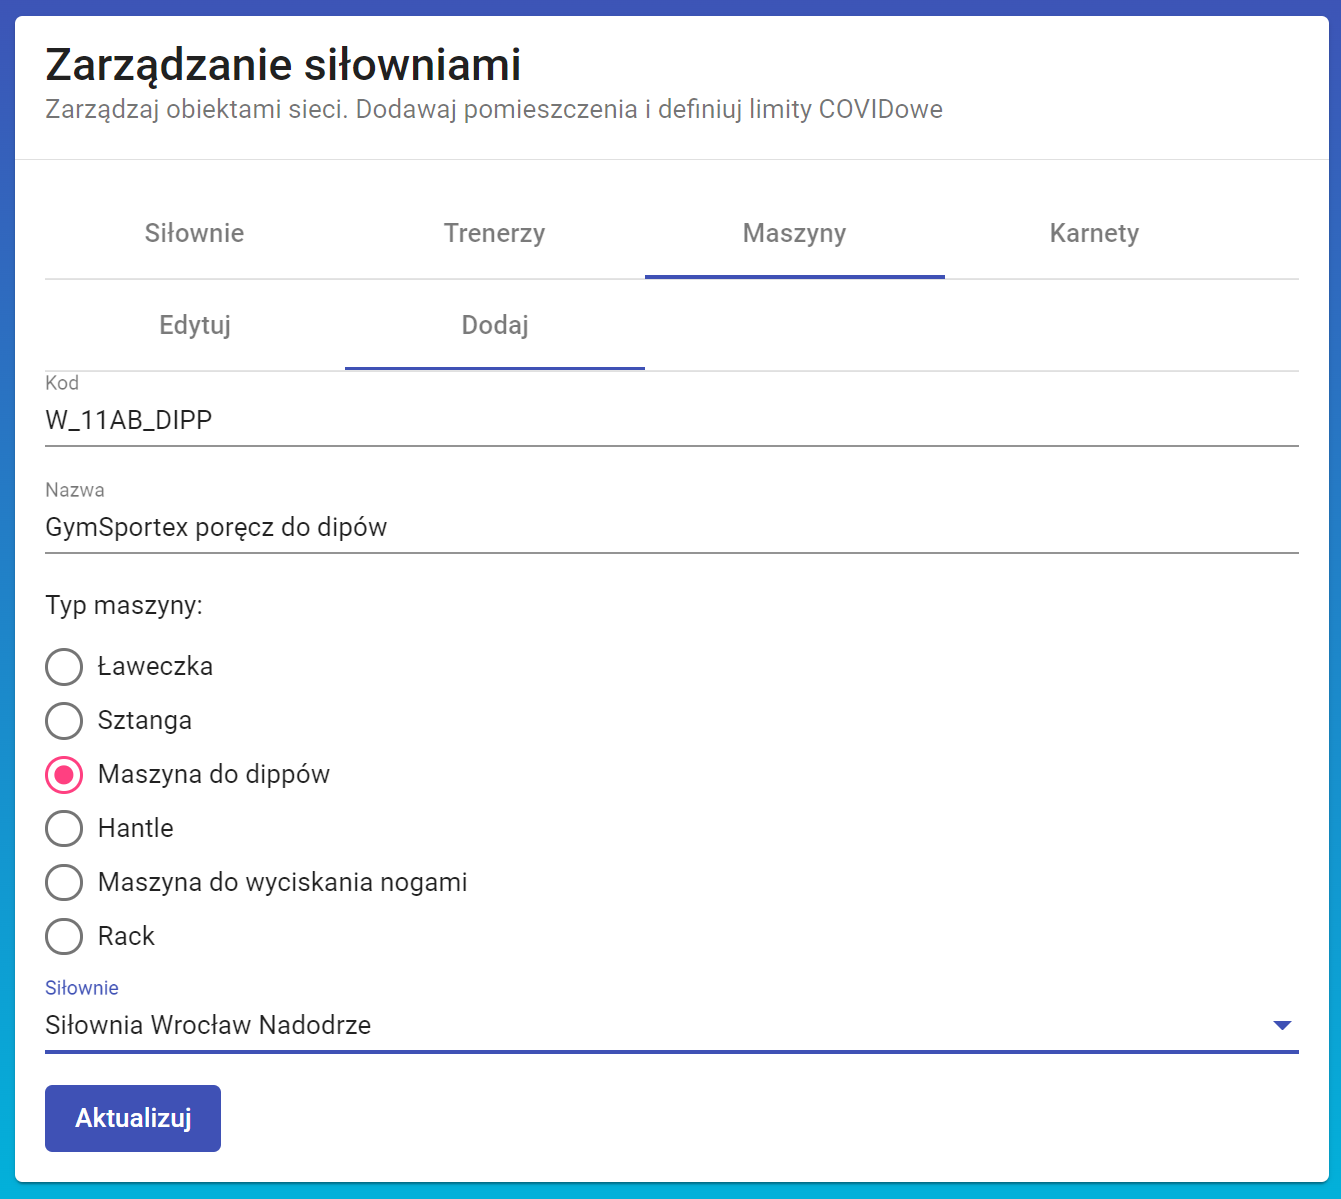
\includegraphics[width=1\linewidth]{../zrzuty_ekranu/dzialanie/akcesoria/dodawanie_akcesoriun}
	\caption{Formularz dodawania sprzętu do ćwiczeń}
	\label{fig:dodawanieakcesoriun}
\end{figure}
\FloatBarrier

Wcześniej utworzone informacje o akcesorium mogą zostać zaktualizowane lub zarchiwizowane przy pomocy formularza.
\begin{figure}[h!]
	\centering
	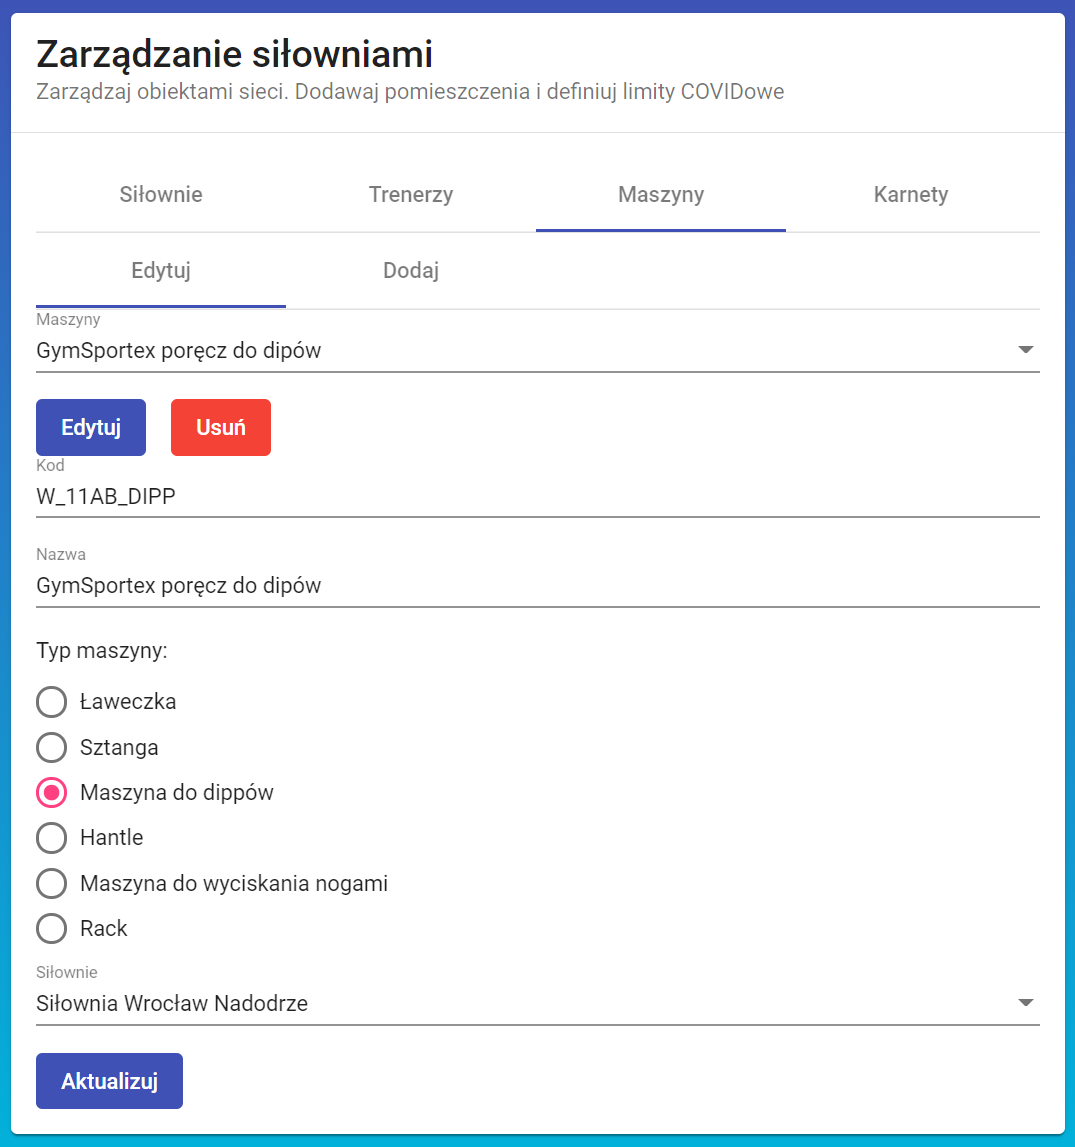
\includegraphics[width=1\linewidth]{../zrzuty_ekranu/dzialanie/akcesoria/aktualizacja_akcesorium}
	\caption{Formularz edycji i archiwizacji akcesoriów}
	\label{fig:aktualizacjaakcesorium}
\end{figure}
\FloatBarrier

\subsubsection{Zarządzanie ofertą karnetów}
Ostatnią funkcjonalnością udostępnioną przez moduł administracji jest funkcja zarządzania ofertą karnetów. System pozwala na utworzenie nowego typu karnetu, jeśli podane zostaną informacje o jego nazwie, czasie trwania w dniach oraz cenie.
\begin{figure}[h!]
	\centering
	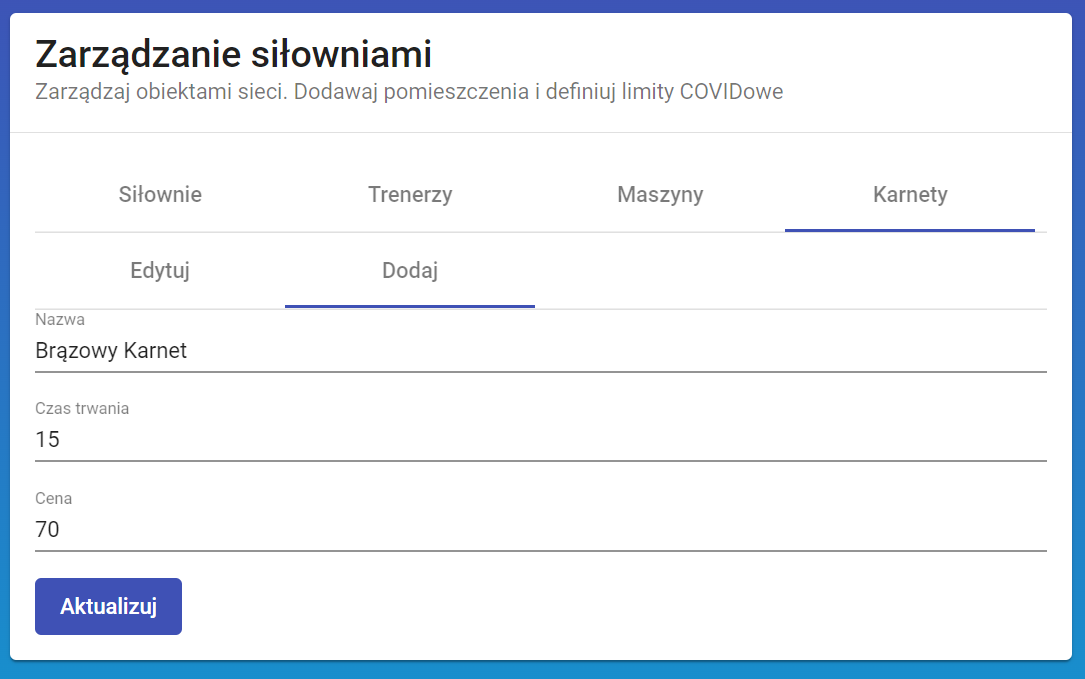
\includegraphics[width=0.8\linewidth]{../zrzuty_ekranu/dzialanie/karnety/tworzenie_karnetu}
	\caption{Formularz dodawania karnetu do oferty}
	\label{fig:tworzeniekarnetu}
\end{figure}
\FloatBarrier

Wcześniej utworzone karnety mogą zostać zaktualizowane lub zarchiwizowane.
\begin{figure}[h!]
	\centering
	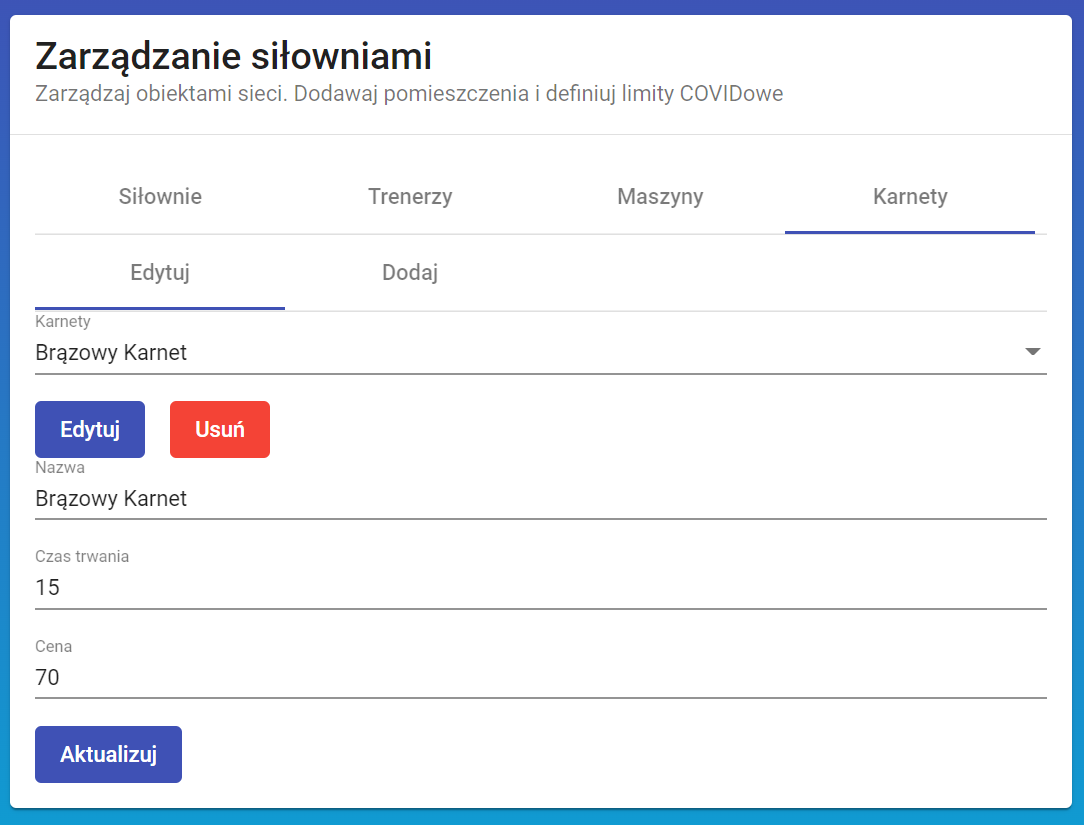
\includegraphics[width=0.8\linewidth]{../zrzuty_ekranu/dzialanie/karnety/edycja_karnetu}
	\caption{Formularz edycji i archiwizacji karnetów}
	\label{fig:edycjakarnetu}
\end{figure}
\FloatBarrier

\subsection{Wydarzenia}
Moduł wydarzeń udostępnia możliwość tworzenia, przeglądania, anulowania i zgłaszania chęci wzięcia udziału w wydarzeniu w zależności od rodzaju konta użytkownika.
\subsubsection{Tworzenie wydarzenia}
Konto trenera personalnego pozwala na tworzenie wydarzeń, w których będą mogli brać udział klienci w określonym czasie.
\begin{figure}[h!]
	\centering
	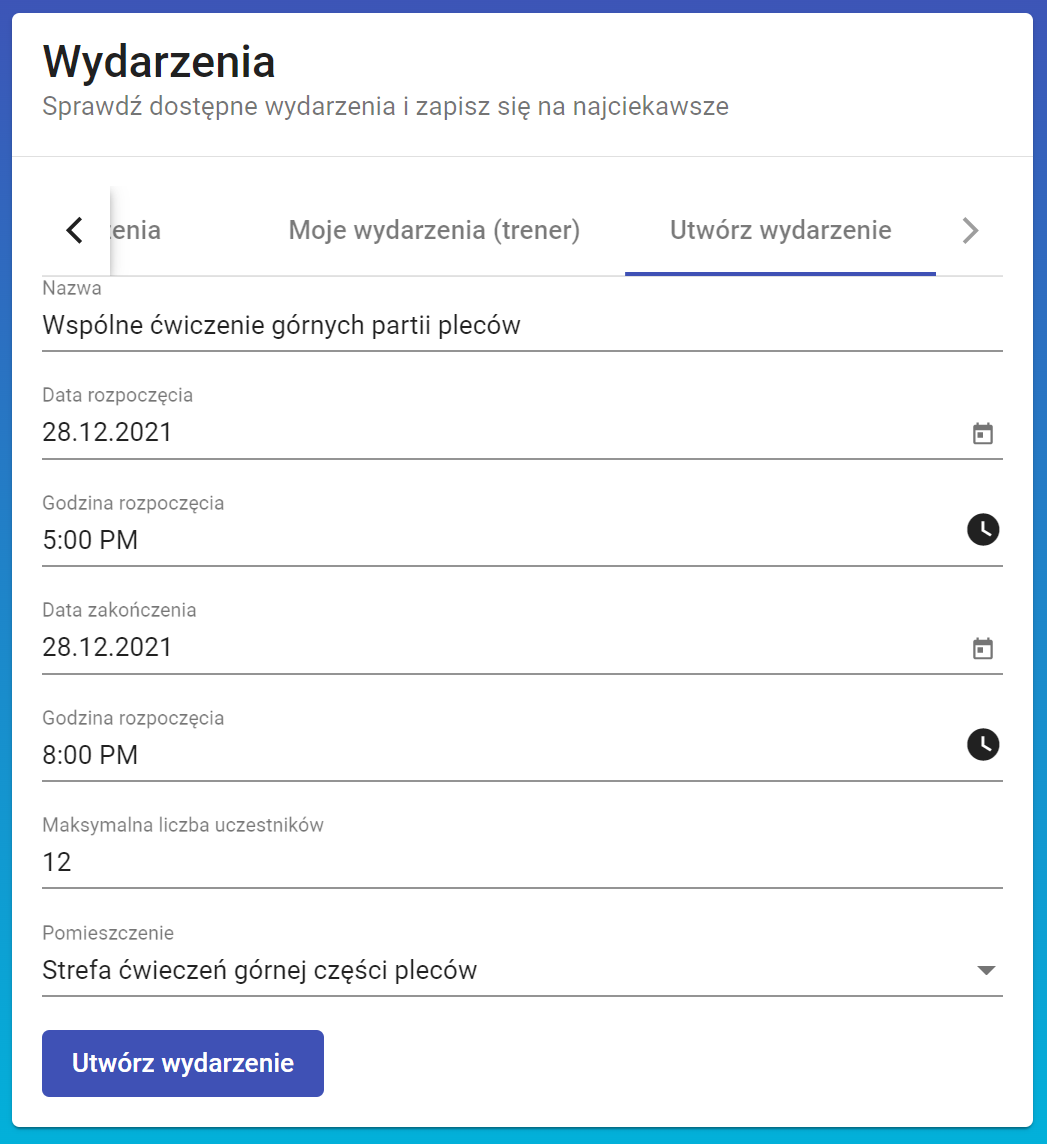
\includegraphics[width=0.8\linewidth]{../zrzuty_ekranu/dzialanie/wydarzenia/dodawanie_wydarzenia}
	\caption{Formularz tworzenia wydarzenia}
	\label{fig:dodawaniewydarzenia}
\end{figure}
\FloatBarrier

\subsubsection{Listy wydarzeń}
Klienci i trenerzy personalni mają dostęp do listy wszystkich wydarzeń. Z poziomu tej listy użytkownicy mogą przejść do poglądu wydarzenia, gdzie znajdują się dodatkowe opcje zarządzania wydarzeniem.
\begin{figure}[h!]
	\centering
	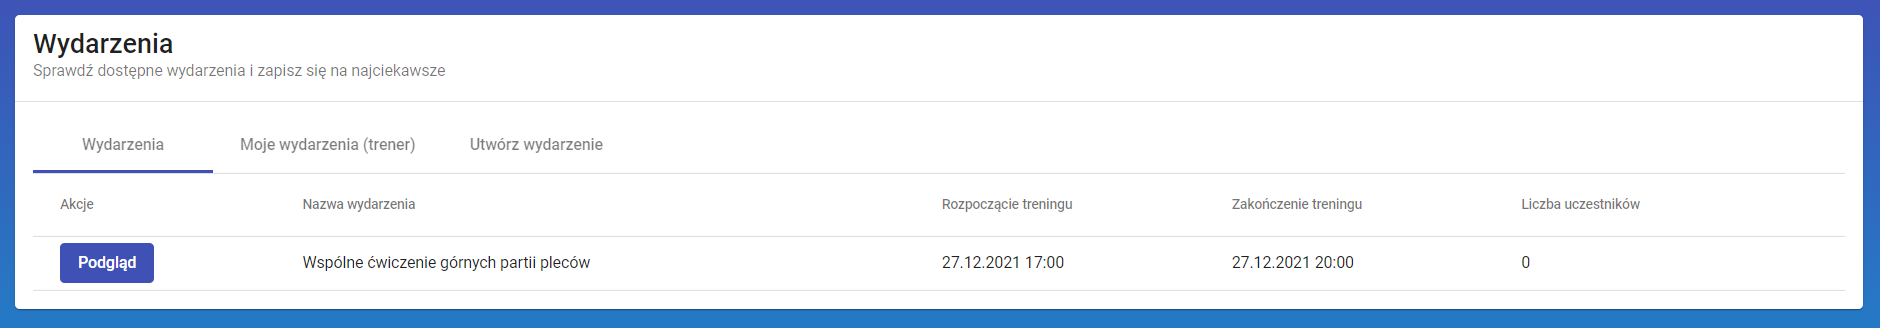
\includegraphics[width=1\linewidth]{../zrzuty_ekranu/dzialanie/wydarzenia/wszystkie_wydarzenia}
	\caption{Lista wszystkich wydarzeń}
	\label{fig:wszystkiewydarzenia}
\end{figure}
\FloatBarrier
Trenerzy personalni mają dodatkowo możliwość wyświetlenia listy wydarzeń, które sami utworzyli.
\begin{figure}[h!]
	\centering
	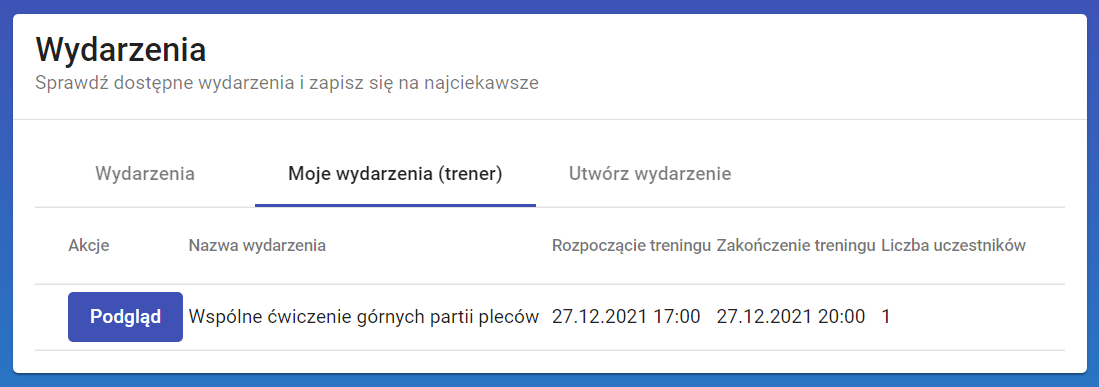
\includegraphics[width=1\linewidth]{../zrzuty_ekranu/dzialanie/wydarzenia/trener_lista_wydarzen}
	\caption{Lista utworzony wydarzeń przez trenera personalnego}
	\label{fig:trenerlistawydarzen}
\end{figure}
\FloatBarrier
\newpage
Klienci natomiast mają możliwość wyświetlenia wydarzeń, w których zgłosili chęć wzięcia udziału.
\begin{figure}[h!]
	\centering
	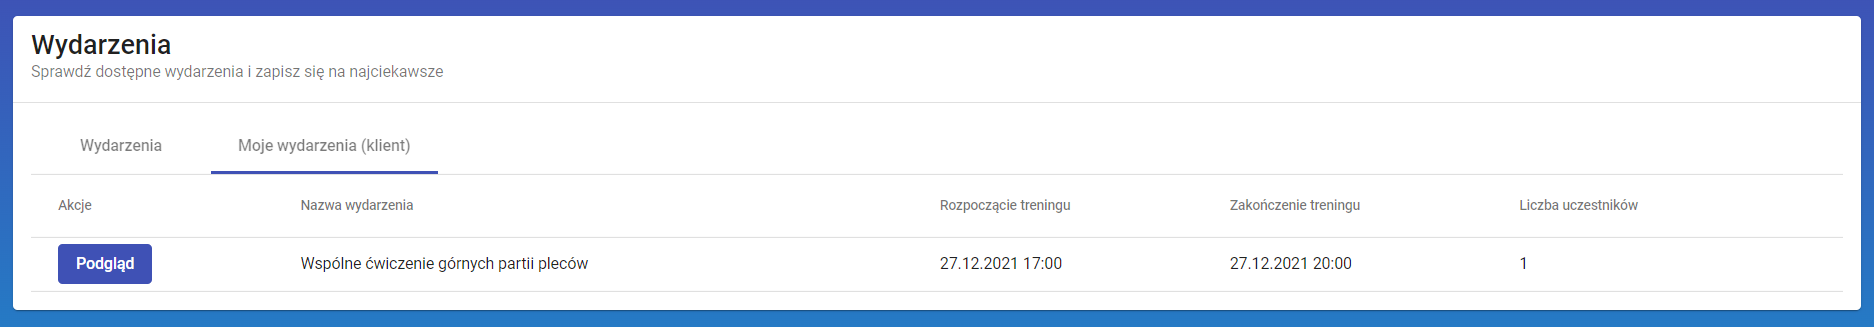
\includegraphics[width=0.9\linewidth]{../zrzuty_ekranu/dzialanie/wydarzenia/klient_lista_wydarzen}
	\caption{Lista wydarzeń klienta}
	\label{fig:klientlistawydarzen}
\end{figure}
\FloatBarrier

\subsubsection{Podgląd wydarzeń}
Systemu udostępnia widok podglądu wydarzenia. Użytkownicy mogą przeglądać wszystkie wydarzenia, ale dostępne opcje są zależne od roli jaką pełnią. Trener personalny w podglądzie wydarzenia zobaczy opcję anulowania wydarzenia.
\begin{figure}[h!]
	\centering
	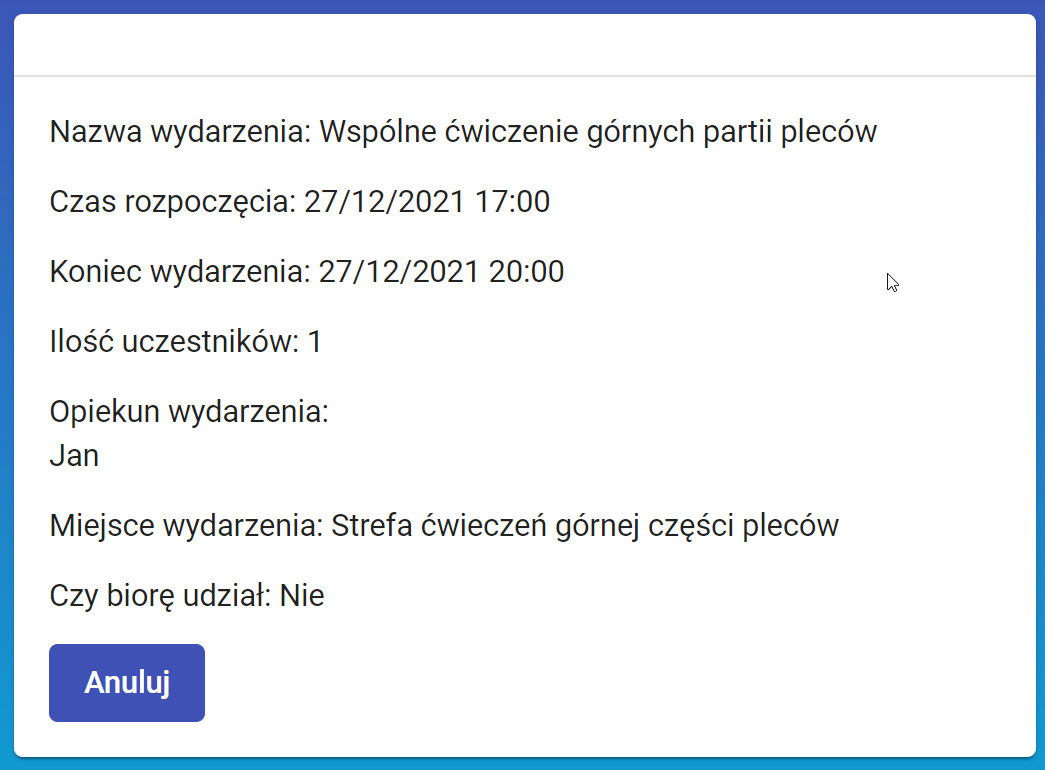
\includegraphics[width=0.7\linewidth]{../zrzuty_ekranu/dzialanie/wydarzenia/trener_podlad_wydarzenie}
	\caption{Podgląd wydarzenia jako trener personalny}
	\label{fig:trenerpodladwydarzenie}
\end{figure}
\FloatBarrier
Klient na tym samym widoku zobaczy opcję zgłoszenia chęci udziału w wydarzeniu lub zrezygnowania z niego.
\begin{figure}[h!]
	\centering
	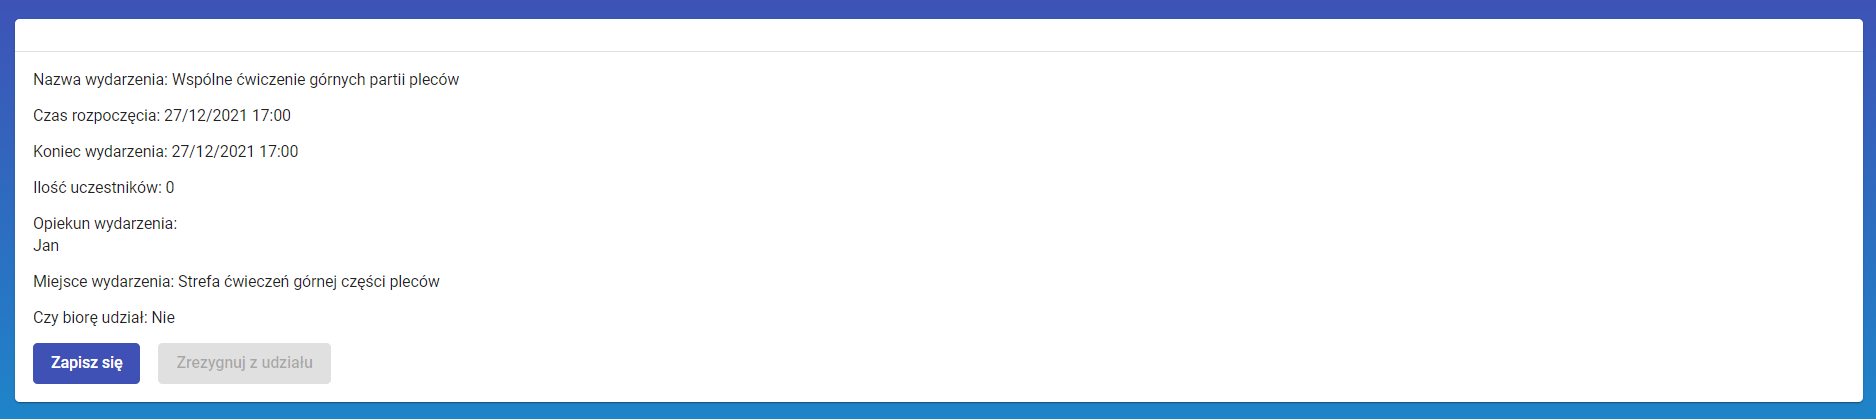
\includegraphics[width=1\linewidth]{../zrzuty_ekranu/dzialanie/wydarzenia/klient_podlad_wydarzenia}
	\caption{Pogląd wydarzenia jako klient}
	\label{fig:klientpodladwydarzenia}
\end{figure}
\FloatBarrier
\subsection{Treningi indywidualne}
Kolejnym modułem w systemie jest moduł treningów indywidualnych. Moduł ten pozwala na organizowanie treningów, w których brać będzie udział klient pod nadzorem trenera personalnego. Pozwala to na utworzenie oferty dostosowanej do klientów, którzy chcą ćwiczyć pod okiem specjalistów.
\FloatBarrier

\newpage
\subsubsection{Tworzenie treningów indywidualnych}
Trener personalny posiada możliwość utworzenia treningu. Aby dodać trening, użytkownik z rolą trenera musi wskazać w formularzu, gdzie odbędzie się trening oraz w jakim terminie.
\begin{figure}[h!]
	\centering
	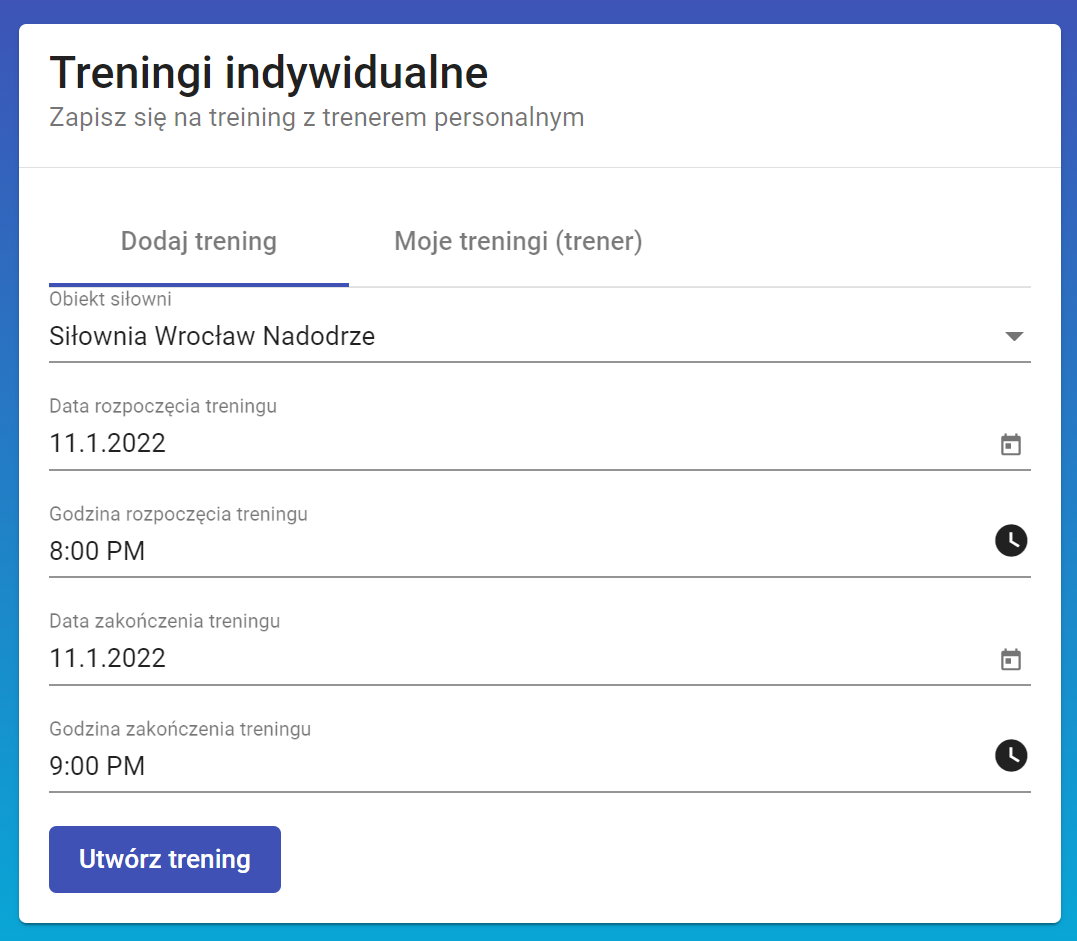
\includegraphics[width=1\linewidth]{../zrzuty_ekranu/dzialanie/treningi/dodawanie_treningu}
	\caption{Formularz dodawania treningu}
	\label{fig:dodawanietreningu}
\end{figure}
\FloatBarrier

\subsubsection{Listy treningów indywidualnych}
System pozwala klientom na pogląd listy dostępnych treningów. Treningi w~statusie \textit{Open} oznaczają treningi, w których żaden użytkownik nie zgłosił chęci wzięcia udziału.
\begin{figure}[h!]
	\centering
	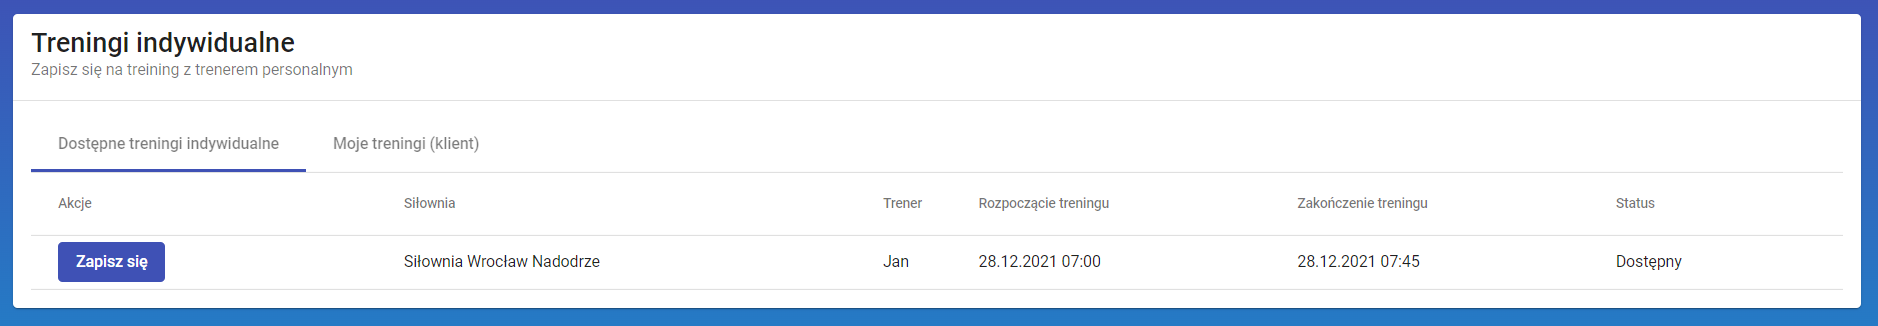
\includegraphics[width=1\linewidth]{../zrzuty_ekranu/dzialanie/treningi/klient_dostepne_treningi}
	\caption{Lista dostępnych treningów indywidualnych}
	\label{fig:klientdostepnetreningi}
\end{figure}
\FloatBarrier
Z perspektywy klienta dostępna jest również lista treningów, na które się zapisał. Dzięki tej liście klient będzie mógł sprawdzić na jakich treningach był oraz jakie go jeszcze czekają.
\begin{figure}[h!]
	\centering
	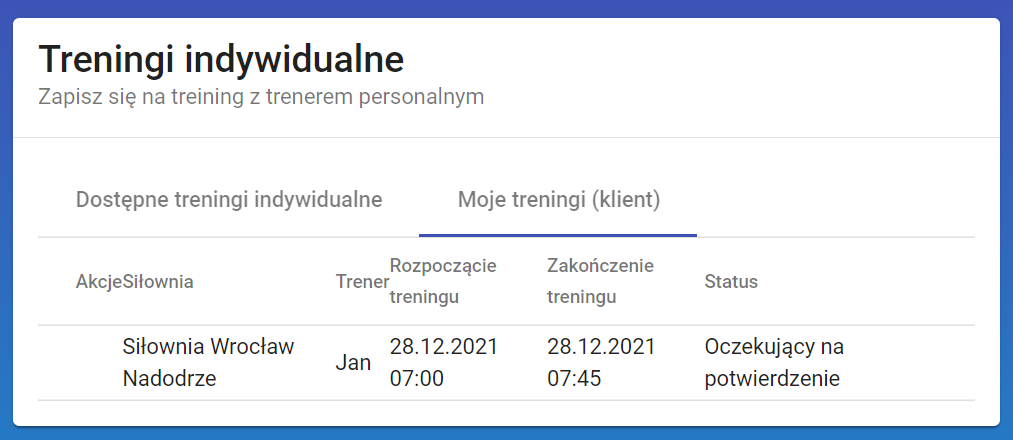
\includegraphics[width=1\linewidth]{../zrzuty_ekranu/dzialanie/treningi/klient_lista_treningow}
	\caption{Lista treningów, na które zapisał się klient}
	\label{fig:klientlistatreningow}
\end{figure}
\FloatBarrier
Trener personalny natomiast posiada możliwość poglądu utworzonych przez siebie wydarzeń. Lista pozwala na odwołanie treningu lub potwierdzenie go.\\To jakie opcje są dostępne jest zależne od statusu w jakim znajduje się dany trening.
\begin{figure}[h!]
	\centering
	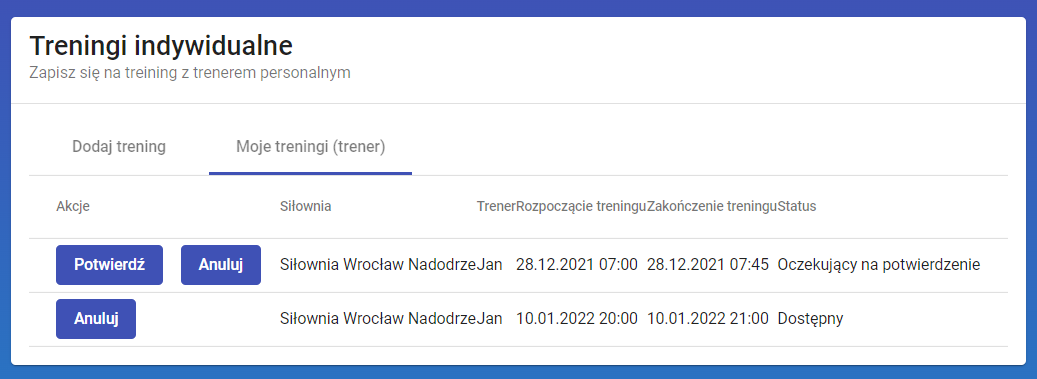
\includegraphics[width=0.9\linewidth]{../zrzuty_ekranu/dzialanie/treningi/trener_lista_treningow}
	\caption{Lista utworzonych treningów przez trenera}
	\label{fig:trenerlistatreningow}
\end{figure}
\FloatBarrier

\subsection{Karnety}
System posiada moduł karnetów, gdzie klient może sprawdzić ważność karnetu, dostępną ofertę, zakupić lub przedłużyć karnet.
\begin{figure}[h!]
	\centering
	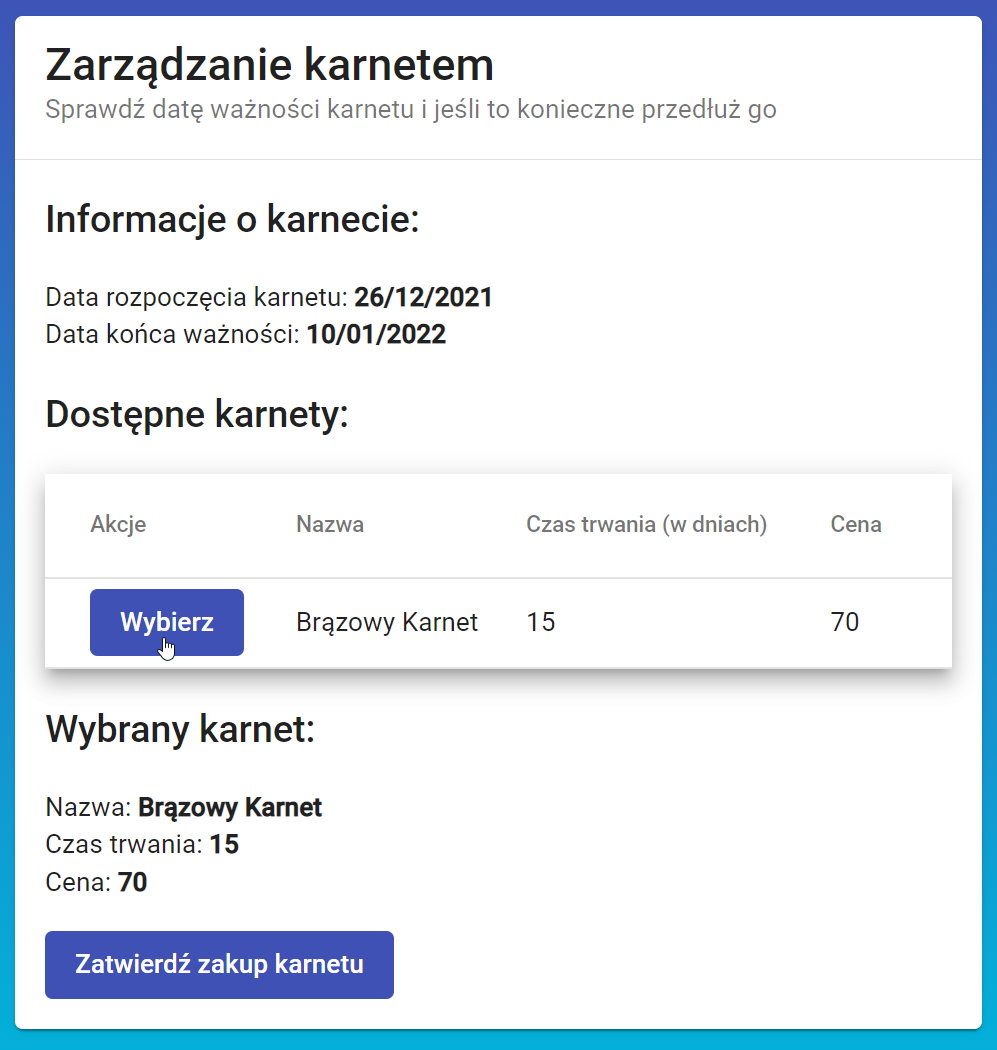
\includegraphics[width=0.5\linewidth]{../zrzuty_ekranu/dzialanie/karnety/lista_karnetow}
	\caption{Oferta karnetów oraz informacje o posiadanym karnecie}
	\label{fig:listakarnetow}
\end{figure}
\FloatBarrier

\subsection{Tryb bramek}
Istotnym z punktu widzenia pandemicznych obostrzeń jest moduł bramek. System udostępnia tryb bramek, które pozwala na podłączenie aplikacji do bramek i~wyświetlaczy w celu kontroli liczby osób znajdujących aktualnie na siłowni.
\subsubsection{Bramka wejściowa}
Głównym zadaniem bramki wejściowej jest kontrolowanie ważności posiadanego karnetu oraz kontroli czy na siłowni nie znajduje się zbyt duża liczba osób w~stosunku do obowiązujących obostrzeń. Aby wejść na siłownie klient musi podać lub zeskanować za pomocą skanera swój kod identyfikacyjny. Formularz powinien w tym momencie wyświetlić informację o tym czy istnieje możliwość wejścia na siłownie. To czy można wejść na siłownię zależy od liczby osób, która znajduje się na siłowni oraz ważności karnetu klienta.
\begin{figure}[h!]
	\centering
	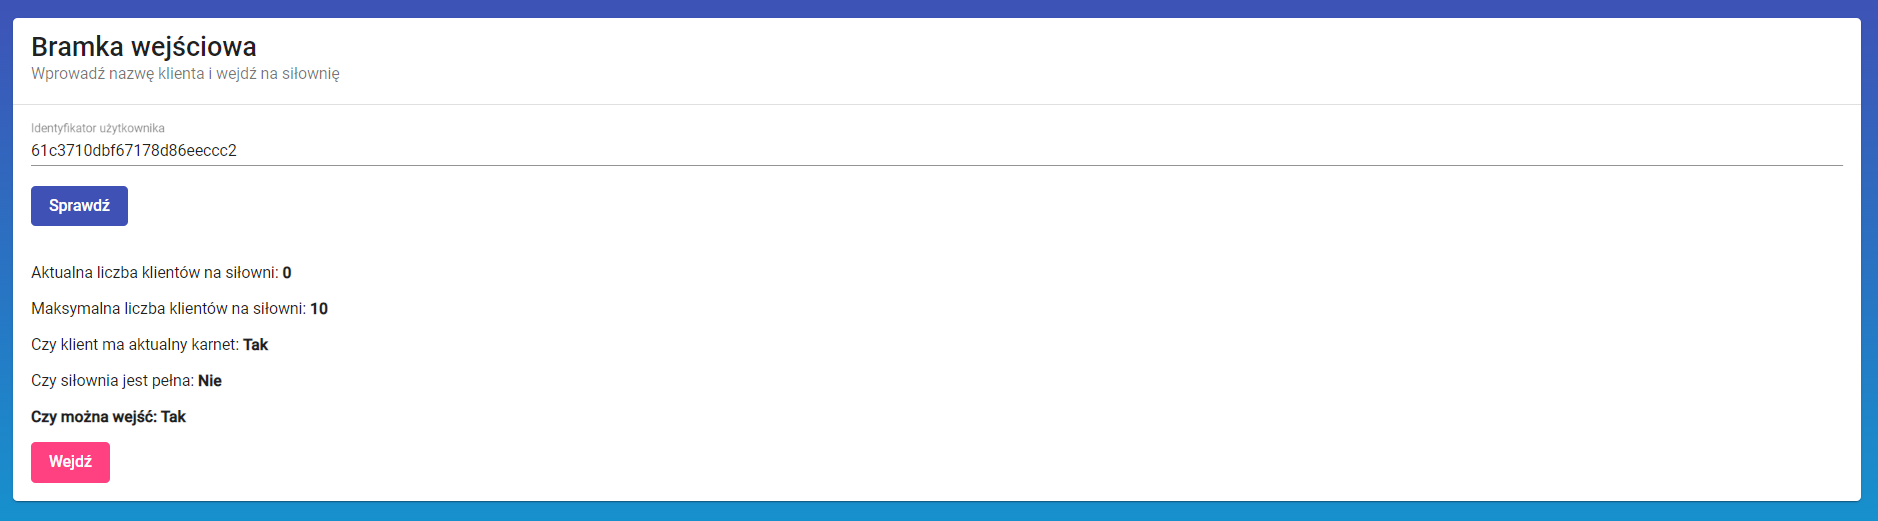
\includegraphics[width=0.8\linewidth]{../zrzuty_ekranu/dzialanie/bramki/bramka_wejsciowa}
	\caption{Widok wyświetlany na wyświetlaczu bramki wejściowej}
	\label{fig:bramkawejsciowa}
\end{figure}
\FloatBarrier

\subsubsection{Bramka wyjściowa}
Zadaniem bramki wyjściowej jest usuwanie z listy klientów osób, które już nie korzystają z usług danego obiektu siłowni.
\begin{figure}[h!]
	\centering
	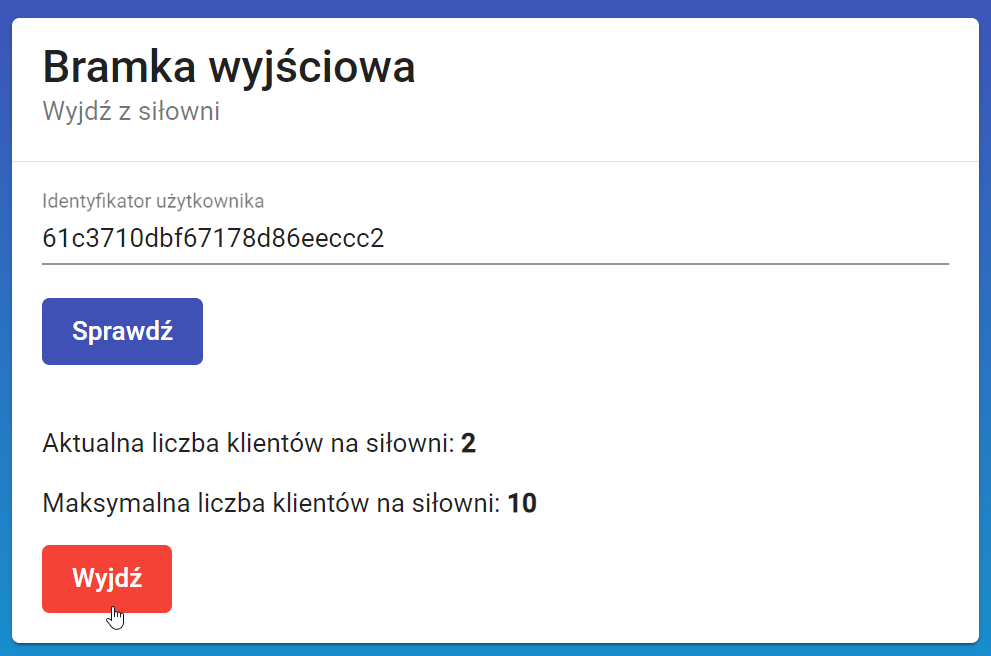
\includegraphics[width=1\linewidth]{../zrzuty_ekranu/dzialanie/bramki/bramka_wyjsciowa}
	\caption{Widok wyświetlany na wyświetlaczu bramki wyjściowej}
	\label{fig:bramkawyjsciowa}
\end{figure}
\FloatBarrier

\chapter{Specyfikacja wewnętrzna}
\label{chap:internal}
Rozdział rozpoczyna się od opisania architektury systemu z podziałem na warstwy z uwzględnieniem komunikacji pomiędzy nimi. W dalszej części rozdziału znajduje się przedstawienie organizacji bazy danych. Następnie w rozdziale przedstawiono przegląd najważniejszych klas i algorytmów. Rozdział zakończony jest opisem zastosowanych wzorców projektowych.

\section{Architektura systemu}
System został podzielony na dwie główne warstwy. Architektura została zaprezentowana na rysunku \ref{fig:architektura}.
\begin{figure}[htbp]
	\centering
	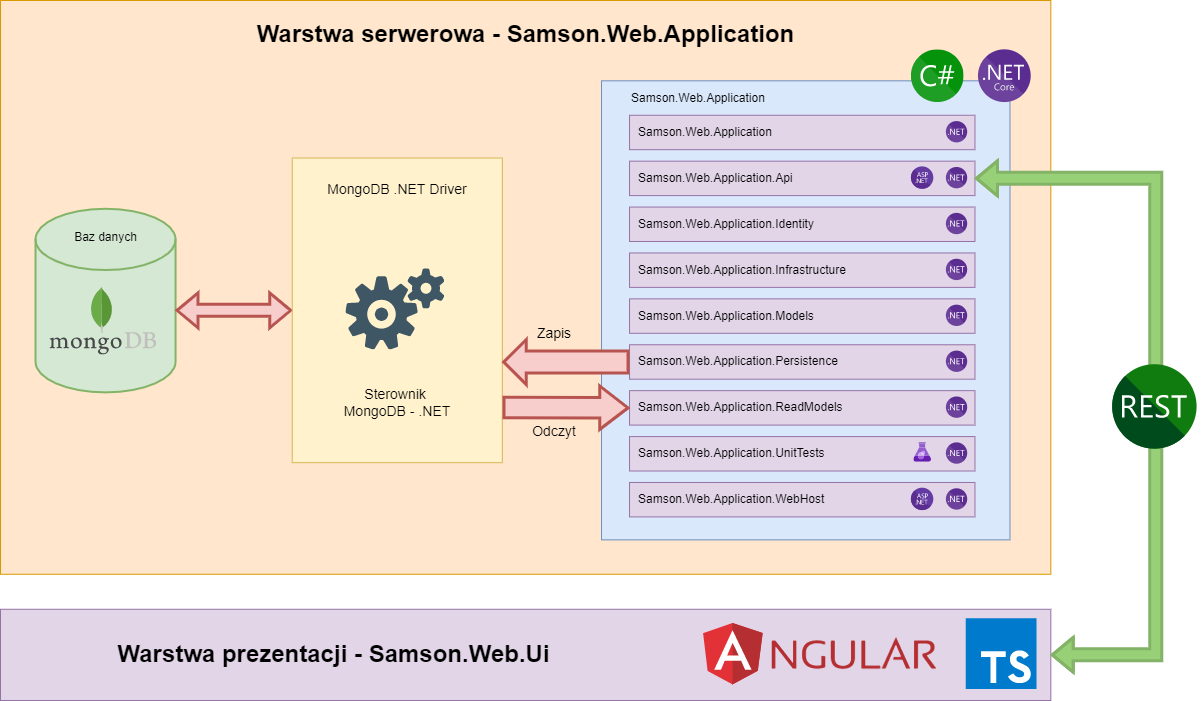
\includegraphics[width=1\linewidth]{../diagramy/architektura}
	\caption{Architektura systemu}
	\label{fig:architektura}
\end{figure}

\subsubsection{Warstwa serwerowa}
Warstwa serwerowa to część aplikacji znajdująca się na serwerze. Jej głównym zadaniem jest obsługiwanie żądań wysyłanych przez część kliencką systemu. Warstwa serwerowa składa się z głównego projektu \textit{Samson.Web.Application}, w którego skład wchodzą projekty platformy .NET:
\begin{itemize}
	\item \textit{Samson.Web.Application} - projekt w skład którego wchodzą serwisy aplikacyjne realizujące logikę biznesową. Ważnymi składowymi projektu są klasy obsługi komend (ang. \ang{command handler}), których zadaniem jest aktualizacja danych oraz klasy obsługi zapytań (ang. \ang{query handler}), które odpowiadają za odczyt danych z bazy.
	\item \textit{Samson.Web.Application.Api} - projekt, który przy pomocy kontrolerów (ang. \ang{controllers}) obsługuje otrzymane żądania z warstwy klienckiej. Metoda klasy kontrolera tworzy komendę (ang. \ang{command}) lub zapytanie (ang. \ang{query}), które jest następnie przekazywane do mediatora (ang. \ang{mediator}). Mediator rozdziela je do odpowiedniej klasy obsługi komendy lub klasy obsługi zapytań. Takie podejście pozwala na stworzenie skalowalnej architektury podatnej na zmiany. Dzięki takiemu podejściu klasy kontrolerów nie muszą wstrzykiwać zależności w postaci serwisów aplikacyjny lub klas repozytorium (ang. \ang{repository}).
	\item \textit{Samson.Web.Application.Identity} - to projekt odpowiedzialny za tworzenie żetonów JWT oraz sprawdzanie ich poprawności. \textit{Samson.Web.Application.Identity} pełni kluczową rolę w ochronie systemu przed nieautoryzowanym dostępem.
	\item \textit{Samson.Web.Application.Infrastructure} - projekt w skład, którego wchodzą atrybuty, oprogramowanie pośrednie (ang. \ang{middleware}) oraz klasy wykorzystywane w pozostały projektach warstwy serwerowej. Projekt zawiera także klasy globalnej obsługi błędów (ang. \ang{global error handler}), których zadaniem jest przechwytywanie wyjątków (ang. \ang{exception}), które nie zostały wcześniej obsłużone.
	\item \textit{Samson.Web.Application.Models} - projekt zawierający klasy modeli, obiekty transferu danych (ang. \ang{data transfer object}), struktury danych oraz wyliczenia (ang. \ang{enum}).
	\item \textit{Samson.Web.Application.Persistence} - projekt pełniący kluczową rolę, jeśli chodzi o zapis danych. Projekt zawiera klasy encji (ang. \ang{entity}) oraz klasy repozytoriów. Klasy repozytoriów tworzą warstwę odpowiedzialną za aktualizację danych przy pomocy sterownika \textit{MongoDB .NET Driver}.
	\item \textit{Samson.Web.Application.ReadModels} - w przeciwieństwie do poprzedniego projektu, w skład \textit{Samson.Web.Application.ReadModels} wchodzą klasy odpowiedzialne za odczyt danych z bazy. Zadanie to jest realizowana przy wykorzystaniu klas odczytu modeli (ang. \ang{read model}), w których znajduje się kod realizujący zapytania do bazy przy pomocy wstawek \textit{JavaScript} lub składni \textit{LINQ}.
	\item \textit{Samson.Web.Application.UnitTests} - projekt zawierający kod testów jednostkowych
	\item \textit{Samson.Web.Application.WebHost} - projekt, który jest punktem początkowym aplikacji. W projekcie można znaleźć pliki konfiguracji z rozszerzeniem \textit{JSON}.
\end{itemize}
Istotną częścią warstwy serwerowej jest baza danych, która odpowiada za przechowywanie danych w sposób uporządkowany i trwały. Projekt główny realizuje komunikację z bazą danych przy pomocy sterownika, który pozwala na zintegrowanie technologii \textit{.NET} i bazy \textit{MongoDB}.

\subsubsection{Warstwa prezentacji}
Warstwa prezentacji wysyła żądania do warstwy serwerowej przy pomocy metod \textit{HTTP} i interfejsu \textit{REST API}, który jest punktem łączącym obie warstwy. Podstawowym zadaniem, które realizuje ta warstwa jest graficzna prezentacja funkcjonalności w celu uproszczenia korzystania z systemu.

\section{Organizacja bazy danych}
Baza danych \textit{MongoDB} jest dokumentową, niereleacyjną bazą danych \textit{NoSQL}, więc nie posiada typowej struktury bazy \textit{SQL}. W przeciwieństwie do baz relacyjnych w bazie \textit{MongoDB} często stosuje się denormalizacje struktury w celu poprawienia wydajności odczytu danych. Wadą tego rozwiązania jest potrzeba ręcznego aktualizowania powielonych dokumentów oraz mniejsza wydajność zapisu.

Zaprezentowany schemat bazy prezentuje kolekcje dokumentów, jakie zawiera baza. Na schemacie uwzględnione zostały relacje, które utworzono przy wykorzystaniu referencji. Takie podejście pozwala na wprowadzenie normalizacji danych i~uniknięcie powielania dokumentów \cite{bib:mongoRelations}.

\begin{figure}[htbp]
	\centering
	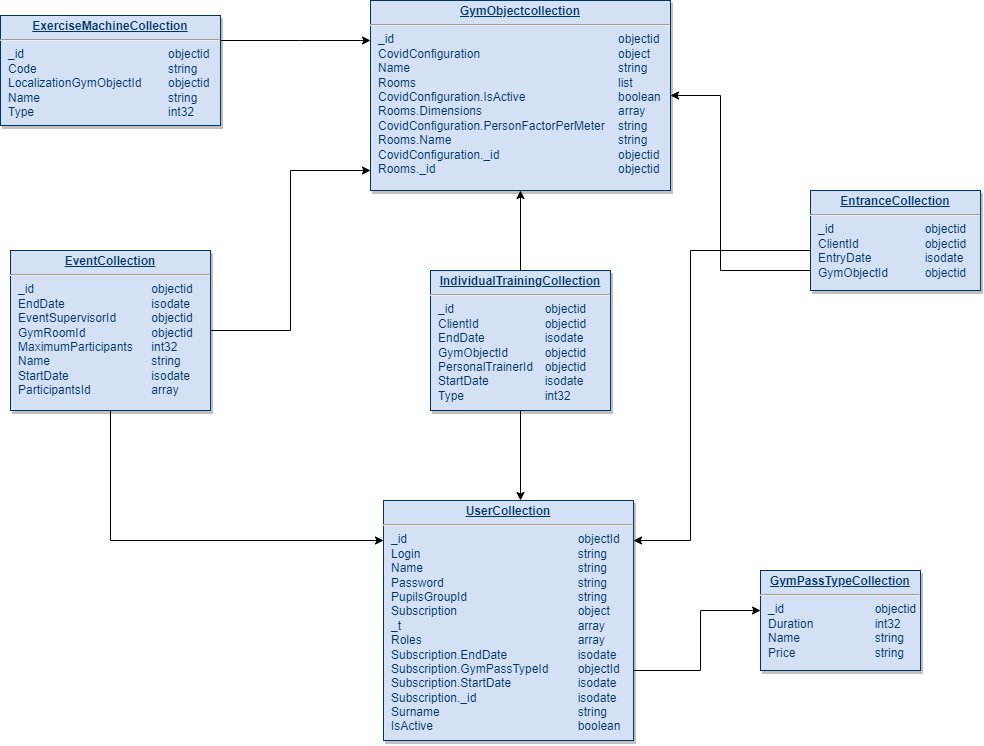
\includegraphics[width=1\linewidth]{../diagramy/schemat_bazy}
	\caption{Poglądowy schemat bazy danych}
	\label{fig:schematbazy}
\end{figure}

Poszczególne kolekcje zostały podzielone według funkcjonalności, którym odpowiadają:
\begin{itemize}
	\item \textit{ExerciseMachineCollection} - kolekcja zawierająca informacje o akcesoriach do ćwiczeń. Dokumenty w kolekcji zawierają referencję do \textit{GymObjectCollection}. Referencja została zrealizowana przy pomocy klucza \textit{LocalizationGymObjectId}, który pozwala na określenie gdzie znajduje się dany przyrząd do ćwiczeń.
	\item \textit{GymObjectCollection} - kolekcja przechowująca informacje o obiektach i pomieszczeniach siłowni.
	\item \textit{EventCollection} - zawiera informację o wydarzeniach organizowanych przez sieć. Kolekcja ta posiada referencje do kolekcji \textit{GymObjectCollection} i \textit{UserCollection}.
	\item \textit{IndividualTraniningCollection} - kolekcja odpowiedzialna za przechowywanie informacji o treningach indywidualnych. W celu określenia miejsca treningu posiada referencję do kolekcji \textit{GymObjectCollection}. Organizator i klienci biorący udział w wydarzeniu są odnajdywani w bazie przy użyciu referencji do \textit{UserCollection}.
	\item \textit{EntranceCollection} - kolekcja zawierająca informacje o klientach, którzy znajdują się wewnątrz siłowni.
	\item \textit{UserCollection} - kolekcja przechowująca informacje o klientach i trenerach personalnych.
	\item \textit{GymPassTypeCollection} - kolekcja w ramach, której znajdują się dokumenty opisujące rodzaje karnetów, które są oferowane przez sieć.
\end{itemize}

\section{Przegląd najważniejszych klas}
W trakcie pracy nad systemem zaistniała potrzeba stworzenia klasy pozwalającej na modyfikacje danych w bazie. Głównym założeniem było utworzenie klasy, która będzie wykorzystywać wzorzec repozytorium oraz metodę szablonową. Wzorzec repozytorium miał pomóc w stworzeniu klasy, której głównym zadaniem będzie realizowanie operacji \textit{CRUD}, natomiast wykorzystanie wzorca metody szablonowej miało pomóc w stworzeniu ogólnego algorytmu, który będzie uszczegółowiony w klasach pochodnych. Według tych zasad powstała abstrakcyjna klasa \textit{MongoRepository} reprezentująca ogólne algorytmy wykorzystywane do operacji \textit{CRUD}. Klasa implementuje operacje, które nie dotyczą żadnej, konkretnej kolekcji w bazie danych. To klasy pochodne \textit{MongoRepository}, wykorzystując klasę bazową, tworzą interfejs do zarządzania dokumentami w konkretnej kolekcji. Kod klasy został zaprezentowany na Kod \ref{lst:mongoRepository}

W projekcie można znaleźć wiele klas, które pełnią rolę klas odczytu danych. W~takich przypadkach nie stworzono ogólnej klasy bazowej ze względu na niewielkie podobieństwo klas między sobą. Odczyt danych z bazy można osiągnąć na kilka sposobów przy wykorzystaniu sterownika \textit{.NET - MongoDB}. Pierwszy z nich to wykorzystanie wstawek w postaci języka \textit{JavaScript}, co pozwala na pisanie zapytań takich jak w konsoli \textit{MongoDB}. Jedną z takich klas, gdzie wykorzystano możliwości wstawek jest klasa \textit{ExerciseMachineReadModel}. Podstawowym zadaniem tej klasy jest odczyt danych z kolekcji \textit{ExerciseMachineCollection}, gdzie znajdują się informacje o posiadanym sprzęcie do ćwiczeń. Mimo, że \textit{MongoDB} jest nierelacyjną bazą danych, to dzięki wykorzystaniu operatora \textit{lookup} można stworzyć namiastkę złączeń (ang. \ang{join}), które są znane z relacyjnych baz danych. Na Kod \ref{lst:exerciseMachineReadModel} zaprezentowana została metoda wykorzystująca operator \textit{lookup} i wcześniej wspominane wstawki kodu.
\begin{lstlisting}[caption={Metoda odczytu danych z kolekcji \textit{ExerciseMachineCollection} przy wykorzystaniu wstawek \textit{JavaScript}}, label={lst:exerciseMachineReadModel}]
	private IAggregateFluent<BsonDocument> GetGetAllExerciseMachinesQuery()
	{
		var client = new MongoClient(_databaseConfiguration.ConnectionString);
		var database = client.GetDatabase(_databaseConfiguration.DatabaseName);
		
		var collection = database.GetCollection<ExerciseMachineEntity>("ExerciseMachineCollection");
		
		return collection
		.Aggregate()
		.AppendStage<BsonDocument>("{ $lookup: { from: 'GymObjectCollection', localField: 'LocalizationGymObjectId', foreignField: '_id', as: 'LocalizationGymObject'} }")
		.AppendStage<BsonDocument>("{ $unwind: '$LocalizationGymObject' }");
	}
}
\end{lstlisting}
Innym sposobem odczytu danych z bazy jest wykorzystanie składni \textit{LINQ}, która pozwala na m.in. tworzenie zapytań. Pomimo duży ograniczeń tego rozwiązania, \textit{LINQ} posiada możliwość tworzenia złączeń. Złączenia te są jednak bardzo ograniczone w porównaniu do baz relacyjnych. Na Kod \ref{lst:gymObjectReadModel} przedstawiono fragment klasy \textit{GymObjectReadModel}, która odpowiada za odczyt danych z kolekcji \textit{GymObjectCollection}, gdzie znajdują się informacje o obiektach siłowni i pomieszczeniach. Jak widać składnia \textit{LINQ} pozwala na tworzenie zapytań, które przypominają składnie języka \textit{SQL}.
\begin{lstlisting}[caption={Metoda odczytu danych z kolekcji \textit{GymObjectCollection} przy wykorzystaniu wstawek składni \textit{LINQ}}, label={lst:gymObjectReadModel}]
	public Task<GymObjectDto> GetById(ObjectId id)
	{
		var client = new MongoClient(_databaseConfiguration.ConnectionString);
		var database = client.GetDatabase(_databaseConfiguration.DatabaseName);
		
		var collection = database.GetCollection<GymObjectEntity>("GymObjectCollection");
		
		var query = from gymObject in collection.AsQueryable()
		where gymObject.Id == id
		select gymObject;
		
		return query
		.SingleOrDefaultAsync()
		.ContinueWith(result => _mapper.Map<GymObjectDto>(result.Result));
	}
\end{lstlisting}

Ostatnim sposobem odczytu danych z bazy jest wykorzystanie metod przygotowanych w bibliotece sterownika \textit{MongoDB .NET Driver}. Posiadają takie same parametry jak te z języka \textit{JavaScript}, w którym domyślnie tworzone są zapytania dla bazy \textit{MongoDB}. Z powodu braku niektórych metod względem tych z języka \textit{JavaScript}, programista jest zmuszony do umieszczania wstawek kodu takich jak w~klasie \textit{ExerciseMachineReadModel}. Na Kod \ref{lst:personalTrainerReadModel} zaprezentowano metodę klasy 
\textit{PersonalTrainerReadModel}, której zadaniem jest odczyt z bazy informacji o koncie trenera personalnego.
\begin{lstlisting}[caption={Metoda odczytu informacji o koncie trenera personalnego przy wykorzystaniu metod sterownika}, label={lst:personalTrainerReadModel}]
	public Task<PersonalTrainerDto> GetById(ObjectId id)
	{
		var client = new MongoClient(_databaseConfiguration.ConnectionString);
		var database = client.GetDatabase(_databaseConfiguration.DatabaseName);
		
		var collection = database.GetCollection<PersonalTrainerEntity>("UserCollection");
		
		var query = collection
		.Aggregate()
		.Match(clientEntity => clientEntity.Id == id)
		.As<PersonalTrainerDto>();
		
		return query.SingleOrDefaultAsync();
	}
\end{lstlisting}

\section{Przegląd wzorców projektowych}
Poza wcześniej wymienionymi wzorcami repozytorium i metoda szablonowa do stworzenia aplikacji wykorzystano wzorzec \textit{CQRS}. Do implementacji wzorca \textit{CQRS} wykorzystuje się klasy komend i zapytań w celu rozdzielenia zadań dotyczących zapisu i odczytu danych. Komendy są obsługiwane przez klasy obsługi komend, gdzie wywoływane są metody serwisów aplikacyjnych do modyfikacji danych w~bazie. Każda klasa obsługi komendy posiada metodę \textit{Handle}, która zostaje wywołana gdy zajdzie potrzeba obsłużenia żądania w postaci obiektu typu \textit{IRequest}. Na Kod \ref{lst:commandHandler} widać metodę \textit{Handle}, która jest fragmentem klasy \textit{CreateGymPassTypeCommandHandler}.
\begin{lstlisting}[caption={Metoda \textit{Handle} klasy \textit{CreateGymPassTypeCommandHandler}}, label={lst:commandHandler}]
	public Task<ObjectId> Handle(CreateGymPassTypeCommand request, CancellationToken cancellationToken)
	{
		var dataStructure = _mapper.Map<CreateGymPassTypeCommand, CreateGymPassTypeDataStructure>(request);
		return _service.Create(dataStructure);
	}
\end{lstlisting}
Klasy obsługi komend odpowiadają za aktualizację danych w bazie, natomiast klasy obsługi odczytu mają za zadanie odczytać dane z bazy w celu przekazania ich do warstwy prezentacji. Na Kod \ref{lst:queryHangler} zaprezentowana została klasa \textit{GymPassTypesQueryHandler}, która odpowiada za odczyt informacji o wszystkich typach karnetów w bazie.
\begin{lstlisting}[caption={Klasa \textit{GymPassTypesQueryHandler}}, label={lst:queryHangler}]
	public class GymPassTypesQueryHandler : IRequestHandler<GetAllGymPassTypesQuery, List<GymPassTypeDto>>
	{
		private readonly IGymPassReadModel _readModel;
		
		public GymPassTypesQueryHandler(IGymPassReadModel readModel)
		{
			_readModel = readModel ?? throw new ArgumentNullException(nameof(readModel));
		}
		
		public Task<List<GymPassTypeDto>> Handle(GetAllGymPassTypesQuery query, CancellationToken cancellationToken)
		{
			return _readModel.GetAll();
		}
	}
\end{lstlisting}
Dopełnieniem \textit{CQRS} jest wzorzec projektowy mediator, którego zadaniem jest przekazywanie obiektów klas odczytu i komend do odpowiednich klas obsługi odczytu i obsługi komend. Takie rozwiązanie pozwala na zwiększenie skalowalności systemu i usunięcie potrzeby wstrzykiwania serwisów aplikacyjnych do klas kontrolerów. Klasa mediatora odpowiada za poprawne dostarczenie obiektu żądania do obiektu klasy obsługi tego żądania. Poniżej przedstawiono fragment kodu klasy kontrolera \textit{EventController}, który odpowiada za udostępnienie metod \textit{CRUD} dotyczących obiektów klasy \textit{Event}. Na Kod \ref{lst:mediator} widać jak wykorzystywany jest mediator do przekazania żądania odczytu informacji o wydarzeniu.
\begin{lstlisting}[caption={Metoda \textit{GetById} klasy \textit{EventController}}, label={lst:mediator}]
	public async Task<ActionResult> GetById(string id)
	{
		if (id.IsNullOrEmpty())
		{
			return BadRequest();
		}
		
		var query = _mapper.Map<string, GetEventByIdQuery>(id);
		var queryResult = await _mediator.Send(query);
		var result = _mapper.Map<EventDto, EventViewModel>(queryResult);
		return Ok(result);
	}
\end{lstlisting}

\chapter{Weryfikacja i walidacja}
\label{chap:validation}
W tej części pracy opisano sposoby weryfikacji i walidacji tworzonego projektu. W pierwszej części przedstawiono metody testowania kodu aplikacji oraz jego przykłady. Następnie zaprezentowano sposób w jaki zorganizowano testy. Rozdział zakończony jest paroma przykładami błędów, które zostały wykryte dzięki testom.

\section{Sposoby testowania}
W trakcie pisania kodu systemu zaszła potrzeba sprawdzenia poprawności jego działania, aby to zrobić wykorzystano testy jednostkowe i manualne. Kod części serwerowej został przetestowany przy pomocy testów jednostkowych i manualnych, natomiast warstwa prezentacji została przetestowana przy pomocy testów manualnych. W celu utworzenia testów jednostkowych wykorzystano bibliotekę \textit{NUnit}.

Testy jednostkowe pozwoliły na testowanie pojedynczych metod i klas przy pomocy kodu \textit{C\#}. Przetestowane zostały metody klas obiektów domenowych, w~których znajdowała się logika biznesowa systemu. Przykładowo na Kod \ref{lst:secondGymPassExtendEndDate} przedstawiono test jednostkowy, który odpowiada za sprawdzenie poprawności operacji przedłużenia terminu ważności karnetu.
\begin{lstlisting}[caption={Przykładowy test klasy \textit{ClientUnitTest}}, label={lst:secondGymPassExtendEndDate}]
	[Test]
	public void Client_SecondGymPassExtendEndDate()
	{
		var gymPass = CreateTestGymPass();
		var endDate = DateTime.Now;
		endDate = endDate.AddDays(20);
		
		_client.ExtendPass(gymPass);
		_client.ExtendPass(gymPass);
		
		var compareResult = _client.Subscription.EndDate.DayOfYear - endDate.DayOfYear;
		Assert.Zero(compareResult, "Another extensions should add days to subscription duration");
	}
\end{lstlisting}

Poza testami obiektów domenowych, napisano również testy, których zadaniem była kontrola przestrzegania konwencji jakie zostały narzucone w projekcie. Przyjęte konwencje są istotne ze względu na kontener wstrzykiwania zależności, który został użyty. Instancje niektórych klas powinny zostać dodane do kontenera w celu późniejszego wstrzyknięcia ich, aby tego dokonać system musi rozróżniać, które instancje klas powinny się w tym kontenerze znajdować. Rozwiązaniem tego problemu było dodanie atrybutów, które pełniły rolę znaczników klas, których instancje powinny się w takim kontenerze znajdować. Aby programista nie musiał poświęcać czasu na przeszukiwania projektu w celu odnalezienia klas, które takiego atrybutu nie mają, stworzono klasę \textit{ConventionUnitTest}, gdzie znajduje się kod testów jednostkowych odpowiedzialnych za kontrolę przyjętych konwencji. Na Kod \ref{lst:repositoryAttributeUnitTest} przedstawiono test odpowiedzialny za sprawdzenie czy klasy repozytorium posiadają atrybut \textit{RepositoryAttribute}.
\begin{lstlisting}[caption={Przykładowy test klasy \textit{ConventionUnitTest}}, label={lst:repositoryAttributeUnitTest}]
	[Test]
	public void Repositories_AreAnnotatedByAttribute_Repository()
	{
		var classEndingInRepository = from type in _persistenceTypes
		where !type.FullName.IsNullOrEmpty() && !type.IsInterface
		where type.FullName.EndsWith("Repository")
		select type;
		
		foreach (var repository in classEndingInRepository)
		{
			var hasRepositoryAttribute = repository.IsDefined(typeof(RepositoryAttribute), false);
			Assert.True(hasRepositoryAttribute, $"Repository has to be annotated by RepositoryAttribute: {repository.Name}");
		}
	}
\end{lstlisting}
W celu przetestowania poprawności działania warstwy serwerowej wykorzystano również testy manualne. Projekt \textit{ASP.NET} posiada domyślnie włączone, automatyczne generowanie interaktywnej dokumentacji \textit{Swagger}, która pozwala na manualne testowanie interfejsu \textit{REST API}. Część wygenerowanej dokumentacji przedstawiono na rysunku \ref{fig:swagger}.
\begin{figure}[htbp]
	\centering
	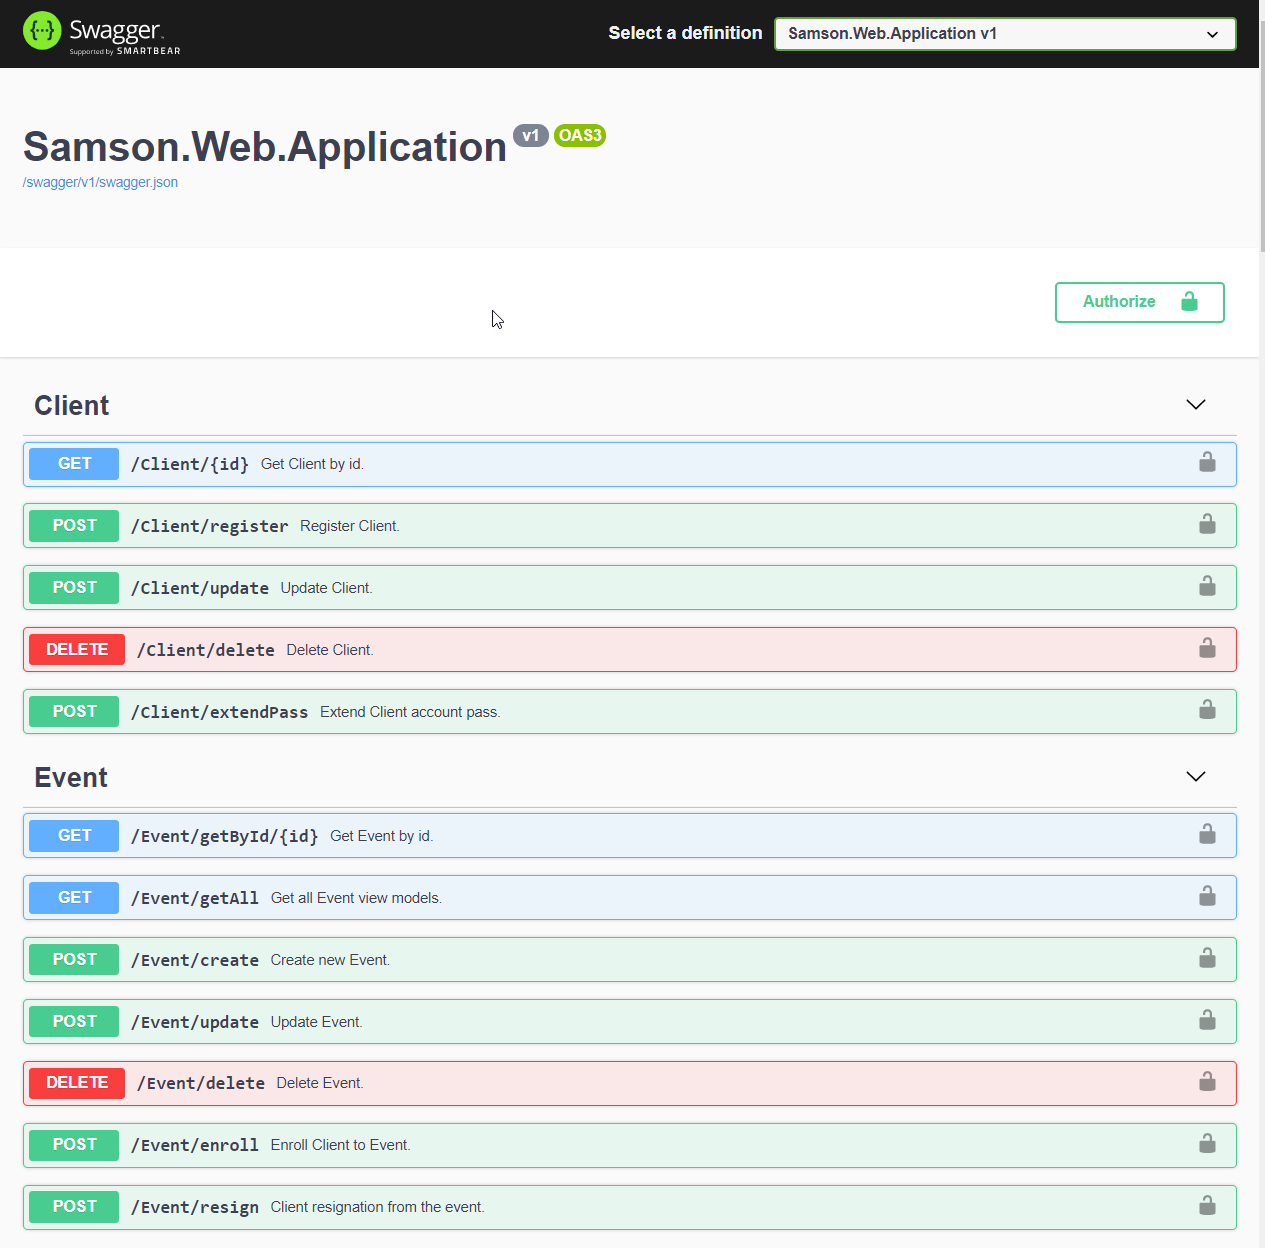
\includegraphics[width=1\linewidth]{../zrzuty_ekranu/testy/swagger}
	\caption{Interaktywna dokumentacja interfejsu \textit{REST API}}
	\label{fig:swagger}
\end{figure}
Przy pomocy wcześniej wspominanej dokumentacji przetestowano poprawność działania końcówek (ang. \ang{endpoint}) interfejsu \textit{REST API}. Natomiast w celu całościowego sprawdzenia poprawności działania systemu wykonano szereg testów manualnych przy wykorzystaniu warstwy prezentacji. System był testowany według scenariuszy, które odpowiadają funkcjonalnościom przedstawionym w podrozdziale \textbf{\nameref{UseExample}}.

\section{Organizacja testów}
Podczas pracy nad systemem równolegle tworzono kod testów jednostkowych, aby już w trakcie implementacji funkcjonalności wykrywać błędy w kodzie. Część błędów została wykryta już na etapie uruchamiania kodu testów jednostkowych. W takim przypadku poprawiono kod implementujący daną funkcjonalność w celu usunięci błędu. Inne błędy zostały wykryte w trakcie testów manualnych. W takim przypadku potrzebna była dodatkowa analiza kodu aplikacji. Po zidentyfikowaniu błędu, zostawał on usuwany, a następnie w celu uniknięcia przyszłych nieprawidłowości dopisywano test jednostkowych, którego zadaniem było dopilnowanie by taka sytuacja się nie powtórzyła.

\section{Przykłady wykrytych i usuniętych błędów}
W trakcie pracy nad systemem wykryto, dzięki testom kilka błędów wynikających z niepoprawnej implementacji. Jednym z przykładów niepoprawnego działania, było usuwanie konta użytkownika zamiast jego archiwizacja. Gdy ten sam użytkownik był zapisany na jakiś trening lub wydarzenie, a konto zostało usunięte całkowicie z bazy to w danych pojawiły się relacje do nieistniejącego konta co prowadziło do licznych błędów.

Poprzedni błąd został wykryty przez testy manualne, natomiast udało się wykryć błąd przy pomocy testu jednostkowego. W systemie istnieje moduł, który odpowiada za kontrolę liczby osób, która znajduje się na siłowni. Maksymalna liczba osób była obliczana w niepoprawny sposób z powodu wykonywania dzielenia zamiast mnożenia. Poprawiona funkcja została zaprezentowana na Kod \ref{lst:calcMaxPeople}
\begin{lstlisting}[caption={Metoda licząca jaka jest maksymalna liczba osób, która znajduje się w~jednej chwili w~obiekcie siłowni}, label={lst:calcMaxPeople}]
	public int CalcMaximumClientsCount()
	{
		if (CovidConfiguration == null)
		return -1;
		
		var availableGymObjectArea = GymObjectArea();
		/* (int) Math.Floor(availableGymObjectArea / CovidConfiguration.PersonFactorPerMeter); */
		return (int) Math.Floor(availableGymObjectArea * CovidConfiguration.PersonFactorPerMeter);
	}
\end{lstlisting}

Wykorzystanie interaktywnej dokumentacji \textit{Swagger} pozwoliło na wykrycie błędów we wczesnym etapie tworzenia aplikacji. W systemie wykorzystano bibliotekę \textit{AutoMapper}, która pozwala na mapowanie obiektów z jednej klasy na inną według zdefiniowanego schematu. Gdy taki schemat nie został zdefiniowany, a funkcja \textit{Map} została wywołana to o błędzie użytkownik dowiadywał się dopiero gdy aplikacja została już uruchomiona. W takich przypadkach interaktywna dokumentacja pozwoliła na wykrywanie błędów i ich usuwanie jeszcze przed utworzeniem interfejsu użytkownika.

\chapter{Podsumowanie i wnioski}
\label{chap:summary}
Praca nad projektem przyniosła rezultaty w postaci systemu spełniającego określone wcześniej wymagania. Udało się pokryć zakres funkcjonalny związany z~obostrzeniami pandemicznymi, co było główną przesłanką do rozpoczęcia prac nad nim. Wybór aplikacji internetowej pozwolił na utworzenie systemu dostępnego dla większości systemów operacyjnych. Poza spełnieniem wymagań funkcjonalnych, udało się również wykorzystać nowoczesne technologie, które zapewniają dłuższe wsparcie producentów.

W ramach projektu udało się stworzyć dokument, który opisuje sposób działania systemu oraz ideę, która za nim stała. W trakcie tworzenia systemu położono nacisk na architekturę, która pozwoli na skalowanie. Poza tym zwrócono również uwagę na odpowiednią dokumentacje kodu, aby rozwiązanie mogło być rozwijane w~kilkuosobowym zespole. Zaproponowana architektura pozwala również na zmianę architektury monolitycznej na mikro-usługową, co pozwoliłoby na pracę w większych zespołach.

Stworzenie systemu w oparciu o dokumentową bazę danych pozwoliło na wykorzystanie zalet technologii \textit{NoSQL}. Szczególnie pomocny był elastyczny schemat bazy. Początkową strukturę można było utworzyć na podstawie wcześniej utworzonych modeli, a następnie zoptymalizować je w celu poprawy wydajności. Aby to osiągnąć wykorzystano denormalizację danych w celu przechowywania informacji rzadko aktualizowanych. Takie podejście pozwoliło na poprawę czasu odczytu. Wadą tego rozwiązania jest wydłużony czas zapisu oraz potrzeba manualnego kontrolowania czy wszystkie powiązane dokumenty zostały zaktualizowane, dlatego technikę tą wykorzystywano tylko w przypadku gdy dane są bardzo często odczytywane, ale rzadko aktualizowane.

Mimo, że rozwiązanie posiada wiele cech produktu komercyjnego, wymaga ono dopracowania w warstwie prezentacji. Niektóre z widoków powinny zostać zaprojektowane na nowo, tak aby były bardzie intuicyjne dla użytkownika. Poza poprawieniem przejrzystości formularzy, kolejnym krokiem w rozwoju systemu powinno być dostosowanie aplikacji do zasad RWD. Jest to istotne ze względu na duży udział urządzeń mobilnych w generowaniu ruchu na stronach internetowych \cite{bib:mobileVsDesktop}.

Na rynku komercyjnym znajduje się wiele innych rozwiązań, które oferują większe możliwości pod względem funkcjonalnym. Naturalnym krokiem byłoby dodanie modułu recepcji oraz barów z odżywkami dla klientów. Poza nowymi modułami rozszerzone powinny być również te istniejące. Moduł karnetów powinien zostać rozszerzony o integracje z systemem płatności. Na rynku znajduje się wielu pośredników, którzy udostępniają API pozwalające na płatność w wygodny dla klienta sposób.

W celu komercjalizacji systemu ważne jest dodanie ról dla pozostały pracowników sieci siłowni. Konto trenera personalnego powinno mieć inne uprawnienia od konta administratora systemu. Natomiast w razie dodania modułu recepcji istotne byłoby dodanie roli recepcjonisty, który nie potrzebowałby dostępu do modułu treningów indywidualnych.
 
\bibliographystyle{plplain}
\bibliography{bibliografia}
\addcontentsline{toc}{chapter}{Bibliografia}

\begin{appendices}
 

\chapter*{Spis skrótów i symboli}
\addcontentsline{toc}{chapter}{Spis skrótów i symboli}

\begin{itemize}
	\item[API] aplikacyjny interfejs programistyczny (ang. \ang{Application programming interface})
	\item[CRUD] utwórz, odczytaj, aktualizuj, usuń - (ang. \ang{Create, Update, Read, Delete})
	\item[CQRS] (ang. \ang{Command and Query Responsibility Segregation})
	\item[DTO] obiekt transferu danych (ang. \ang{Data transfer object})
	\item[HTTP] (ang. \ang{Hypertext Transfer Protocol})
	\item[HTTPS] (ang. \ang{Hypertext Transfer Protocol Secure})
	\item[IDE] zintegrowane środowisko programistyczne (ang. \ang{Integrated development environment})
	\item[JS] (ang. \ang{JavaScript})
	\item[JSON] (ang. \ang{JavaScript Object Notation})
	\item[JWT] (ang. \ang{JSON Web Token})
	\item[MVC] model -- widok -- kontroler (ang. \ang{model--view--controller}) 
	\item[NoSQL] nierelacyjna baza danych
	\item[LINQ] (ang. \ang{Language-Integrated Query})
	\item[REST] (ang. \ang{Representational state transfer})
	\item[RWD] (ang. \ang{Responsive web design})
	\item[SDK] zestaw narzędzi dla programistów (ang. \ang{Software development kit})
	\item[SPA] jednostronicowa aplikacja internetowa (ang. \ang{Single page application})
	\item[SQL] (ang. \ang{Structured Query Language})
	\item[TS] (ang. \ang{TypeScript})
\item[WWW] światowa rozległa sieć komputerowa (ang. \ang{World Wide Web})
\end{itemize}


\chapter*{Źródła}
\addcontentsline{toc}{chapter}{Źródła}
\begin{lstlisting}[caption={Klasa \textit{MongoRepository}}, label={lst:mongoRepository}, nolol=true]
	public abstract class MongoRepository<TModel, TEntity> : IRepository<TModel> where TModel : IAggregate where TEntity : IEntity
	{
		protected readonly IMongoCollection<TEntity> Collection;
		protected readonly IMapper Mapper;
		
		public MongoRepository(IDatabaseConfiguration databaseConfiguration, IMapper mapper)
		{...}
		
		public MongoRepository(IDatabaseConfiguration databaseConfiguration, IMapper mapper, string collectionName)
		{...}
		
		public TModel Get(ObjectId id)
		{...}
		
		public List<TModel> Get()
		{...}
		
		public Task<ObjectId> Create(TModel model)
		{...}
		
		public Task<ObjectId> Update(ObjectId id, TModel updatedModel)
		{...}
		
		public Task<ObjectId> Remove(TModel modelToDelete)
		{...}
		
		public Task<ObjectId> Remove(ObjectId id) => ...
	}
\end{lstlisting}

\chapter*{Spis załączników elektronicznych}
\addcontentsline{toc}{chapter}{Spis załączników elektronicznych}

Do pracy dołączona jest następującą zawartością:
\begin{itemize}
\item praca - praca.pdf,
\item źródła - źródła.zip,
\item dokumentacja - dokumentacja.zip
\item prezentacja - prezentacja.pptx
\item film z prezentacją działania - film.zip
\end{itemize}

\listoffigures
	
\lstlistoflistings
	
\end{appendices}


\end{document}


%% Finis coronat opus.
